\documentclass[a5paper]{memoir}
% \usepackage{verse}
\usepackage{polyglossia}
\usepackage[center, sc]{titlesec}
\usepackage{s24options}
\usepackage{pdfpages}

% Set up fonts to use Hindi
\newfontfamily\devtransl[Mapping=DevRom]{Times New Roman}
\setmainlanguage{english}
\setotherlanguages{hindi}
\newfontfamily\hindifont{Noto Sans Devanagari}[Script=Devanagari] % Use any Devanagari font on your system

% set up formating for the verse package
\newcommand{\attrib}[1]{\nopagebreak{\raggedleft\footnotesize #1\par\newpage}}
\renewcommand{\poemtitlefont}{\normalfont\large\bfseries\centering}

% Create the chapter format using titlesec
\titleformat
{\chapter}
[display] %shape
{\HUGE} %format
{\Roman\filcenter Chapter \thechapter} % label
{1cm} %sep
{\centering} % before code
[\newpage] % after code

%%%%%%%%%% BOOK INFORMATION %%%%%%%%%%
\newcommand{\authorname}{\texthindi{डॉ जुगिन्दर लूथरा}}
\newcommand{\booktitle}{\texthindi{जीवन यात्रा}}
\newcommand{\subtitle}{Subtitle}
\newcommand{\publisher}{Your Publisher}
\newcommand{\editionyear}{2024}
\newcommand{\isbn}{0000}   
\title{\booktitle}
\author{\authorname}


\begin{document}
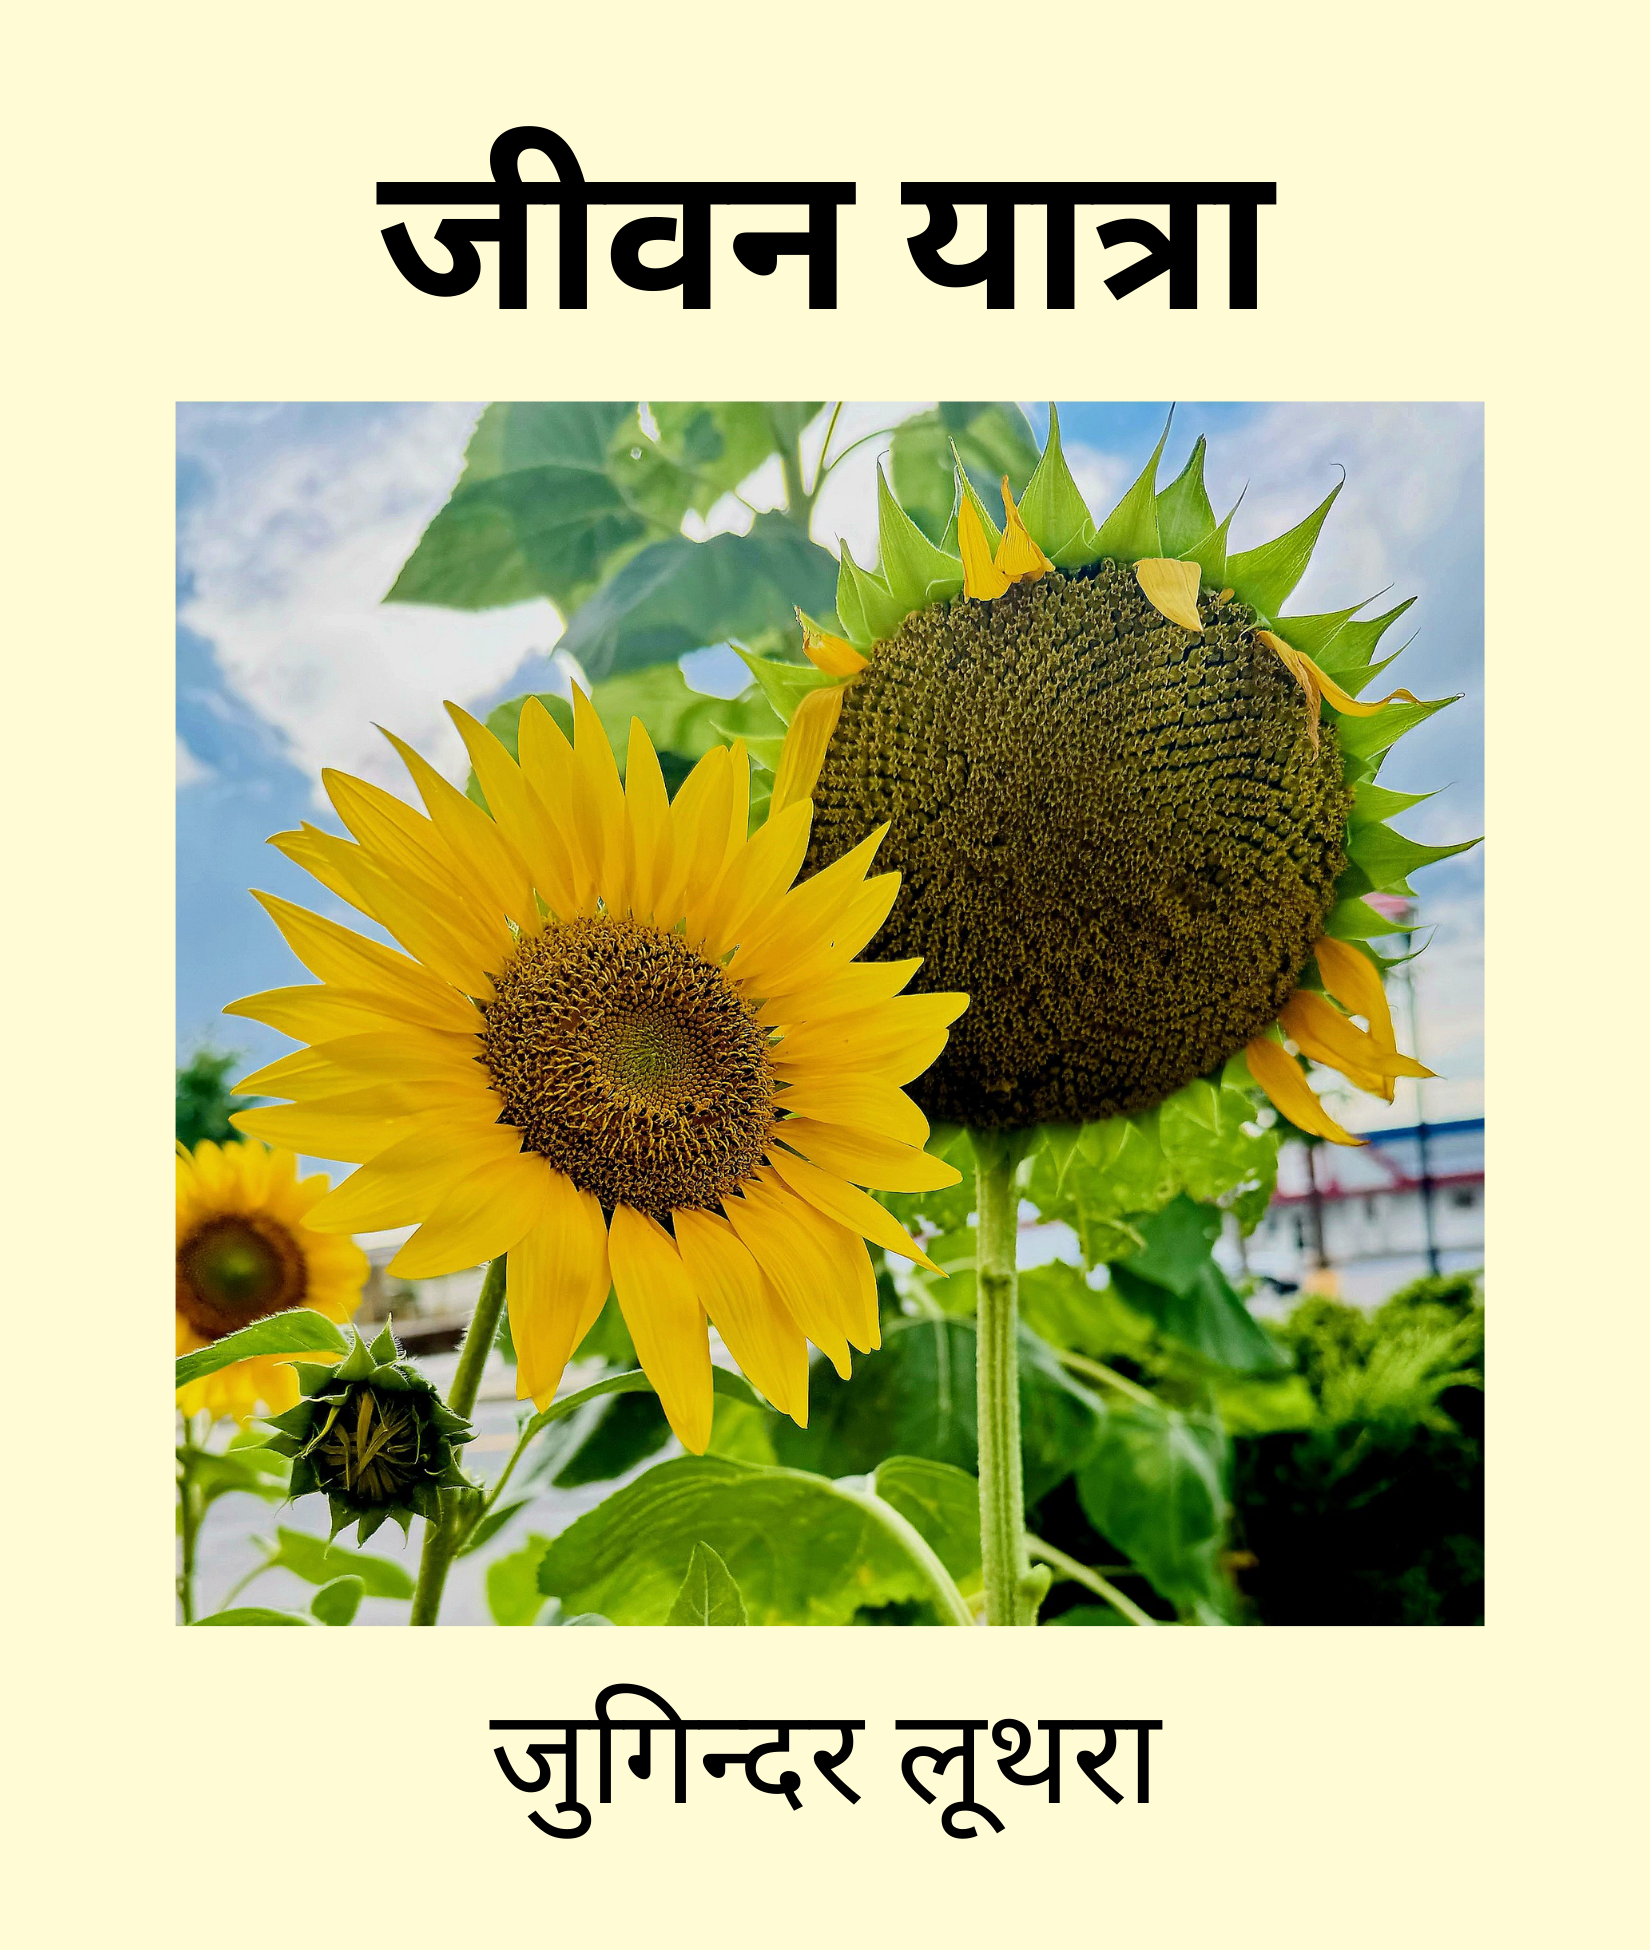
\includepdf{s24_cover.png}
\frontmatter
\pagestyle{empty}

% Half title page
{
\centering

~

\vspace{24pt}
% {\scshape\Huge \booktitle \par}
}
\cleardoublepage

% Title page
\begin{titlingpage}
	\centering
	
	~
	
	\vspace{24pt}
	{\scshape\Huge \booktitle\par}
	\vspace{6pt}
	{\scshape\large \subtitle\par}
	\vspace{\stretch{1.25}}
	{\itshape\large by\par}
	\vspace{6pt}
	{\itshape\Large \authorname\par}
	\vspace{\stretch{6}}
	{\large \publisher\par}
\end{titlingpage}
\centering
\texthindi{
कॉपीराइट पृष्ठ \\
इस पुस्तक की सभी कवितायें जुगिन्दर लूथरा  द्वारा संरक्षित है। सभी अधिकार सुरक्षित हैं। इस पुस्तक के किसी भी हिस्से को लेखक और प्रकाशक की लिखित इजाज़त के बिना डुप्लीकेट, या किसी भी रूप में या किसी भी माध्यम से उपयोग नहीं किया जा सकता है। \\
प्रकाशक: प्रकाशक का नाम \\ 
प्रथम संस्करण
}:2024\\
\centering
ISBN:\texthindi{नंबर }
\thispagestyle{empty}
\tableofcontents
\cleardoublepage
\chapter{Preface}
\texthindi{
इस किताब की यात्रा को पूरा करने में बहुत\\
लोगों ने सहायता की है। मेरी तुकबंदियों को\\
कविता का दर्जा दे कर मुझे प्रोत्साहन दिया\\
है। उन के सहयोग और प्रोत्साहन के बिना\\
इसे पूरा करना संभव नहीं था।\\
डॉ शिववरण सिंह रघुवंशी, जयदेव तनेजा, कृष्णा शर्मा, आरती पिंटो, पंकज महरोत्रा का इस किताब के पूरा होने में हाथ है। मेरी पत्नी, डौली लूथरा ने कविताओं को सुना और संवारा। नमिता रोहिनी और रश्मी ने किताब लिखने लिए प्रोत्साहित किया। प्रेम लूथरा ने कविता लिखने की योग्यता देखी \\
हमारे दोहते, अर्जन बीर सिंह ने फूलों की तस्वीर स्वयं लेने के बाद पुस्तक का आवरण बहुत प्यार और लगन के साथ बनाया। नमिता लूथरा ने कई सुझाव दिये। \\
अंत में, उन अनगिनत व्यक्तियों का धन्यवाद\\
करता हूँ जिन्होंने इस यात्रा में अपने\\
अनुभव, कहानियाँ और सुझाव मेरे साथ\\
साझा किये—आप सभी ने इस पुस्तक में\\
हो और योगदान दिया है।आप ने दिल से सराहना कर के मेरा हौसला बढ़ाया।\\
यह पुस्तक मैं अपने गुरु जी को, अपने परिवार और आप सब को समर्पित करता हूँ\\
जुगिन्दर लूथरा
}

\mainmatter
\pagestyle{fancy}
%Chapter 1
\chapter{\texthindi{क्रम}}

\poemtitle{\texthindi{आध्यात्मिक}}

\settowidth{\versewidth}{This is the average line and so is this}
\begin{verse}[\versewidth]\texthindi{
\texthindi
भगवान\\
स्रोत\\
सर्वव्यापी\\
मोक्ष\\
दो दिन का मेहमान\\
असली रूप\\
खुदी\\
नाशुक्रा\\
दो राहें\\
जीवन का मकसद
}
\end{verse}

\poemtitle{\texthindi{परिवार}}
\begin{verse}[\versewidth]\texthindi{
दो नम्बर मकान\\
पहला मिलन\\
मुहब्बत\\
नाचूँ खुशियों से\\
लगता है मैं घर आ गया हूँ\\
मैं कहाँ फँस गया हूँ\\
अपनी मिट्टी\\
हमारा बचपन\\
दिल करता है\\
व्यापारी की इज़्ज़त\\
माँ\\
उर्मिल की कहानी\\
प्रेम लूथरा श्रद्धांजली\\
एफ़ जी टी मर गई\\
जीवन\\
अब नहीं तो कब\\
एक फूल की कहानी\\
पुनर्जन्म\\
सुखी जीवन\\
सरसराहट\\
निंदा\\
कल\\
वक्त\\
वक्त या पैसा\\
खुशी अन्दर है\\
बाँट के चीज़\\
शब्द शक्ति\\
खोखली हंसी\\
ये वक्त जाने कहाँ चला गया
}
\end{verse}

\poemtitle{\texthindi{ज़िन्दगी}}
\begin{verse}[\versewidth]\texthindi{
बात\\
नये पंछी\\
रौशनी की इज़्ज़त\\
इन्सान की इज़्ज़त\\
चाँद\\
दोस्त\\
नकली दोस्त\\
अतीत के भूत\\
सवेरा\\
आग में सुलगना\\
कच्चे घड़े\\
बच्चों की मुस्कुराहट\\
नया जीवन\\
छे फ़ुट का फ़ासला\\
साथी\\
घर लुटवाना\\
औरत\\
काश हम मिले न होते\\
काश हम बिछड़े न होते\\
जीवन पथ\\
दर्दे दिल\\
गुस्सा\\
एक हाथ की ताली\\
मकड़ी जाल\\
राजनेता\\
पुनर्मिलन\\
नज़रिया\\
किस्मत के धनी\\
रामायण सारांश में\\
महाभारत सारांश में\\
सुनामी\\
इक रब के कई नाम\\
घड़ी
}
\end{verse}

\poemtitle{\texthindi{हास्य}}
\begin{verse}[\versewidth]\texthindi{
बाँके लाल का ढाबा\\
पोकर\\
बीवी\\
पति\\
पति पत्नी की नोक झोंक\\
पैसे के दो रूप\\
शराबी\\
आधुनिक दीवाली\\
जॉनी का सर दर्द\\
जीवन\\
कोविड के दिन, जाऊँ तो जाऊँ\\
महँगे प्याज़\\
फ़ोन\\
स्टॉक्स\\
अमेरिका के कुछ काँटे\\
सत्तर्वाँ जन्म दिन\\
बुढ़ापा बीमारी मौत\\
बड़ती उम्र\\
मेरी उम्र\\
खोई जवानी\\
दोस्तों की नई तस्वीरें\\
बुढ़ापे के रंग\\
आल्ज़ाइमर्ज़\\
जीवन का खेल\\
बहुत देर\\
मोम के पुतले\\
जन्म मरण\\
मौत\\
यादों के खँडरात\\
दुआ\\
जीवन और मौत\\
जीवन का अन्त\\
समय की धूल
}
\end{verse}

\chapter{\texthindi{आध्यात्मिक}}

\poemtitle{\texthindi{भगवान}}
\begin{verse}[\versewidth]\texthindi{
बिन बुलाए मेहमान घर में नहीं आते\\
मैं कब से तैयार तुम ही नहीं बुलाते\\
दिल से बुलाओ छुपे भगवान चले आते\\
दिल से बुलाओ छुपे भगवान चले आते\\
\\
तेरे न्योते के इंतज़ार में आँखें बिछाये\\
बार बार सोचूँ कब नींद से जग जाये\\
गहरी नींद में तुम ने कितने जन्म गंवाये\\
ना धन से ना हीरे मोती से मुझे सजाये\\
बैठा सच्चे प्यार लगन की आस लगाये\\
\\
तेरी शोहरत ताकत पैसा मुझ से मिलता\\
मेरे हुक्म बिना पत्ता भी ना हिलता\\
ना कर लोभ गुमान क्रोध ईर्षा शिकायत\\
जितना कर्मों ने कमाया उतना ही मिलता\\
\\
प्यार से खिला रूखी सूखी खा लूँ\\
पैरों में आ जाये उठा गले लगा लूँ\\
है अंश मेरा क्यों खुद से जुदा बना लूँ\\
अपनी मैं छोड़ दे, तुझे अपने में मिला लूँ\\
अपनी मैं छोड़ दे, तुझे अपने में मिला लूँ
}
\end{verse}

\poemtitle{\texthindi{स्रोत}}
\begin{verse}[\versewidth]\texthindi{
माँग जहाँ से सब कुछ आये\\
माटी से क्यों आस लगाये\\
बीज अक्षर तेरे बीच रमा है\\
जो सारा संसार चलाये\\
माँग जहां से...\\
\\
कोई जन धन से महान कहाये\\
कोई तन से बलवान कहाये\\
सुंदर काया शव कहलाये\\
जिस तन से श्री राम सिधाये\\
राम ही धन है, राम ही शक्ति 2\\
राम ही बेड़ा पार लगाये\\
माँग जहाँ से सब कुछ आये\\
माटी से क्यों आस लगाये\\
माँग जहां से...\\
\\
जीवन एक हवा का झोंका\\
आज उठा है कल ना रहे गा\\
ये मेरा है वो मेरा है\\
वो तो रहे गा तू ना रहेगा\\
राम सदा थे राम सदा हैं\\
जुग जुग चाहे बीत ही जायें\\
माँग जहाँ से सब कुछ आये\\
माटी से क्यों आस लगाये\\
बीज अक्षर तेरे बीच रमा है\\
जो सारा संसार चलाये\\
माँग जहां से…
}
\end{verse}

\poemtitle{ \texthindi{ सर्वव्यापी } }
\begin{verse}[\versewidth]\texthindi{
देखूँ जिधर मैं तुझ को पाऊँ\\
जब जब तेरा ध्यान लगाऊँ\\
देख तेरी लीला महिमा मैं गाऊँ\\
जोड़ के हाथों को सीस झुकाऊँ\\
\\
देखूँ जिधर मैं तुझ को पाऊँ\\
जब जब तेरा ध्यान लगाऊँ\\
\\
कोई तोहे राम कहे कोई हरि पुकारे\\
वाहे गुरु अल्लाह यीशु नाम तिहारे\\
जिस नाम से भी तुझ को पुकारूँ\\
पल में तेरा दर्शन पाऊँ\\
देखूं जिधर…\\
\\
दरस तेरा उस को मिल जाता\\
जिस पे कृपा हो जाये तेरी दाता\\
चरणों में तुम रख लो मुझ को\\
दर दुनिया मैं छोड़ के आऊँ\\
देखूँ जिधर...\\
\\
पाप की गठरी ढो कर आया\\
लाया वही जो मैं ने कमाया\\
दे दो सहारा ओ मेरे मालिक\\
मैली चादर धो कर जाऊँ\\
\\
देखूं जिधर मैं तुझ को पाऊँ\\
जब जब तेरा ध्यान लगाऊँ\\
देख तेरी लीला को\\
महिमा मैं गाऊँ\\
जोड़ के हाथों को सीस झुकाऊँ \\
जोड़ के हाथों को सीस झुकाऊँ
}
\end{verse}

\poemtitle{ \texthindi{ मोक्ष } }

\begin{verse}[\versewidth]\texthindi{ 
पलक झपकते जीवन बीता\\
पंछी को उड़ जाना है\\
कौन है अपना कौन पराया\\
दो दिन का ये ठिकाना है\\
पलक झपकते…\\
\\
बचपन बीता आई जवानी\\
फूल ही फूल थे रुत मस्तानी\\
काल खड़ा देखे राहें तेरी\\
छोटी सी है ये ज़िंदगानी\\
राम से मन का मेल मिला ले x2\\
तन तो यहीं रह जाना है\\
पलक झपकते…\\
\\
जिन से मोह ममता कर बैठे\\
वो ना कभी तुम्हारे थे\\
जन्म जन्म का जिन से नाता\\
उन को ही क्यों बिसारे थे\\
भगवन तुझ से दूर नहीं है x2\\
एक ही बार बुलाना है\\
पलक झपकते…\\
\\
झूठी काया झूठी माया\\
मृग तृष्णा में क्यों भरमाया\\
राम स्वरूप सुनहरा पंछी\\
तन की आँख से देख ना पाया\\
बाहर माटी में तू ढूँढे x2\\
मन के बीच खज़ाना है\\
पलक झपकते…\\
\\
काम क्रोध मद मोह और माया\\
हथकड़ियाँ बन जायें गे\\
मात पिता सुत बीवी भाई बहना\\
साथ ना तेरे जायें गे\\
सच्चे कर्म और नाम राम का x2\\
साथ ही तेरे जाना है\\
पलक झपकते…\\
\\
गुरु और गुर की महिमा जानो\\
राम का रूप हैं तुम पहचानो\\
गुरु कृपा देखो दीप जला कर\\
राह दिखाये ओ अनजानो\\
तन से पूजो मन से ध्याओ x2\\
आत्म लीन हो जाना है\\
पलक झपकते…\\
\\
गुरु ने राम से मेल कराया\\
राम का निश दिन ध्यान करो\\
राम नाम की नाव में चढ़ कर\\
भव सागर को पार करो\\
जन्म मरण का खेल मिटा कर x2\\
मोक्ष तुझे अब पाना है\\
पलक झपकते जीवन बीता\\
पंछी को उड़ जाना है\\
कौन है अपना कौन पराया\\
दो दिन का ये ठिकाना है\\
पलक झपकते…
}
\end{verse}

\poemtitle{ \texthindi{दो दिन का मेहमान
}} \begin{verse}[\versewidth]\texthindi{ 
दो दिन का मेहमान रे तू\\
खुद को अब पहचान रे तू x2\\
कल तू आया कल है जाना\\
काहे करे अभिमान रे तू\\
दो दिन का मेहमान रे तू\\
\\
जिस को तू ने घर है समझा\\
ये तो एक सराये है\\
सदा नहीं कोई रहता इस में\\
इक आये इक जाये है\\
इक आये इक जाये है\\
राम शरण में तुझ को जाना\\
वहीं लगा ले रे ध्यान तू\\
दो दिन का मेहमान रे तू\\
\\
कौड़ी कौड़ी माया जोड़ी\\
लाख कमाए फिर भी थोड़ी\\
इस पैसे के लालच ने\\
सब रिश्तों की कड़ी है तोड़ी\\
सब रिश्तों की कड़ी है तोड़ी\\
हाथ तो खाली जाना है\\
झूठी बनाए क्यों शान रे तू\\
दो दिन का मेहमान रे तू\\
\\
जिस माटी ने तुझे बनाया\\
उस में ही मिल जाना है\\
जब तक तू है इस दुनिया में\\
कर्म भला कर जाना है\\
कर्म भला कर जाना है\\
दुखियों का दुःख बाँट ले बन्दे\\
जन्म का कर कल्याण रे तू\\
दो दिन का मेहमान रे तू\\
\\
दो दिन का मेहमान रे तू\\
खुद को अब पहचान रे तू\\
कल तू आया, कल है जाना\\
काहे करे अभिमान रे तू\\
दो दिन का मेहमान रे तू
}
\end{verse}

\poemtitle{ \texthindi{असली रूप
}}\begin{verse}[\versewidth]\texthindi{ 
मन मंदिर में घोर अंधेरा\\
जोत जले हो जाये सवेरा\\
मूँद के आँखें ध्यान लगा लो\\
तन तेरा है राम का डेरा\\
मन मंदिर…\\
\\
मंदिर मस्जिद गुरुद्वारा मन\\
दर दर भटके क्यों प्राणी जन\\
श्वास की धारा में बह कर देखो x2\\
कण कण में राम जी का बसेरा\\
मन मंदिर में…\\
\\
सुषमणा खोलो कुंडलिनी जागे\\
तन मन लागें कच्चे धागे x2\\
प्राणायाम से योग मिला लो x2\\
उस से असली जो रूप है तेरा\\
\\
मन मंदिर में घोर अंधेरा\\
जोत जले हो जाये सवेरा\\
मूँद के आँखें ध्यान लगा लो\\
तन तेरा है राम का डेरा\\
तन तेरा है राम का डेरा
}
\end{verse}

\poemtitle{ \texthindi{खुदी
}}\begin{verse}[\versewidth]\texthindi{
खुदी को मार दो खुद मरने से पहले\\
फिर देखो जीने का मज़ा क्या है\\
अंदर झाँक के देखो रब का रूप\\
इधर उधर भटकने में रखा क्या है\\
\\
यही रब मुझ में जो छुपा तुझ में\\
अलग नाम देने का फ़ायदा क्या है\\
दीन धर्म मज़हब इंसानों की हैं देन\\
असल को खिताबों से लेना क्या है\\
\\
जिधर भी देखो उस की ही सृष्टि\\
समझो उस बीच रमा क्या है\\
उस की सोच से तेरी बहुत छोटी\\
होता वही जो उस की रज़ा है\\
\\
जीवन डोर उसे थमा दे जो सारा संसार\\
चलाए\\
वही बनाए वही चलाए फिर मिटा के नया\\
बनाए\\
इंसान को खुदी की ज़रूरत क्या है\\
खुदी को मार दो खुद मरने से पहले\\
फिर देखो जीने का मज़ा क्या है\\
फिर देखो जीने का मज़ा क्या है
}
\end{verse}

\poemtitle{ \texthindi{नशुकरा
}}\begin{verse}[\versewidth]\texthindi{
गिनती खत्म हो जाती है\\
जब तेरी मेहरबानियाँ गिनता हूँ \\
आँख झुक जाती है शर्म से\\
जब और भी मिन्नतें करता हूँ \\
\\
भूला भटका नाशुकरा लोभी\\
फिर से भिखारी बन जाता हूँ \\
भूल खिलौने तोहफ़े सेहत\\
खुशी के नये साधन अपनाता हूँ \\
\\
जो मिला मुझे मेरी मेहनत थी\\
जो ना दिया गिला तुझ से\\
अपनों से ऊँचों को देख जलूँ\\
भूला सभी जो मिला तुझ से\\
\\
जब देखूँ अंधे को, कुछ पल\\
आँखों पे गरुर आ जाता\\
देखूँ शव, इक हल्का एहसास\\
खुद ज़िंदा होने का आ जाता\\
\\
सोचूँ दुःख बीमारियाँ मौत\\
रब ने बनाये दूजों के लिए\\
मैं तो सदा रहूँ गा ज़िंदा\\
हस्पताल शमशान दूजों के लिए\\
\\
फिर इक दिन कैन्सर या\\
दिल का दौरा पड़ जाता\\
इक बुलबुला हूँ सागर में\\
साफ़ दिखाई पड़ जाता\\
\\
तब सोचूँ कितना दिया तू ने\\
जिसे मैं ने नज़र अन्दाज़ किया\\
भाई बहन साथी घर छोड़े\\
रब सेहत को भुला बस\\
पैसे शान का नशा पिया\\
\\
आधी बन्द आँखें बेहोशी में\\
अंत ख्याल मुझे आता\\
पर किस्मत वाला तेरी मेहर से\\
जल्द ज्ञान पा जाता\\
क्या ?\\
गिनती खत्म हो जाती है\\
जब तेरी मेहरबानियाँ गिनता\\
आँख झुक जाती है शर्म से\\
जब और भी मिन्नतें करता
}
\end{verse}

\poemtitle{\texthindi{दो राहें
}}\begin{verse}[\versewidth]\texthindi{
दो राहें तेरे मन को मिलीं थी\\
एक को क्यों तू ने छोड़ दिया\\
एक को क्यों तू ने छोड़ दिया\\
\\
भूल गया तुझे जिस ने बनाया\\
भटका जहाँ उस की है माया\\
माया मृग छाया है भोले x2\\
उस के पीछे क्यों दौड़ लिया\\
एक को क्यों तू ने छोड़ दिया...\\
\\
सूरज जिस से रौशनी पाये\\
जो सारा संसार चलाये\\
उस दीपक से उस शक्ति से\\
मुख को क्यों तू ने मोड़ लिया\\
एक को क्यों तू ने छोड़ दिया ...\\
\\
दो राहें तेरे मन को मिलीं थी\\
एक को क्यों तू ने छोड़ दिया\\
एक को क्यों तू ने छोड़ दिया
}
\end{verse}

\poemtitle{\texthindi{ जीवन का मकसद 
}}\begin{verse}[\versewidth]\texthindi{
तर्ज़ — तू गंगा की मौज\\
है सदियों से ये सवाल चलता ही आया x2\\
काहे कुदरत ने इंसान जहाँ क्यों बनाया\\
\\
गीता में अर्जुन ने कृष्ण से पूछा\\
कृष्ण से पूछा\\
कल युग में शिक्षक ने गुरुओं से पूछा\\
गुरुओं से पूछा\\
रब ने बनाया तुझे प्रेम खज़ाना\\
प्रेम खज़ाना\\
गम अपना भूल तुझे जग को हँसाना\\
हर कोई अपना है ना कोई पराया\\
काहे कुदरत ने…\\
\\
किस्मत तू लिखे हाथों से अपनी\\
हाथों से अपनी\\
मिलता वो ही फल जो बोये तेरी करनी\\
बोये तेरी करनी\\
मन छोड़ बुद्धि से काम जो ले तू\\
काम जो ले तू\\
रब तेरे संग है अकेला नहीं तू\\
सफ़र ज़िंदगी में वो तेरा ही साया\\
काहे कुदरत ने इंसान जहां क्यों बनाया\\
है सदियों से ये सवाल चलता ही आया x2\\
काहे कुदरत ने इंसान जहाँ क्यों बनाया
}
\end{verse}

% Page 55 of 518
\chapter{ \texthindi{परिवार} }

\poemtitle{ \texthindi{दो नंबर मकान } }
\begin{verse}[\versewidth]\texthindi{
आओ सब मिल गायें गाथा\\
दो नंबर मकान की\\
सन पचास में बोली लगा कर\\
लगा दी बाज़ी जान की\\
मात पिता की जै बोलो\\
मात पिता की जै\\
मात पिता की जै बोलो\\
मात पिता की जै\\
लाला जी को दस एकड़\\
ज़मीं मिली ईनाम में\\
कुंदन बेटा बने गा डॉक्टर\\
करम ज़मीं के काम में\\
कुदरत के रंग किस्मत पलटी\\
करम मिले श्री राम में\\
छोड़ डॉक्टरी के सपने\\
कुंदन खेती के काम में\\
ना शिकवा ना गिला था कोई\\
चेहरे पर मुस्कान थी\\
आओ सब मिल गायें गाथा\\
दो नंबर मकान की\\
मात पिता की जै बोलो\\
मात पिता की जै\\
\\
सरगोधे से चली ये जोड़ी\\
पहुँची खानेवाले में\\
पिता बाईस के माता जी थी\\
अभी सोलहवें साल में\\
पिता जी ने मारा छक्का\\
सब से पहली बॉल में\\
क्रिकेट टीम के कैप्टेन सूरज\\
पहुँचे पहले साल में\\
रेलवेज़ का अफ़सर हो गा\\
शान हिंदुस्तान की\\
आओ सब मिल गायें गाथा\\
दो नंबर मकान की\\
मात पिता की जै बोलो\\
मात पिता की जै\\

सुदेश मोहिन्दर लाँघ ना पाये\\
बचपन की दीवार को\\
प्रेम कांता कंचन विरिंदर\\
शोभा दें संसार को\\
कृशन गिंदी शोकी ने कर दिया\\
पूरा लंबी कतार को\\
मात पिता ने सींची क्यारी\\
दे कर अपने प्यार को\\
जीवन धारा बहती जाये\\
खबर ना पाकिस्तान की\\
आओ सब मिल गायें गाथा\\
दो नंबर मकान की\\
मात पिता की जै बोलो\\
मात पिता की जै\\
\\
खानेवाले में धूप की गर्मी\\
नफ़रत की थी आग जली\\
दूर दर्शी हिंदू जनता\\
सदियों के घर से भाग चली\\
पिता जी नारंग ठक्कर भाई\\
छुपा प्यारी हर दिल की कली\\
दूर सबाथु ठंडी छाँव में\\
परिवार की नाव चली\\
मई सैंतालिस जान बचा कर\\
ढूँढी जगह विश्राम की\\
आओ सब मिल गायें गाथा\\
दो नंबर मकान की\\
मात पिता की जै बोलो\\
मात पिता की जै\\
\\
जहाँ भी देखो लाशें थीं\\
हर तरफ़ खून की होली थी\\
हा हा कार था आग और धुआँ\\
मार पीट की टोली थी\\
सदियों से जो भाई बहन थे\\
अब नफ़रत की बोली थी\\
पानीपत घर छीन लिया\\
जो जगह थी मुसलमान की\\
\\
आओ सब मिल गायें गाथा\\
दो नंबर मकान की\\
मात पिता की जै बोलो\\
मात पिता की जै\\
\\
जिधर भी देखो टैंट लगे थे\\
हर कोई घर की आस में\\
रेल लाइन के पार था प्यारा\\
इक घर खुले आकाश में\\
दो नंबर पर नज़र पड़ी\\
पिता जी की तलाश में\\
बीवी बच्चे यहीं पलें\\
हरियाली और प्रकाश में\\
मां ने ना की पैसा ना पल्ले\\
बोली दी मकान की\\
आओ सब मिल गायें गाथा\\
दो नंबर मकान की\\
मात पिता की जै बोलो\\
मात पिता की जै\\
आओ सब मिल गायें गाथा\\
दो नंबर मकान की\\
मात पिता की जै बोलो\\
मात पिता की जै\\
\\
(यह कविता मैं माता जी और पिता जी को\\
अर्पित करता हूँ। हम भारत के उस हिस्से में थे\\
जो अब पाकिस्तान में है।\\
तर्ज़—आओ बच्चो तुम्हें दिखायें झांकी हिंदुस्तान)
}
\end{verse}

\poemtitle{ \texthindi{पहला मिलन}}
\begin{verse}[\versewidth]\texthindi{
याद है जब हम पहली बार मिले थे\\
थामा पहली बार नर्म काँपता हाथ\\
उँगलियों ने चेहरे से बाल हटाए\\
आँख झुकी “आप बोलती बहुत\\
अच्छा हैं।”\\
\\
बिजली जिस्म में फैली होंठ थर्राए\\
छोटी छोटी बातों पे रूठ जाया करते\\
रात की नींद दिन का चैन गवाया करते\\
कई सुंदर सपने दिन में बनाया करते\\
हवा में रंग बिरंगे महल सजाया करते\\
हाथों पे तरह तरह तेरा नाम लिख\\
अपने नाम से जोड़ा करते\\
ना रिश्तों का बोझ ना पीछे का गम\\
खुश आपस में गिले ना करते\\
\\
उत्सुकता थी दिल में घबराहट काफ़ी थी\\
याद है जब हम पहली बार मिले थे\\
याद है जब हम पहली बार मिले थे
}
\end{verse}

\poemtitle{\texthindi{मुहब्बत}}
\begin{verse}[\versewidth]\texthindi{
मुहब्बत मानो शब्दों में लायी नहीं जाती\\
हकीकत जो ज़बान से समझाई नहीं जाती\\
फूल की खुशबू हवाओं में रम जाती\\
हल्की मुस्कान दिल को है भाती\\
दिलों की बात चेहरे पे लाई नहीं जाती\\
मुहब्बत…\\
\\
झुकी आँखें होंठ काँपते दिल का राज़ बताते\\
गाल गुलाबी माथे पसीना खुद से वो शर्माते\\
अपनो से क्या परदा बात छुपाई नहीं जाती\\
मुहब्बत…\\
\\
ना पैसे की इसे चाहत ना ढूँढे कोई बड़ा नाम\\
बंगला ना शोहरत इसे बस दिल से है काम\\
ये रब की मेहर, दौलत से कमायी नहीं जाती\\
मुहब्बत…\\
\\
दिल की बात दिल जाने कहने से क्या लेना\\
नज़र नीची ने कह डाला होंठों को सी लेना\\
रूह बात करे रूह से मुँह से बताई नहीं जाती \\
मुहब्बत मानो शब्दों में लायी नहीं जाती\\
हकीकत ऐसी ज़ुबान से समझाई नहीं जाती
}
\end{verse}


\poemtitle{\texthindi{नाचूँ खुशियों से}}
\begin{verse}[\versewidth]\texthindi{
नाचूँ मैं खुशियों से रात दिन\\
मुझे मेरा प्यार मिला\\
यार मिला दिल दार मिला\\
नाचूँ मैं खुशियों से रात दिन\\
\\
जब से मैं ने होश सम्भाला\\
तुम्हें ही चाहा तुम्हें ही माँगा\\
राह में ठोकर जब मोहे लागी\\
बाँह पकड़ कर तू ने सम्भाला\\
जो भी मैं ने माँगा रब से\\
उस से ज़्यादा मिला\\
नाचूँ मैं …\\
\\
दिल में उमंगें लब पे तराने\\
सपनों ने ली है अंगड़ाई\\
फूल खिले हैं इस बगिया में\\
देखूँ जिधर बहार है छाई\\
कलियों के अब दिन आये हैं\\
करूँ क्या रुत से गिला\\
नाचूँ मैं खुशियाँ से रात दिन\\
मुझे मेरा प्यार मिला\\
यार मिला दिल दार मिला\\
नाचूँ मैं खुशियों से रात दिन
}
\end{verse}

% page 79 of working version.docx
\poemtitle{\texthindi{लगता है मैं घर आ गया हूँ
}}\begin{verse}[\versewidth]\texthindi{
ये कविता मैं भारत को, अपनी मातृ भूमि को\\
अर्पण करता हूँ। जो भारत छोड़ आये हैं,\\
आओ घर चलते हैं।\\
\\
खुदगर्ज़ी से खुशहाली पाने देश था छोड़ा\\
मात पिता भाई बहनों से नाता था तोड़ा\\
उन सुनहरी यादों को ताज़ा कर लेता हूँ\\
कदम जहाज़ से बाहर जब रखता हूँ\\
लगता है मैं घर आ गया हूँ\\
\\
इमीग्रेशन क्लर्क में देखूं बाप की परछाई\\
सर ओढ़े आँचल में माँ लौट के वापस आई\\
सड़क पे खेलते बच्चों बीच खुद को ढूंढूँ\\
शोर गुल में बचपन के खोये यारों को ढूंढूँ\\
बाहर निकलते ऐसे नज़ारे देखता हूँ\\
लगता है मैं घर आ गया हूँ\\
\\
पड़ोसी को मिलने का न्योता ना चाहिए\\
हमारे घर आये हो, चाय तो पी के जाइये\\
दो रोटी और बना लें गे, खाना यहीं खाइये\\
ऐसी प्यार भरी बातें सुनता हूँ\\
लगता है मैं घर आ गया हूँ\\
\\
जहां बड़ों कि इज़्ज़त अभी भी होती\\
अंत समय अकेले रहने नहीं देती\\
जहां बच्चे बढ़े बूढ़ों को कंधा देते\\
सर झुका पैरों को छू दुआ हैं लेते\\
ऐसी पुरानी रीतें देखता हूँ\\
लगता है मैं घर आ गया हूँ\\
\\
पड़ोसी जब चाहे दरवाज़ा खटका सकता है\\
मिलने को खास वक्त ज़रूरी ना समझता है\\
फ़ासला उन के अपने घर का मिट जाता है\\
ऐसे बड़े परिवार को साथ साथ देखता हूँ\\
लगता है मैं घर आ गया हूँ\\
\\
बड़े आदमी ताऊ और चाचा औरत\\
 मासी कहलाती है\\
हर बच्चा बच्ची अपनी ही बेटा \\
बेटी कहलाती है\\
जहां रिश्तों का मिट जाता है फ़र्क \\
अपने पराये में\\
 घुल मिल प्यार से सब का रहना देखता हूँ\\
लगता है मैं घर आ गया हूँ\\
\\
रेल गाड़ी में तेज़ “चाय गरम” की पुकार\\
पोटली से निकलें परांठे आम का अचार\\
मुँह में पानी आ जाता है, माँग लूँ?\\
दिल में आये विचार\\
“आप भी दो बुर्की ले लो”\\
अनजान हमसफ़र कहता है\\
दो रोटी सफ़र में खाता हूँ\\
लगता है मैं घर आ गया हूँ\\
\\
लाउड स्पीकर सुबह सुबह रब के गीत सुनाये\\
राम, वाहे गुरु, अल्लाह की ऊँची महिमा गाये\\
कोयल की मधुर आवाज़ सोये सपनों से जगाये\\
सुरीली आवाज़ों में माँ बाप से जफ्फी लेता हूँ\\
लगता है मैं घर आ गया हूँ\\
\\
दीवाली में जगमग देश हुआ होली में बना सतरंग\\
लोहड़ी में सुंदर मुंद्रिये राखी भाई बहिन के\\
संग\\
नवरात्रे, कंजकें, दसहरा हर मौके पे होता\\
सत्संग\\
जब ऐसे अपने अनेक त्यौहार देखता हूँ\\
लगता है मैं घर आ गया हूँ\\
\\
वो उड़ती पतंगें, पैंचे लड़ाना\\
दीवारों छतों पर दीयों का सजाना\\
गुल्ली डंडा, पिट्ठू, कंचों की आवाज़\\
कौओं की कैं कैं का शोर मचाना\\
नल से खींच ठंडे पानी में\\
ठिठुर के नहाना\\
राह चलते ऐसे भूले नज़ारे देखता हूँ\\
लगता है मैं घर आ गाया हूँ\\
\\
हवा महके जगाये भूली बिसरी यादें\\
धूल में अपनी मिट्टी की खुशबू\\
माँ बाप की फरियादें\\
खस खस सी सुगंध पहली बारिश की\\
ठंडी हवा\\
पानी से पेड़ घर की दीवारें धुलते देखता हूँ\\
लगता है मैं घर आ गया हूँ\\
\\
माँ बाप दादा नानी की ज़िंदगी दोहरायी जाती\\
भाई बहनों की दौड़ धूप कहानी सुनायी जाती\\
ज़िंदगी की ऊँच नीच, हालातें बताई जाती\\
बचपन से आज की खुली किताब देखता हूँ\\
लगता है मैं घर आ गया हूँ\\
\\
और फिर \\
बिछड़ते वक्त कैदी आंसुओं का छुपाना\\
अनकहे फिर ना मिलने के ख्यालों का आना\\
वो हाथों का पकड़ना फिर न छुड़ाना\\
लम्बी प्यार भारी जुदाई, कंधे सहलाना\\
टपकते सुर्ख आंसुओं में सोचता हूँ\\
लगता है मैं घर छोड़े जा रहा हूँ\\
\\
करता हूँ खुद से वादा, जल्द दोहराऊँ गा\\
लगता है मैं घर आ गया हूँ\\
\\
सुनसान हैं गलियाँ ना बन्दों की आवाज़\\
अजनबी चेहरे भाषा अलग यहाँ के साज़\\
पड़ोसी पड़ोसी को ना जाने\\
अपनों को भी न पहचाने\\
सालों से साथ है इन का\\
फिर भी लगते हैं अनजाने\\
\\
बिन वजह रोज़ गोलियों का चलना\\
मासूम बच्चों बड़ों का बन्दूकों से मरना\\
ऐसी जगह से हर साल वापिस लौटता हूँ\\
तो लगता है मैं घर आ गया हूँ\\
मातृ भूमि में आ गया हूँ\\
पितृ भूमि में समा गया हूँ\\
मैं अपने ही घर वापस आ गया हूँ\\
लगता है मैं घर आ गया हूँ\\
लगता है मैं घर आ गया हूँ
}
\end{verse}

\poemtitle{\texthindi{मैं कहाँ फँस गया हूँ 
}}\begin{verse}[\versewidth]\texthindi{
जब में ने कविता-“लगता है मैं घर आ गया\\
हूँ” लिखी तो मेरे भाई, प्रेम, ने कहा “भाई, \\
पढ़ के मज़ा आ गया और बहुत अच्छा लगा। \\
तुम ने ऐसी चीज़ें भी देखी, झेली हों गी जो\\
तुम्हें परेशान करती हैं। उस को मध्य नज़र\\
रखते हुए कुछ लिखो”\\
\\
लगभग बीस साल पहले ये कविता लिखी\\
थी। कई चीज़ें अभी भी लागू हैं। अब तो\\
भारत कई तरह से इतना बदल गया है की ये\\
शायद अब नहीं लिख पाता। ये परिवर्तन देख\\
कर बहुत खुशी और गर्व होता है।\\
\\
डेंगू टाइफाइड और मलेरिया\\
मखी मछरों का है राज\\
दूध में ज़्यादा नल में कम पानी\\
कूड़ा गलियों का सरताज\\
खुली नालियां, हवा में बदबू\\
पुरानी गलियाँ वैसी ही आज\\
बचपन की ऐसी निशानियाँ\\
देखता हूँ\\
सोचता हूँ मैं कहाँ फँस गया हूँ\\
\\
सड़कों पर वही भीड़ भड़का\\
ट्रकों का जहां राज है पक्का\\
सब को शिक्षा देता पिछवाड़ा\\
बुरी नज़र वाले तेरा मुँह काला\\
माँ का आशीर्वाद जय जय माता\\
डिप्पर एट नाईट ओ के टाटा\\
ट्रकों से लटकते गन्ने खींचें बच्चे\\
लगता है मैं फिर बचपन में आ गया हूँ\\
\\
मेट्रो मैं चड़ूँ जेबों को बचाऊं\\
खाने को देखूं, खाऊं ना खाऊं\\
पेट खराब हो गा ज़रूर\\
डॉक्टरों के चक्कर में न फँस जाऊं\\
हस्पताल बने पैसे की मशीने\\
बैंक बैलेंस खाली ना कर जाऊं\\
रोज़ बचाव के तरीके ढूंढता हूँ\\
सोचता हूँ मैं कहाँ फँस गया हूँ\\
\\
बदन कांपता है यहाँ की सर्दी से\\
फेफड़े बंद हुए धूएँ और गर्दी से\\
चोरी डकैती बलात्कारी\\
दिल दहल गया आवारागर्दी से\\
अरे यारों, शिकायत करें किस से\\
डर लगता यहाँ खाकी वर्दी से\\
ऎसे दुःख भरे हालात देखता हूँ\\
सोचता हूँ मैं कहाँ फँस गया हूँ\\
\\
कुर्सी खातिर आया राम गया राम हैं अभी\\
नाम बदले उन के पर काली हरकतें हैं अभी\\
देश में छाया अन्धकार रौशन इन का घर\\
कानून आम आदमी पर ना इन्हें कोई डर\\
नये चेहरों पे राजनीति पुरानी देखता हूँ\\
सोचता हूँ मैं कहाँ फँस गया हूँ\\
\\
हर काम के लिए जानकारी या रिश्वत लाओ\\
यहाँ का दस्तूर खुद खाओ दूजों को खिलाओ \\
मंत्री से ले चपरासी का रास्ता पैसे का\\
पर नारे ज़ोर से लगाते दुराचार हटाओ!\\
ये सालों पुरानी तरकीबें देखता हूँ\\
सोचता हूँ मैं कहाँ फँस गया हूँ\\
\\
चलते हुए देखता हूँ सामने तो\\
थूक कुत्तों की देन पे फिसलता\\
देखूं जो नीचे कार से जा टकरता\\
घर से बाहर जब मैं निकलता\\
बचाऊं खुद को सामने या नीचे से\\
सोचता हूँ कहाँ फँस गया हूँ\\
\\
लिखा है 'गधा पेशाब कर रहा है' \\
मगर आदमी खड़ा है\\
बिन वजह भौंकता कुत्तों का झुण्ड \\
निकल पड़ा है\\
सड़क पे उलटी तरफ कार स्कूटर चल पड़ा है\\
लाल बत्ती में ड्राईवर बेधड़क निकल पड़ा है\\
ऎसे अजब नज़ारे देखता हूँ\\
सोचता हूँ कहाँ फँस गया हूँ\\
\\
पक्की टिकट थी ट्रेन और प्लेन की\\
उसे भी उन्हों ने रद्द कर डाला\\
बहाने बनायें पर सच तो ये था\\
मिनिस्टर या वी आई पी आने वाला\\
सफ़र बन जाता है सफ्फ़र जहां\\
डाँटना दुतकारना झेलता हूँ\\
सोचता हूँ कहाँ फँस गया हूँ\\
\\
इंडिया का सफ़र बहुत लम्बा लगता\\
टी एस ए, थ्रोमबोसिस से डर लगता\\
जेट लैग सात दिन इधर भी उधर भी\\
दो हफ़्ते का सफ़र चार का बनता\\
ऎसे कष्ट भरे दिन देखता हूँ\\
सोचता है कहाँ फँस गया हूँ\\
\\
अब गिनता दिन घर वापस जाने के\\
बिन सोचे हरी सलाद खाने के\\
दोहते दोहतियों को गोद बिठाने के\\
उत्तर हो या दक्षिण घर अपना मन भाये\\
परिंदे छोड़ पुराना घोंसला नया बसाये\\
हर जगह फूल और कांटे अपने अपने\\
राह जो चुनी वहीं अपने सपने सजाये\\
ऎसे ख्यालों में डूबा जहाज़ में बैठता हूँ\\
इक घर छोड़ मैं दूजे घर जा रहा हूँ\\
\\
वो भी मेरा ये भी मेरा जहाँ भी जाता हूँ\\
लगता है मैं घर आ गया हूँ
}
\end{verse}

\poemtitle{\texthindi{अपनी मिट्टी }}
\begin{verse}[\versewidth]\texthindi{
गुज़रे साल पचास छोड़े अपना देश\\
मिट्टी उस की अभी भी अपनी लगती है\\
मिट्टी उस की अभी भी अपनी लगती है\\
\\
पहले लोग कहते बेटा भाई अब अंकल\\
जिस नाम से मुझे पुकारें\\
ज़ुबान उन की मीठी लगती है\\
\\
हवा नज़ारे रस्में लोग लगें अपने\\
जैसे कभी ना बिछड़े थे\\
कोयल की धुन मीठी\\
कुत्ते की भौं भौं भी अच्छी लगती है\\
\\
छुपी यादें खोल आँखें लें अंगड़ाई\\
पेड़ की छाया गर्म लू से बचाती\\
पैसा एक ना पल्ले न थे हम गरीब\\
प्यार भरी भरपूर ज़िंदगी\\
हर कमी को पूरा करती है\\
गुज़रे साल पचास छोड़े अपना देश\\
मिट्टी उस की अभी भी अपनी लगती है\\
मिट्टी उस की अभी भी अपनी लगती है
}
\end{verse}

\poemtitle{\texthindi{हमारा बचपन
}}\begin{verse}[\versewidth]\texthindi{
हम आठ, साइकल एक\\
भरपूर थी हमारी खुशी\\
इक निक्कर कमीज़\\
चप्पल का जोड़ा खज़ाना था\\
हर जश्न मनाते धूम धाम से\\
प्यार भर देता था खुशी\\
\\
माँ बाप मुसकाते चुपके पीते ज़हर\\
शहद हमें पिलाते थे\\
खुद रह कर भूखा\\
मक्खन लदे पराँठे हमें खिलाते थे\\
इक बादशाही ज़िंदगी से\\
इक दिन में बने खानाबदोश\\
ना जाने कै से हंस के\\
राज गद्दी पे हमें बिठाते थे\\
\\
पेड़ों पे आम अमरूद नहीं\\
मीठा अमृत मिलता था\\
तंदूर से आग नहीं, नर्म सेक\\
दिल को सुकून मिलता था\\
\\
पैसा एक ना पल्ले\\
घर शीश महल दिखता था\\
खुशियों के फव्वारे गूंजते\\
बेफ़िक्र सुख चैन मिलता था\\
\\
नाम पानीपत पर अक्सर नल में पानी नहीं था\\
दो हाथ पम्प थे कसरत कोई गिला नहीं था\\
कभी आयी कभी गई \\
बिजली खेले आँख मिचौली\\
हाथ के पंखे, मोम बत्ती\\
कमियों का पता नहीं था\\
\\
कभी गुल्ली डंडा पिठ्ठु\\
कभी क्रिकेट की थी बारी\\
कँचे लुक्कन छुप्पी झूला\\
गुलेल से पथरी मारी\\
\\
पढ़ाई क्या चीज़ है\\
उस बारे कम सोचा था\\
अभी है बचपन खेलो कूदो\\
पढ़ने लिखने को उम्र है सारी\\
\\
हवा में पतंगें फल फूल ज़मीं पे\\
भर देते रंगीन नज़ारा\\
ना परवाह दूजों पास है क्या\\
घड़ा रहता भरा हमारा\\
आँगन दिन में खेल मैदान\\
मच्छरदानी में तारों नीचे\\
सोने का कमरा हमारा\\
\\
बचपन के अनमोल दौर की\\
तस्वीरें जब मन में खोलूँ\\
न गम न ज़्यादा सपने\\
बस वर्तमान ही काफ़ी था\\
\\
स्वामी जी शकुन्तला दर्शी\\
माँ का आशीर्वाद बरसता है\\
ऐसा सुंदर सुहाना बचपन\\
किस्मत वालों को मिलता है\\
\\
जैसे हवा में खुशबू, तालाब में\\
रंगीन कमल खिलता है\\
ऐसा सुंदर बचपन\\
किस्मत वालों को मिलता है\\
ऐसा सुंदर बचपन\\
किस्मत वालों को मिलता है
}
\end{verse}

\poemtitle{\texthindi{दिल करता है}}
\begin{verse}[\versewidth]\texthindi{
दिल करता है उड़ कर आऊँ\\
चंद घड़ियाँ तेरे साथ बिताऊँ\\
प्यार की गंगा निस दिन बहती\\
आ के अपनी प्यास बुझाऊँ\\
दिल करता है…\\
\\
जो बिछड़े हैं काश वो होते\\
प्यार के फूलों की माला पिरोते\\
मात पिता भाई बहनों को\\
दिल से कैसे भुलाऊँ मैं\\
दिल करता है…\\
\\
बचपन की यादें दोहरायें\\
भूले बिसरे गीत सुनायें\\
उन यादों को दिल से लगा कर\\
सालों साल बिताऊँ मैं\\
दिल करता है…\\
\\
खुशी की चादर में गम छुपाये\\
हर कोई अपना बोझ उठाये\\
एक अकेला थक जाये गा\\
आ के हाथ बटाऊँ मैं\\
दिल करता है…\\
\\
जन्म मरण तक साथ है अपना\\
चार दिनों का है ये सपना\\
सपनों को रंगों से भर दूँ\\
खुशियों के फूल चढ़ाऊँ मैं\\
दिल करता है…\\
\\
दिल करता है उड़ कर आऊँ\\
चंद घड़ियाँ तेरे साथ बिताऊँ\\
प्यार की गंगा निस दिन बहती\\
आ के अपनी प्यास बुझाऊँ\\
दिल करता है
}
\end{verse}

\poemtitle{\texthindi{व्यापारी की इज़्ज़त
}}\begin{verse}[\versewidth]\texthindi{
सामान बेच रही हूँ मैं इज़्ज़त तो नहीं\\
झुक रही हूँ ना समझना गैरत ही नहीं\\
\\
गरीब शायद पैसे से शराफ़त से नहीं\\
करती मेहनत पैसे खातिर चोरी नहीं\\
\\
घर बच्चों की परवरिश करना है धर्म\\
लोगों की गाली सुनने का शौक नहीं\\
प्यार से बात करो पैसे से ना तोलो मुझे\\
मुस्कान देने से दौलत घटती तो नहीं\\
\\
आवाज़ ऊँची कर इंसान बड़ा नहीं बनता\\
हल्का सर्द झोंका देता सुकून, तूफ़ान नहीं\\
\\
ना देखो मुझे शक की निगाह से\\
थमाओ हाथ में, फेंको नहीं पैसे\\
काम करती हूँ भिखारी तो नहीं\\
\\
सामान बेच रही हूँ मैं इज़्ज़त तो नहीं\\
झुक रही हूँ ना समझना गैरत ही नहीं\\
\\
माँ\\
सन्देश आया तेरे घर से\\
माँ की आँखें तेरी राह को तरसे\\
पिछले सावन वो बोली थी\\
अर्थी निकले गी अब इस घर से\\
सन्देश आया…\\
\\
तन से अपना दूध पिलाया\\
भूखे रह कर तुझे खिलाया\\
अपने मन की चाह मिटा कर\\
तेरा सपना सार कराया\\
शिकवा ज़बान पर कभी ना लाई\\
प्यार सदा आँखों से बरसे\\
सन्देश आया...\\
\\
मन ही मन वो घबराती थी\\
जल्द बुढ़ापा आये गा\\
बेटा डॉक्टर बन जाने पर\\
वक्त पे काम वो आये गा\\
उस के सपने टूट गये जब\\
पाँव निकाला तू ने घर से\\
सन्देश…\\
\\
माया खातिर जाल बिछाया\\
जाल में अपना आप गंवाया\\
मात पिता को छोड़ा तू ने\\
यादों पर भी पड़ गया साया\\
यादों के वो महल हैं खाली\\
महल निवासी निकले घर से\\
\\
सन्देश आया तेरे घर से\\
माँ की आँखें तेरी राह को तरसे\\
पिछले सावन वो बोली थी\\
अर्थी निकले गी अब इस घर से\\
सन्देश आया…\\
\\
उर्मिल की कहानी\\
\\
सुनो छोटी सी लड़की की लम्बी कहानी\\
सारी दुनिया से न्यारी प्यारी सी नानी\\
सुनो छोटी सी लड़की की कहानी\\
\\
राम पिता थे और सरला थी माता\\
छोटी सी गुड़िया के नंदी हैं भापा\\
नाना नानी से सुख प्यार बहुत पाया\\
आँख जब खुली न देखा बाप का साया\\
दिन सात बाद मिला उन्हें गंगा का पानी\\
सुनो…\\
\\
गुड़ियों से खेला और वायलिन बजाया\\
छोड़ पाकिस्तान लुधियाना घर बनाया\\
चीनी घर में थोड़ी पर बाँट इस ने खाई\\
यौवन में आई तो सूरज से की सगाई\\
नौ साल बाद पिया पानीपत का पानी\\
सुनो…\\
\\
चाँद सा चेहरा और आँखें हैं तारों सी\\
लौ से चमके डार्लिंग सूरज प्यारे की\\
पहले पहुंची निशी फिर आरती घर आई\\
साथ साथ करती थी बी एड की पढ़ाई\\
सिर पे ना ताज था सूरज बुलाये रानी\\
सुनो…\\
\\
मोम जैसा दिल चट्टान जैसा सर है\\
बाल धो के निकली तेल से वो तर है\\
आम चूसे निम्बू का आचार मन भाये\\
तीस नंबर घर में मेहमान सदा आये\\
इस शोर गुल में इनकी बीती जवानी\\
सुनो…\\
\\
छोड़ जोधपुर को दिल्ली घर बनाया\\
रेलवे कालोनी फिर आनंद विहार बसाया\\
ब्रिज इन की सौतन बैडमिंटन से प्यार था\\
बच्चों के ऊंचे नंबर दिलाने का विचार था\\
मॉडर्न स्कूल में वो बन गई मास्टरानी\\
सुनो…\\
\\
फिर क्या हुआ आरती?\\
\\
पार्किन्सन सिर सढ़िया का दिल इन पे आया\\
सुरमिल की ताकत ने दूर तक भगाया\\
जिस्म थक जाये अन्दर से ताकतवर है\\
परिवार का प्यार सेवा दवा का असर है\\
अंत हुए कष्ट बीमारी करे खत्म ज़िन्दगानी\\
सुनो छोटी सी लड़की की लम्बी कहानी\\
सारी दुनिया से न्यारी प्यारी सी नानी\\
सुनो छोटी सी लड़की की कहानी\\
(उर्मिल की श्रद्धांजली आरती की सहायता से
लिखी गयी है)
}
\end{verse}

\poemtitle{\texthindi{प्रेम लूथरा श्रद्धांजलि
}}\begin{verse}[\versewidth]\texthindi{
बूढ़ी हड्डियां कमज़ोर हुईं\\
जोड़ भी अब जुड़ने लगे\\
थक गया दिल धड़कते धड़कते\\
सांस भी अब रुकने लगे\\
\\
दौड़ धूप से झुलसा कोमल बदन\\
जिस्म कमज़ोर उठते नहीं कदम\\
जीने का कोई मकसद ना देखूँ\\
अंदर बाहर मैं थक गया हूँ\\
\\
कैंसर ने घर मुझ में बनाया\\
चोर के माफ़िक वो घुस आया\\
लाख दवा और दुआएँ करवाईं\\
फिर भी उस से जीत ना पाया\\
\\
एक म्यान में दो तलवारें रह ना पाएं\\
दुश्मन इक दूजे को सह ना पाएं\\
मैदाने जंग में हम ने की बहुत लड़ाई\\
उस कातिल से हम जीत ना पाए\\
\\
अब दिल करता है मैं सो जाऊँ\\
ऐसी नींद कि उठ नहीं पाऊँ\\
अपने मरने का डर नहीं लगता\\
बोझा अपनों पे ना बन जाऊँ\\
\\
अपने जाने का गम नहीं मुझे\\
डरता हूँ सोच तेरा चुप के रोना\\
बुरा शगुन तुझे कहेगी दुनिया\\
अकेले ज़िंदगी के बोझ का ढोना\\
\\
थोड़ा और जीने को मन करता\\
अपनों से दिल कभी नहीं भरता\\
कुछ और पल तेरा दामन ना छूटे\\
घुट गले लगाने को दिल करता\\
\\
काश उन संग वक्त बिताया होता\\
कल मिल लें गे जल्दी क्या है ?\\
काश ऎसा ख्याल आया ना होता\\
ज़िंदगी को और गले लगाया होता\\
\\
काश जिन्हें दुःख दिया उन्हें सताया ना होता\\
ना चिंता ना मुसीबत में घबराया होता\\
अपनों को इज़हारे मोहब्बत कराया होता\\
दुनिया को प्यार से और सहलाया होता\\
\\
प्यार लेन देन थी मेरी पहचान\\
दो चार दिन के संगी साथी\\
जैसे आये और गये मेहमान\\
अब फूलों की सेज बना हूँ\\
कल तस्वीर दीवारों की पहचान\\
\\
दिन होते लम्बे पर ज़िंदगी छोटी\\
इक इक पल गिनते बीता\\
उम्र दो पल में है खोती\\
\\
कल की है बात बचपन था जवानी थी\\
आज मैं ने दुनिया से रवानी की\\
\\
कुछ मीठी यादें कुछ शिकवे गिले\\
चंद दिन मेरी बातें हों गी\\
फिर इक कागज़ पे या किसी के दिल में\\
मेरे नाम की यादें हों गी\\
\\
ऐसे ख्यालों में डूबा खोया रहता\\
पूछने पर ज़बान से कह नहीं पाता\\
मेरे ख्याल मेरे संग ही जाने दो\\
जो पराये हैं वो ना समझें मेरी बात\\
जो समझें उन्हें आँखों से कह जाता\\
\\
कुछ तो अच्छा किया हो गा\\
जब प्यार हर तरफ़ देखता हूँ\\
जो दिया था दूजों को\\
अब वापिस लौटते देखता हूँ\\
कुछ आते करने आखरी नमस्ते\\
कुछ को अपने संग मरते देखता हूँ\\
\\
आंसुओं से आटा गूंधना\\
फिर रोटी का जल जाना\\
एक के लिए बनाना\\
फिर चुप बैठ अकेले खाना\\
\\
आँखें नम हो जाती हैं\\
तेरी अकेली ज़िंदगी सोचता हूँ\\
इस सोच से दरवाज़ा मौत का\\
बंद होने से रोकता हूँ\\
\\
पर करूं क्या आज तक\\
कोई जीत ना पाया काल से\\
पचपन साल मिलीं थी खुशियां\\
मुसकाना उसी ख्याल से\\
\\
मेरे हिस्से का खाना मेरा प्यार भी दुगने लुटाना\\
कल हमसफ़र, अब तुम में मैं हूँ\\
गुज़रे तू जिस भी हाल से\\
\\
जिस्म ना सही, रूह सदा तेरे साथ है\\
रहना सुखी हर हाल में तेरे सर पे मेरा हाथ है\\
जितने दिन मिले तुम्हें हँसते हुए बिताना तुम\\
यही दुआ मेरी राम से यही मेरी फ़रियाद है\\
\\
अपनी इनिंग अब पूरी कर ली मैं ने\\
जितनी लिखी उतनी रन बना लीं मैं ने\\
खुशियां बांटने से स्कोर की गिनती होती\\
फिर तो कई सेंचरी लगा दी मैं ने\\
\\
कोई तो क्लीन बाउल्ड या कौट आउट हुआ\\
\\
शुक्र है माँ बाप राम और राम शरणम् का\\
शशि अशित ज्योती दिशा तनुज सब का\\
मेरे संगी थे साथी थे इस खूबसूरत मेल में\\
सब को आउट होना है ज़िंदगी के खेल में\\
\\
अलविदा मैं सब को करता हूँ प्रेम से\\
ये मेरा आखरी खत है तुम्हारे प्रेम से\\
\\
फ़ॉण्डली प्रेम
}
\end{verse}

\poemtitle{\texthindi{एफ़ जी टी मर गई
}}\begin{verse}[\versewidth]\texthindi{
कोई खबर ना ज़िक्र है उस का\\
लगता है वो शायद मर गयी है\\
चर्चे सुनते चार दिन उस के\\
ज़िंदाबाद ज़ोर शोर के नारे\\
लूथरा खानदान इतिहास पन्नों में\\
शायद उस का ज़िक्र तो हो गा\\
एक या दूजी पीढ़ी पढ़ेगी मुस्कुराते\\
मीठी यादें खोने का फ़िक्र तो हो गा\\
अब मुलाकात होती चमकते फ़ोन पे\\
झुकी आँखें उँगलियों से\\
कौन करे तकलीफ़\\
घर काम छोड़ सफ़र करने से\\
अब वट्स ऐप रहे ज़िंदाबाद\\
हिंग लगे ना फटकड़ी\\
मुलाकात हो जाए\\
अब तो शब्द भी सिम्बल बने \\
करनी पड़ती कम बात \\
\\
भूले सुख जफ्फी हाथ सहलाने में\\
मुस्करा आँख से आँख मिलाने में\\
भूल गए मिल खेलना हँसना हँसाना\\
खुशियाँ बाँटना कंधे सहलाना\\
सुख दुख में आँ सुओं का बहाना\\
 \\
वक्त रुकता नहीं ज़माना बदल जाता \\
कुछ अच्छा बचा ज़्यादा खो जाता\\
अपने अपने में सब मग्न\\
परिवार का टीला धूल हो जाता\\
\\
डूब गई एफ़ जी टी वक्त के अंधेरे में\\
भूल गए गीत दिल करता है उड़ कर आऊँ\\
झूले पे चंद घड़ियाँ तेरे साथ बिताऊँ\\
दो नम्बर गाथा बोसा राम की मिठाई लाऊँ\\
\\
हम बेखुदी में तुम को पुकारे का गाना\\
दिन रात खेलना मिल जुल खाना\\
आम का पेड़ क्रिकेट ताश खिलाना\\
बिन वजह हँसी के फव्वारे लुटाना\\
\\
देखूँ उन यादों की खान में\\
सुनहरी मंच के कई खिलाड़ी\\
अलविदा कह रुला कर चले गए\\
कुछ जीवन की दौड़ धूप सह रहे\\
\\
जिन्हें ये तोहफ़ा मिला था मंच का\\
चार पीढ़ी कायम हैं मिलो मिलाओ\\
उन को इस अमृत का रस चखवाओ\\
\\
वक्त ने तब्दील किया जीवन हमारा\\
मंज़ूर है स्वीकार करना धर्म हमारा\\
\\
मौत किसी की हो खासकर अपनों की\\
इक आँसू तो आ जाता है\\
जब एफ़ जी टी का ख्याल आता है\\
चलचित्र का नज़ारा सामने आता है\\
पलकों से टपकता इक आँसू तो आ जाता है\\
पलकों से टपकता इक आँसू तो आ जाता है
}
\end{verse}

% page 160

\chapter{\texthindi{जीवन}}

\poemtitle{\texthindi{अब नहीं तो कब}}
\begin{verse}[\versewidth]\texthindi{
जीवन की रफ़्तार एक ही सब के लिए\\
ना चले ये तेज़ ना रुके किसी के लिए\\
छोटा हो या बड़ा राजा या रंक इंसान\\
पहुँचें एक मंज़िल जो कहलाये शमशान\\
\\
खुले हाथ से रेत जीवन से दिन निकलें\\
उम्र है छोटी लाखों सपने हैं दिल में\\
रंग से भर साकार सभी को कर लो\\
कल का सूरज आये या ना आये\\
सपना अधूरा रातों का रह ना जाये\\
जो करना है आज अभी ही कर लो\\
अब नहीं तो कब ?\\
\\
शोहरत पैसे के लालच ने बीवी बच्चे भुलाए\\
हर पल दुनियाँ में भटका नाम काम कमाए\\
खड़ा बुढ़ापा अगले चौराहे पे आस लगाए\\
बच्चे जल्द घर छोड़ अपनी राहों पे पड़ जायें\\
उन से खेलो हँसो हसाओ और दिल से सोचो\\
अब नहीं तो कब ?\\
\\
इस से पहले बीमारियाँ घर में बस जायें\\
जोड़ जुड़ें साँसें रुकें मुँह से निकले हाय\\
फूलों को दो पानी उन्हें सूखने से पहले\\
लोहे को बचा लो ज़ंग लगने से पहले\\
गुज़रा वक्त ना वापस आया कभी\\
जिस्म को संवार लो ढलने से पहले\\
अब नहीं तो कब ?\\
\\
जितनी उमंगें हैं दिल में अब पूरी कर लो\\
खुला आसमान देता तोहफ़े झोली भर लो\\
किस्मत से कुछ वक्त बचा है\\
ना दुःख दे जो करना अभी ही कर लो\\
सभी दोस्त भाइयों का यही है कहना\\
अरे भाई रुको, सुनो, जागो, गौर करो\\
अब नहीं तो कब ?\\
अब नहीं तो कब ?
}
\end{verse}

\poemtitle{\texthindi{एक फूल की कहानी}}
\begin{verse}[\versewidth]\texthindi{
उस की ज़ुबानी\\
\\
खुली हवा में मस्ती से मैं \\
इठलाता लहराता था\\
महक उभरती शोख लबों से \\
गीत मधुर मैं गाता था\\
\\
साथ थे मेरे संगी साथी \\
रंग बिरंगे और निराले\\
भँवरे तितली पीते रस उन का \\
जो छलकते किस्मत वाले\\
\\
ले के चुम्बन एक फूल का\\
 दूजे पर वो जाते थे\\
सात सुरों से मुझे रिझाने \\
\\
दूजे से सुंदर लगने के \\
नए नए साधन अपनाते\\
देख छवि पानी में अपनी \\
खुशी से इतराते शर्माते\\
\\
बहुत सुंदरता अच्छी भी है और बुरी भी\\
रंगों भरी जवानी अच्छी भी और बुरी भी\\
\\
चाहत भरा चुम्बन प्यार से \\
सहलाना अच्छा लगता था\\
अफ़सोस सुंदर चेहरा फूलों के \\
व्यापारी को अच्छा लगता था\\
\\
भरी जवानी रंगों से लदे \\
फूलों की तलाश में था\\
मुझ पर नज़र पड़ी पर \\
मुझे अभी एहसास ना था\\
\\
उस की काली नज़र ने \\
मुझ में शोहरत पैसा देखा\\
गुलदस्ते में खूब सजे गा \\
ये रंगीं सुंदर चेहरा\\
\\
मन ही मन उस कातिल ने \\
बुरी नज़र से सोचा था\\
बेखबर अनजान था मैं \\
कातिल में आशिक देखा था\\
\\
ज़ुल्मी ने चमकती कैंची निकाली झोले से\\
पकड़ गर्दन अलग किया मुझे मेरी माँ से\\
\\
एक ही झटके से दर्द दिया \\
लाखों सोये सपने तोड़े\\
दो पल खुशी की खातिर \\
मुझे और मेरे साथी जोड़े\\
\\
बेदर्दी ने बाँध रस्सी से \\
हम सब को कैदी बनाया\\
पानी भरे शीश महल में \\
बेचारों को खूब रुलाया\\
\\
शादी की खुशी मनाने \\
मेज़ों पर सब को सजाया\\
जिस की खातिर हम ने जान गंवाई \\
खून बहाया\\
वो मस्ती में माशूका से लिपटा झूमा लहराया\\
इक बार भी उस ने मुझे ना देखा\\
इक बार भी उस ने मुझे ना देखा \\
ना कुर्बानी मेरी\\
\\
शाम ढली फिर रात हुई धीमे से बात हुई मेरी\\
"बहुत सुंदर हैं ना ये फूल, बहुत महंगे हों गे"\\
मन रोया सुन ज़िंदगी के सपने पैसे में तुलते\\
\\
मेरा रोना किसी ने देखा ना दुःख समझ पाया\\
खाना पीना खत्म शुक्रिया कोई कह ना पाया\\
\\
किस्मत वाले गए किसी संग घर सजाए\\
मेरे जैसे कुचले बेचारे कचरे में समाए\\
क्या सोचा था कितने सपने दिल में थे बनाए\\
\\
अपनी ज़िंदगी रंगीन कई महीनों खिलें गे\\
इक संसार नया हो गा बीज बच्चे मिलें गे\\
\\
कोई किस्मत से लड़ नहीं पाता\\
लिखा कोई मिटा नहीं पाता\\
अब दम तोड़ रहा हूँ कूड़े के बर्तन में\\
\\
पानी में बहते मिले मेरे आँसू\\
पर दिल से दुआ देता हूँ\\
खुश रहें जिन कि खातिर\\
मेरा कत्ल हुआ खून बहा\\
लम्बी उम्र हो उन की\\
बेवक्त ना उन को कोई काटे\\
\\
आँखें बन्द किए बेहोशी में\\
बस यही दुआ देता हूँ\\
लम्बी उम्र हो उन की\\
बेवक्त ना उन को कोई काटे\\
बेवक्त ना उन को कोई काटे
}
\end{verse}

\poemtitle{\texthindi{पुनर्जन्म}}
\begin{verse}[\versewidth]\texthindi{
ये रिश्ते भी इक मौसम हैं\\
हर पल हर मास बदलते\\
साथ साथ दिन रात गुज़ारे\\
अब अपनी राह पे चलते हैं\\
\\
कल कलियाँ अब फूल खिले\\
कड़ी धूप ने इन्हें कुम्हलाया\\
ना हुई बरदाश्त कड़क गर्मी\\
घबरा के पतझड़ आया\\
\\
बिखर गये हरे लाल और पीले\\
उतरे मस्त जवानी के रंग\\
हुए बेरंग फिर भी सिमट कर\\
चिपके रहे वो मां के संग\\
\\
आया सर्द हवा का झोंका\\
रिश्ते सब कमज़ोर हुए\\
कोई पहले तो कोई पीछे\\
सब के सब झँझोर हुए\\
\\
सजा खूब बदन गुलशन का\\
हल्के रंगीन पत्तों से\\
रोयें बहुत ऊपर से शाखें\\
ले के आंसू शबनम से\\
\\
सुबह की पहली किरण देख\\
भेजें असीसें टिप टिप रे\\
“बहुत ही अच्छा लगता था\\
जब साथ सभी तुम थे मेरे\\
\\
रब से माँगूँ तेरी खुशियाँ\\
रहना तुम सदा आबाद\\
बदलना जीवन का दस्तूर\\
रखना हमेशा ये तुम याद\\
\\
ये सुंदर चमचमाता बदन\\
इक दिन ज़रूर ढल जाये गा\\
आहिस्ता आहिस्ता खामोशी से\\
तेरा रंग बदलता जाये गा\\
\\
आये गा इक दिन बाग का माली\\
जब तुम सूख जाओ गे\\
बनाये गा इक ढेर तुम्हारा\\
मेरे सामने जल जाओ गे\\
\\
जिन्हें छुपाया था आँचल में\\
अब वो खाक बन जायें गे\\
बदलियाँ बन आंसू मेरे\\
चिता तुम्हारी सहलायें गे\\
\\
ना घबराना ना रोना बच्चो\\
जड़ें तुम्हारी राह देखें गी\\
मिला के पानी बारिश का\\
तुम्हें सीने में छुपा लें गी\\
\\
बाद कड़क सर्दी के ज़रूर\\
हम फिर से मिलें गे\\
नये सावन में नये रूप में\\
हम सब हंस के खिलें गे\\
\\
सदियों से ये खेल कुदरत का\\
चलता जाये गा\\
जो आया था चला गया\\
फिर चोला बदल के आये गा\\
\\
ना फूलों में ज़्यादा खुश होना\\
ना पतझड़ में रोना तुम\\
दिल से कभी भुला ना देना\\
मेरा ही इक अंग हो तुम\\
कभी पास तो दूर कभी\\
पर हरदम मेरे संग हो तुम\\
कभी पास तो दूर कभी\\
मेरा ही इक अंग हो तुम\\
मेरा ही इक अंग हो तुम
}
\end{verse}

\poemtitle{\texthindi{सुखी जीवन}}
\begin{verse}[\versewidth]\texthindi{
बीते कल के गम दफ़ना कर\\
जोड़ो मीठे पलों की यादें\\
जीवन नए रंग दिखलाता\\
ना देखो कल के टूटे धागे\\
\\
कोई रहता अतीत में डूबा\\
कोई सीखता उस की भूलों से\\
कदम वही जो बढ़ते आगे\\
खुले आँख सिर्फ़ देखे आगे\\
\\
डूबता सूरज लाए अँधेरा\\
काट खाए जीवन का इक दिन\\
सुबह की किरण लाए नया दिन\\
गहरे सपनों से जब हम जागे\\
रब ने अपनी गिनती कर के\\
बाँटे कुछ दिन हम सभी को\\
उन में हँसी भरो या रोना\\
खुशी अब की या कड़वी यादें\\
\\
किसी बच्चे के आँसु पोंछो\\
किसी बूढ़े को दे दो सहारा\\
मज़ा देना लेने से बेहतर\\
दूजों की खुशी से अपने गम भागे\\
\\
पालती पोस्ती माँ बच्चों को\\
 अपने सारे दुःख दर्द भुला के\\
कड़वा सच है उन से छुपाती\\
उन का बचपन स्वर्ग बना दे\\
\\
इच्छा लालसा का अंत नहीं\\
इक मारो दूजी जग जाती\\
इन से दूर ही रहना सुखमय\\
समझें ज्ञान ज्योत जब जागे\\
इन से दूर ही रहना सुखमय\\
समझें ज्ञान ज्योत जब जागे
}
\end{verse}

\poemtitle{\texthindi{सरसराहट}}
\begin{verse}[\versewidth]\texthindi{
पत्ते हिले पेड़ों में सरसराहट\\
हिरण ने नज़र अन्दाज़ किया\\
छुपा शेर झपटा पल में\\
रात का खाना हज़म किया\\
\\
मदिरा पी के कार चलाई\\
दोस्तों ने बहुत मना किया\\
जवानी में किस ने देखी मौत\\
रोते बाप ने हाथों आग लगाई\\
\\
टेनिस खेलते एक दोस्त ने\\
अंदर बॉल को बाहर कहा\\
ना सोचा, उस संग धंधा किया\\
अब ना पैसा ना दोस्त रहा\\
\\
मैं सिगरेट नहीं पीता मना किया\\
मेरी लिये एक ले लो बोला दोस्त\\
सरसराहट ना समझा ना पहचाना\\
चल बसा घर वालों को रुला दिया\\
\\
रब ने सही आवाज़ सब में छुपायी\\
काम क्रोध मद लोभ की धूल छाई\\
आवाज़ बचपन की जवानी ने खाई\\
अब वो लगे सरसराहट की परछाई\\
\\
गर जीवन को सही राह पे लाना\\
साँसों में हो लीन रब को पाना\\
रामायण गीता से धूल हटा कर\\
सरसराहट की आवाज़ फिर जगाना\\
सरसराहट की आवाज़ फिर जगाना
}
\end{verse}

\poemtitle{\texthindi{निंदा}}
\begin{verse}[\versewidth]\texthindi{
निंदा करना फ़र्ज़ उन का \\
चुगली उन की जात\\
दूजों ने क्या पहना किया\\
या कह दी कोई बात\\
\\
मुँह पे बोलें शहद से मीठा \\
तारीफ़ के पुल बनायें\\
ज़बान से उन को काटते\\
 छुप पीठ पे करते घात\\
\\
निंदक के हैं कान दो\\
 मुँह चार से करते बात\\
उगलें दुगना जो सुने \\
ज़बान चले दिन रात\\
\\
साँप का काटा बच सके\\
 इन का मर जात\\
निंदक निर्मोही ना छोड़ें \\
अपने माँ और बाप\\
इन के सामने भगवान भी \\
खा जाता है मात\\
\\
भेड़ की खाल में भेड़िया\\
 कई ऐसे हैं यार\\
जो दिखते वो हैं नहीं\\
 ना करना एतबार\\
ऐसे दोस्त से दुश्मन भले\\
 करें सामने वार\\
दूर से पहचान हो \\
ढोंग ना नकली प्यार\\
\\
दूजों को गिराना धर्म है \\
करते निश दिन पाप\\
चुस्कियाँ ले मसाले लगा \\
बड़ा के करते बात\\
निंदा दूजों की तुम से करें\\
 तेरी औरों के साथ\\
\\
निंदक से दूर रहो ना जाने \\
कब करे ये घात\\
निंदक से दूर रहो ना जाने \\
कब करे ये घात
}
\end{verse}

% Somthing goes wrong here and becomes bold text
\poemtitle{\texthindi{कल
}}\begin{verse}[\versewidth]\texthindi{
कल के पल में बहुत ही बल है\\
वर्तमान खा जाता है\\
कल की यादें कल की आशा\\
इस पल में रंग भर जाता है\\
\\
बीता कल या आने वाला\\
इस पल के दो चेहरे हैं\\
इस पल के फूलों से सजे\\
दो अलग अलग सेहरे हैं\\
\\
कल ने दोस्तों की मिठास\\
दुश्मनों की तलवार छुपाई\\
कल ने मेरा आज बनाया\\
जीने की रीत सिखलायी\\
\\
कल में माँ बाप भाई बस्ते\\
मेरा मासूम भोला बचपन\\
कल को गर खो दिया\\
खो जाए मेरा अपनापन\\
\\
आने वाले कल में सोए सपने\\
आशाओं के नक्शे रहते हैं\\
कल के गर्भ में पलते पनपते\\
चाहत के झरने बहते हैं\\
\\
बीते कल से सीख समझ\\
इस पल को जीता हूँ\\
कल मीठा करने खातिर\\
ज़हरीले आँसू पीता हूँ\\
\\
बीता कल या ये पल\\
पलक झपकते बुझ जाता\\
वही दीपक काठी बन\\
कल की राह दिखाता\\
\\
ये पल कठिन या मधुर सुहाना\\
इक पल में बीता कल बन जाये\\
धुँध है आकाश की\\
जीवन की तपस से जल जाये\\
\\
जो बीत गया ना लौट के आए\\
आने वाला कल आए ना आए\\
छोड़ उन्हें जीना सीखो इस पल में\\
यही अतीत यही भविष्य बन जाए\\
यही अतीत यही भविष्य बन जाए
}
\end{verse}

\poemtitle{\texthindi{वक्त
}}\begin{verse}[\versewidth]\texthindi{
वक्त इक पंछी, उड़ता झूमता \\
फिर पंख समेट के गिर जाता\\
वक्त इक दरिया, उछलता इठलाता\\
समन्दर में खो जाता\\
\\
वक्त इक झोंका, छूता जिसे \\
उसे हिला के शांत हो जाता\\
वक्त आवाज़, बोलता गरजता चिल्लाता\\
चुपके सन्नाटा बन जाता\\
\\
वक्त इक फूल, रंग भरा खिलता इतराता\\
शाम ढली मुरझा जाता\\
\\
वक्त इक साँस, मेरा हक है उस पे आज\\
कल दूजे का हो जाता\\
\\
मैं पंछी दरिया हवा आवाज़ साँस का झोंका\\
इक पल का मालिक\\
नादानी से समझा अपना\\
वक्त यहीं था यहीं रहे गा\\
मेरा वजूद खत्म हो जाता\\
फिर याद बन रह जाता\\
फिर याद बन रह जाता
}
\end{verse}

\poemtitle{\texthindi{वक्त या पैसा
}}\begin{verse}[\versewidth] \texthindi{
है जीवन में किस की कमी\\
वक्त की या पैसे की\\
खोया पैसा फिर कमा लो\\
बीता वक्त जैसे खोया मोती\\
\\
रिश्ते भाईचारे यारी की इमारत\\
वक्त की नींव पे कायम होती\\
पैसा खोखली दीवार दिखावी\\
बिन वक्त गुज़ारे गिरती रोती\\
\\
मिल के बैठना सुख दुःख बाँटना\\
वक्त बिताने से है होता\\
पैसा सिर्फ़ ज़रूरत\\
वक्त जीवन के हीरे मोती\\
\\
जाने बाद भी पैसा रिश्ते मिटाता\\
अपनों की दीवार तोड़ गिराता\\
मीठे वक्त की यादें उस की बातें\\
कई पुश्तें उन की माला पिरोता\\
\\
पैसे से चीज़ खरीदी जाती\\
खुशी नहीं हँसी नहीं ना सेहत\\
हाथ पकड़ना गले लगाना\\
सेहत बनानी वक्त से होती\\
\\
वक्त है तेज़ बहती धारा\\
लाख रोकने पर रुक नहीं पाती\\
पैसा जीने का साधन जीना नहीं\\
वक्त की नादिया इसे डुबोती\\
\\
उम्र गुज़ारी पैसा जोड़ते\\
अनमोल वक्त की ना परवाह\\
वक्त अब लम्बा करने खातिर\\
पैसे को दी नामुमकिन चुनौती\\
\\
रुको सच्चे दिल से सोचो\\
पैसा चाहे सर चढ़ के बोले\\
वक्त के सामने हार है होती\\
वक्त के सामने हार है होती
}
\end{verse}

\poemtitle{\texthindi{खुशी अंदर है}}
\begin{verse}[\versewidth]\texthindi{
खुशी शांति नसीब बाहर नहीं मिलते\\
किस्मत के धनी गंदे तालाब में खिलते\\
कमल फूल को साफ़ पानी नहीं ज़रूरी\\
अंदरूनी बल से कीचड़ में रंग भरते\\
\\
अपने दुःख लोगों को बार बार सुना लिये\\
किसी ने दोषी कहा किसी ने कंधे दिये\\
उन कच्ची दीवारों का सहारा ना ढूँढ\\
सुख शांति सुकून अपने अंदर मिलते\\
\\
लोगों को दर्द बताओ कई सुनते नहीं\\
कई कहते अपने पास रखो\\
घर भरा है मेरा दुःखों से\\
खाली नहीं तेरे कचरे के लिये\\
नज़र छुपा कह अपनी राह चलते\\
गर जीवन को सुखी बनाना है\\
तो अपना दर्द छुपा\\
 पी ले अपने आँसू\\
दूजों के नैन सुखा\\
\\
लोगों की दर्द भरी कहानियाँ\\
सुन उन को सुलझा\\
कर किसी और का घर रौशन\\
खुद रब करें तेरा घर जग मग\\
खुशी से रब संग दीवाली मना\\
खुशी से रब संग दीवाली मना
}
\end{verse}

\poemtitle{\texthindi{बाँट के चीज़ 
}}\begin{verse}[\versewidth]\texthindi{
बाँट के चीज़ और भी स्वाद हो जाती\\
चीज़ का कुछ नहीं जाता\\
इज़्ज़त उस की दुगनी चौगुनी हो जाती\\
\\
घर अपना सभी सजाएँ फूल लगाएँ\\
जो पड़ोसियों का संवारें सजाएँ\\
इस से बड़ी ख़ुशी पायी नहीं जाती\\
दौलत अपने पे खर्चना बहुत आसान\\
उसी पैसे का तोहफ़ा दे कर \\
लाखों बच्चों की भूख मिटाई जाती\\
\\
फल खुद को मीठा बनाता फलने के लिए\\
दूसरे खा के बीज दूर पहुँचाएँ\\
खुदगर्ज़ी में भी औरों की भलाई की जाती\\
\\
ज़रूरत से ज़्यादा दिया काबिल समझा\\
लाखों जीवन की गहराइयों में डूब गए\\
धन बाँटनें में रब की मेहरबानी पायी जाती\\
बाँट के चीज़ और भी स्वाद हो जाती\\
चीज़ का कुछ नहीं जाता\\
इज़्ज़त उस की दुगनी चौगुनी हो जाती\\
इज़्ज़त उस की दुगनी चौगुनी हो जाती
}
\end{verse}

\poemtitle{\texthindi{शब्द शक्ति
}}\begin{verse}[\versewidth]\texthindi{
शब्दों की मंडी में लफ़्ज़ हैं लाखों\\
आओ उठा लें जिसे भी चाहें\\
कोई काँटों के साथ जुड़े\\
कोई फूल गले में डाले बाहें\\
\\
कोई लोगों में बाँटे खुशियाँ\\
कोई घाव दे काँटों से ज़्यादा\\
कोई दुःख को दुगना चौगुना कर दे\\
कोई उस को कर दे आधा\\
\\
शब्द ऐसे भी देखता हूँ जो\\
रोते दुखियों के आँसू सुखाएँ\\
कुछ ऐसे चुभते हैं जो\\
खुश हंसते लोगों को रुलाएँ\\
\\
दो शब्द तारीफ़ के पिछड़ों को\\
फिर चलना सिखाएँ\\
जली कठोर निकली होंठों से बातें\\
उम्र भर कैसे बिसराएँ\\
\\
मीठा शब्द इक अजनबी को\\
महबूब जीवन साथी बनाए\\
बेसमझी से गुस्से में कहे शब्द\\
ना जुड़ने वाली दीवार बनाए\\
\\
पीठ पीछे कही कड़वी बातें\\
जब उन तक पहुँच जाएँ\\
सालों के बनाए रिश्ते नाते\\
पल में टूटें फिर जुड़ ना पाएँ\\
\\
कुछ कलियों में छुपा के\\
काँटे चुभाया करते हैं\\
दिखा के सब्ज़ बाग\\
झूठ से लुभाया करते हैं\\
\\
कुछ बेवक्त बेहूदा कहे शब्द\\
लोगों को परेशान करते\\
कहने वाले को ख़बर नहीं\\
सुनने वाले दिल ही दिल मरते\\
\\
“चिपके गाल वज़न कम\\
कमज़ोर हो गये हो”\\
ऐसी बातें सुन अच्छा होते\\
मरीज़ को फिर से बीमार बनायें\\
\\
कुछ शब्द हैं जिन्हें बिन कहे\\
लब आँखें बेहतर समझाएँ\\
कई ऐसे हैं जिन्हें कहने पर\\
खुद आँखें शर्म से झुक जाएँ\\
\\
कुछ शब्द जिन्हें कहना चाहता हूँ\\
वो सुनने वाले ही ना रहे\\
वो कैदी बन चुपचाप मन में तड़पे\\
फिर आँसुओं में जा बहे\\
\\
शब्द बहुत ही शक्तिमान\\
दुनियाँ को बदल डाले इक इंसान\\
शब्दों को तोलो ये वापिस ना आएँ\\
जैसे तीर ने छोड़ा कमान\\
शब्दों को तोलो ये वापिस ना आएँ\\
जैसे तीर ने छोड़ा कमान
}
\end{verse}

\poemtitle{\texthindi{खोखली हंसी
}}\begin{verse}[\versewidth]\texthindi{
हँस के मिले, अंदर खुश ज़रूरी तो नहीं\\
हँसी के परदे में लाखों गिले घर बसाते\\
\\
दिल ना चाहे मिलना नज़र मिलने से कतराती\\
रस्में ज़माने की निभाने चले आते\\
गुज़रे कल के घाव हैं ताज़ा नज़र ना आते\\
अंदर कैदी बन, रिहा हो ना पाते\\
\\
आड़ दोस्ती की ले खंजर चलाये घाव दिये\\
अनजाने सहते रहे अब जान के सह ना पाते\\
बेखबर रहना था बेहतर खुशी के लिये\\
देख पानी में मक्खी प्यासे भी पी ना पाते\\
\\
बीता कल मर गया पर कड़वी यादें ज़िंदा\\
बुरे ख्याल राहे दोस्ती में पत्थर बन जाते\\
झूठी हँसी टूटे रिश्ते की लाज बनी\\
असलियत दिल की आँखें छुपा ना पाते\\
\\
घायल दिल कल भुला अब जीना चाहे\\
गड़े मुर्दे की बदबू नये फूल दबा ना पाते\\
\\
समझौता करते हैं बची ज़िंदगी के लिए\\
सुकून पाने खातिर हर बोझ उठाये जाते\\
\\
सुनसान अकेलेपन से खोखला संग बेहतर\\
मजबूर दिल चुपके रो के ज़हर पिये जाते\\
\\
\\
\\
फिर रब से दुआ की दुःखों का अंत माँगा\\
उस ने दर्द जाना सच्चे मन की पुकार सुनी\\
\\
अब कृपा सहारे शांत दिन गुज़ारे जाते\\
दिन रैन प्रभु का धन्यवाद किये जाते
}
\end{verse}

\poemtitle{\texthindi{वक्त चला गया
}}\begin{verse}[\versewidth]\texthindi{
ये वक्त जाने कहाँ चला गया\\
अभी तो जीना सीखा था\\
काम क्रोध ईर्षा मद छोड़\\
प्यार का अमृत पीना सीखा था\\
\\
आज व्यस्त हूँ कल कर लूं गा\\
बिछड़ों से नाता जोड़ूँ गा\\
अपनों को मिल सुख दुःख बाँटना\\
गले लगाना सीखा था\\
ये वक़्त...\\
\\
सालों से लगाये पौधे फल फूल खिले\\
अब रसीली खुशबू पीना सीखा था\\
चलना सीधी राह पे सीखा\\
दिल खोल के जीना सीखा था\\
ये वक़्त…\\
\\
कल खेल शुरू आज हुआ तमाम\\
ऐसा कभी ना सोचा था\\
उड़ता बादल\\
डूबता सूरज जीवन है \\
ऐसा कभी ना सोचा था\\
ये वक़्त...\\
\\
\\
\\
खुद को माफ़ औरों को माफ़\\
उन से माफ़ी माँगना सीखा था\\
बुलबुला पानी का पल में ओझल\\
काल का कांटा तीखा था\\
ये वक्त…\\
\\
इक इक पल की टिक टिक\\
आखरी पल का ऐलान करे\\
छोटी चीज़ें ज़िंदा रहते\\
बेवजह हमें परेशान करें\\
ना लाए ना ले जाना है\\
कई जन्मों का सामान भरें\\
दिलो दिमाग घर हल्का कर\\
पंछी की तरह उड़ना सीखा था\\
ये वक्त…\\
\\
जी भर जियो अपनों दूजों को मिलो\\
गले लगाओ कल ना रहें गे\\
इक तरफ़ा पगडंडी के सब राही\\
वापिस लौट बीते पल ना मिलें गे\\
ये वक्त…\\
\\
बारिश का कतरा मिट्टी में समाता\\
नाम निशान भी नहीं रहें गे\\
बुज़ुर्गों हालातों को देख कर\\
जीने का तरीका सीखा था\\
\\
ये वक्त जाने कहां चला गया\\
अभी तो जीना सीखा था\\
ये वक्त जाने कहां चला गया\\
अभी तो जीना सीखा था
}\end{verse}

\poemtitle{\texthindi{ज़िंदगी
}}\begin{verse}[\versewidth]\texthindi{
ज़िंदगी ऐसे मोड़ पे आई\\
शिकवा गिला ना शिकायत\\
मन में शांत मुस्कान छाई\\
\\
जिन्हें नौ मास कोख में पाला\\
दिन का चैन रात की नींद गंवाई\\
उफ़ ना की तन मन लुटाया\\
अब उन्हीं से सहारा हिम्मत पाई\\
जिन्हें सोचा बुढ़ापे का सहारा\\
वो सुख दुख में मेरे साथ हैं\\
भँवरे निकले इक फूल की आशा\\
कलियाँ हज़ारों हाथ में आईं\\
\\
गलतियाँ पहचान उन से माफ़ी पाई\\
बचे दिन रहने की रीत समझ आई\\
मैं का भूत सर पे था सवार\\
कृपा से उसे गिरा मन में शांति पाई\\
\\
जितना वक्त बचा हमारा\\
हँसी खुशी गुज़ारें गे हम\\
कल के गम भूलें दफ़ना के\\
जीते जी उन से रिहाई पाई\\
\\
ज़िंदगी ऐसे मोड़ पे आई\\
शिकवा गिला ना शिकायत\\
मन में शान्त मुस्कान छाई
}\end{verse}

\poemtitle{\texthindi{बात
}}\begin{verse}[\versewidth]\texthindi{
बात मुँह से नहीं दिल से की जाती है\\
ज़बान झूठ फ़रेब में है माहिर\\
दिल से कोई बात छुपाई ना जाती है\\
\\
हाथों से सहलाते छुरे घोंपते देखे\\
गले मिल गले घोंटते काटते देखे\\
दिल दूर से भेजे दुआ पहुँच जाती है\\
बात मुहँ...\\
\\
आँख दे जाती धोखा झूठे आँसू गिरा\\
मुस्कान छुपाती मतलबी शहद मिला\\
सच्चाई सिर्फ़ दिल में नज़र आती है\\
बात मुँह...\\
\\
फ़ासले जिस्मों में सात समंदर दूर\\
दिल दिल से मिले चाहे कोसों दूर\\
सरहदें मुल्कों की मिटायी जाती हैं \\
बात मुहँ...\\
\\
दिल से दिल बात करता चुपके से\\
हरकतों थर्राते खामोश बंद होंठों से\\
खामोशी में भी किताब लिखी जाती है\\
बात मुँह…\\
\\
आँख बंद कर दिल की निगाह से देखो\\
बात मुँह से नहीं दिल से की जाती है\\
खामोशी में भी किताब लिखी जाती है
}\end{verse}

\poemtitle{\texthindi{नये पंछी
}}\begin{verse}[\versewidth]\texthindi{
नये पंछी नया घरौंदा बनाने\\
तेरे दर पे आये हैं\\
घर सालों का छोड़\\
डरते घबराते तेरे घर में आये हैं\\
\\
साथी संगी काम, हर ईंट की यादें\\
पीछे छोड़ के आये हैं\\
हर पौधा पेड़ फूल हाथों से लगाया\\
अब वो रोते मुरझाये हैं\\
अपनी बच्चों की धुंधली यादें छोड़\\
इक नये मोड़ पे आये हैं\\
नये दोस्तों संग नयी उमंगें\\
नयी ज़िंदगी बनाने आये हैं\\
\\
तुम्हारी सतरंगी से रंग लें गे\\
कुछ अपने ले कर आये हैं\\
क्रिके ट की चौथी इनिंग्ज़ है\\
हंस खुल सेंचरी लगाने आये हैं\\
\\
जैसे भी हैं कबूल करो हमें\\
ये सपने उम्मीदें ले कर आये हैं\\
नये पंछी नया घरौंदा बनाने\\
तेरे दर पे आये हैं
}\end{verse}

\poemtitle{\texthindi{रौशनी की इज़्ज़त
}}\begin{verse}[\versewidth]\texthindi{
रौशनी की इज़्ज़त होती\\
अंधेरे में रहने के बाद\\
साथी की कमी महसूस होती\\
उस के जाने के बाद\\
\\
बच्चों का बचपन उड़ता बादल\\
आँख बरसाती आंसू\\
घोंसला खाली होने के बाद\\
शोख जवानी का नशा झूमता कुछ पल\\
मोम सा पिघल जाता बुढ़ापा आने के बाद\\
\\
नाशवान जिस्म पे गरुर ना कर\\
बिखरता मिट्टी में बीमारी लग जाने के बाद\\
\\
माँ बाप बुढ़ापे में चंद दिन के मेहमान\\
तस्वीर में याद आयें मर जाने के बाद\\
\\
कल जल गया राहे ज़िं दगी में\\
मीठी कड़वी यादें छोड़ गया\\
आज को हँसी खुशी से भर लो\\
ये खाक हो जाये कल आने के बाद\\
\\
रौशनी की इज़्ज़त होती\\
अंधेरे में रहने के बाद\\
साथी की कमी महसूस होती\\
उस के जाने के बाद
}\end{verse}

\poemtitle{\texthindi{इंसान की इज़्ज़त
}}\begin{verse}[\versewidth]\texthindi{
इंसान की इज़्ज़त है जब उस की ज़रूरत होती\\
उस पल में रब से भी ऊँची उस की मूरत होती\\
\\
ताकत पैसा हो तो दोस्तों की कतार बन जाती\\
ना हो उन से मदद तो दूर पहचान ना हो पाती\\
\\
बुरे वक्त में सुनते हैं गधा बाप बन\\
जाता\\
सुख मिलते ही बूड़ा लाचार बाप गधा\\
कहलाता\\
माँ ने अपनी कोख में पाला\\
सब कुछ लुटा के बड़ा किया\\
बोझ बनी बुढ़ापे में सुनती ताने\\
“सब करती हैं तुम ने क्या अजब किया!”\\
इंसान की इज़्ज़त है जब उस की ज़रूर होती\\
उस पल में रब से ऊँची उस की मूरत होती
}\end{verse}

\poemtitle{\texthindi{चाँद 
}}\begin{verse}[\versewidth]\texthindi{
देख सुर्ख सूरज की लाली\\
चाँद का चेहरा उतर गया\\
चाँदनी रूठ गई उस से\\
दामन हर तारा छुड़ा गया\\
\\
देख के सुंदर चंदा को\\
सारी रात चकोर मंडराता था\\
अब अकेला नील गगन में\\
मन ही मन घबराता था\\
\\
चढ़ते सूरज की पूजा सब करें\\
मुश्किल में दोस्त ना साथ रहे\\
करते थे वादा सहारे का\\
घायल देख के भी ना पास रहे\\
\\
चमक जहां सोने की देखी\\
यारी वहीं जमा बैठे\\
दोस्त भाई बहन छोड़े पीछे\\
पैसे की महफ़िल में जा बैठे\\
\\
कल तक मेरे हमदम थे\\
अब साये से कतराते हैं\\
मिलने से पहले औकात देखो\\
तीखे कड़वे ताने सुनाते हैं\\
\\
अपने भी अच्छे दिन थे\\
अब जीवन ने मारा है\\
बोझ अकेले ही उठाना\\
अपनों ने किया किनारा है\\
\\
ना कर शिकवा ओ चाँद मेरे\\
कुछ घंटों की ही बात है ये\\
सूरज की तपस जल जाये गी\\
रंग उस के उतरते जायें गे\\
\\
फिर रात तेरी चमचमाये गी\\
चाँदनी लौट चली आये गी\\
घर रूठे सितारे आयें गे\\
खुशियों की चादर लहराये गी\\
हर दिन के बाद रात घनेरी\\
हर खुशी के बाद गम आता है\\
जहां हिम्मत हो अपने दिल में\\
हरयाला सावन फिर आता है\\
चाँद फिर गगन में चमचमाता है\\
चाँद फिर गगन में चमचमाता है
}\end{verse}

\poemtitle{\texthindi{दोस्त
}}\begin{verse}[\versewidth]\texthindi{
दोस्त पुराने सूखे फूलों जैसे\\
दिल की किताब में रखते हैं\\
नये दोस्त जीवन में आये\\
जिन संग खेलें रोते हँसते हैं\\
\\
पुरानी यादें फूलों की खुश्बू\\
नज़र ना आये\\
नये दोस्त जीवन की बगिया को\\
रंग बिरंगा करते हैं\\
\\
हर कोई अपना रंग ले आता\\
मिल जुल के हार बनाते हैं\\
सरगम की माला है धड़कन\\
इक धागे से जुड़ जाते हैं\\
\\
दिन में सूरज दोस्त रात को\\
चाँद सितारे बन जाते हैं\\
जीवन की धूप छाँव में\\
इक दूजे का हाथ बटाते हैं\\
}\end{verse}

\poemtitle{\texthindi{नकली दोस्त
}}\begin{verse}[\versewidth]\texthindi{
सौ ठीक करो उन की सुनो\\
दोस्त तभी कहलाओ गे\\
इक भूल हुई या गलतफहमी\\
पैरों में कुचले जाओ गे\\
\\
भरी जेब देख दोस्त बन जायें\\
भँवरे बन वो फूलों पे मंडरायें\\
पर्दे पीछे जेब खाली कर जायें\\
नया शिकार देख अनजान बन जायें\\
हाकिम जो बन के बैठे हैं\\
दोस्त नहीं वो हो सकते\\
ना जीने दें गे जीते जी\\
मातम घर में भी कोसे जाओ गे\\
\\
सौ फूल चुनो इक काँटा चुभ जाए गा\\
सौ काम करो ज़बाँ खोलो\\
सब को नहीं वो भाए गा\\
किस किस को खुश रखूँ यारो\\
हर सोच मेरी हर काम मेरा\\
उन के तराज़ू में तोला जाये गा\\
\\
जिन्हें मज़बूत सहारा समझा था\\
बैठ किनारे मुसकाते नकली दोस्त\\
बेसहारा डूबता देख\\
नज़र फेर लेते हैं नकली दोस्त\\
\\
कच्चे धागे से होते हैं नकली दोस्त\\
तुनका लगा कटी पतंग सा छोड़ देते हैं \\
अकेला भटकता तड़पता छोड़ देते हैं\\
\\
सूखे फूल सा काट के फेंक जाते हैं \\
मिलना तो दूर बात करने से कतराते\\
राह में दिख जायें रास्ता बदल जाते हैं\\
\\
सामने से मुस्कान पीठ में खंजर\\
अब दोस्ती के नाम से डर लगता\\
शीतल हवा से तूफ़ान भला लगता\\
शान्त नदी से भँवर अच्छा लगता\\
अब तन्हाई लगती है अच्छी\\
लोगों की परछाई से डर लगता\\
\\
सब अपनी धुन में मस्त फिरें\\
कोई जिए या वो हो मरता\\
\\
नकली मुस्कान दे दे के थक गया हूँ\\
अब अलविदा कहने के दिन आये\\
तुम खुश रहो हम दुआ किए जाते हैं\\
\\
शुक्रगुज़ार हूँ तेरा समझा जिसे दोस्त\\
वक्त पे आँख मेरी खोल दी\\
वरना गलतफ़हमी में सारा जीवन गुज़रता\\
वरना गलतफ़हमी में सारा जीवन गुज़रता
}\end{verse}

\poemtitle{\texthindi{अतीत के भूत
}}\begin{verse}[\versewidth]\texthindi{
अतीत के भूत चलते हैं साथ\\
हँसाते कम ज़्यादा सताते\\
सुख के लाखों पल हंसी खुशी\\
दुःख के बादल में छुप जाते\\
\\
सारा संसार खिलाफ़ इन्हीं के\\
हर इंसान को दुश्मन बताते\\
सौ अच्छा किया वो भूल गए\\
इक बुरे की आग में रुलाते\\
अपने में मग्न भूत\\
दूजों को चोट लगा जाये\\
हर कर्म झील में फेंका पत्थर\\
शांत सोई लहरें जगाये\\
\\
भूल अपनी कमियाँ\\
औरों को दोषी ठहराते\\
कल का बीता पल गुज़र गया\\
बदकिस्मत उस में डूबे रह जाते\\
\\
आज के अस्थाई सुंदर पल में\\
खिलने वाले सपने ठुकराते\\
\\
जाने अनजाने जिन्होंने ने दुःख दिया\\
काँटे चुभाए उन्हें माफ़ करो\\
कल से सीख जीयो वर्तमान में\\
जहां सुनहरी बीज पनपते\\
\\
अतीत के भूत चलते हैं साथ\\
हंसाते कम ज़्यादा सताते\\
सुख के लाखों पल हंसी खुशी\\
दुःख के बादल में छुप जाते
}\end{verse}

\poemtitle{\texthindi{सवेरा
}}\begin{verse}[\versewidth]\texthindi{
किसी को दुःख मिले किस्मत से\\
कोई खुद ढूँढ ले आता है \\
दुनिया का खज़ाना पैरों में पड़ा\\
जाने अनजाने ठुकराता है \\
\\
धूप बाँटता सूरज हर झोली में\\
कोई बादल ढूँढ ले आता\\
बिन बरसात की बारिश खुद लाए\\
अब भीगता रोता पछताता\\
बच्चों को मुस्काते चेहरे मिले\\
घर खुशियों से भर जाता\\
काम क्रोध अहंकार लोभ\\
उसे आँसुओं में बदल जाता\\
\\
किसी को सेहत या पैसे की कमी\\
किसी को बच्चे का गम रुलाता\\
भूला बुरे दिन सदा नहीं रहते\\
चाँद में बस दाग ही देख पाता\\
\\
\\
भूल के अपनी कमियाँ दोष\\
दूजों पे उँगली उठाता\\
खुद को सही साबित करते\\
घर अपना बच्चों का जलाता\\
\\
वक्त की आग झुलस डालती\\
आशियाँ बहुत जल्द\\
चलता शरीर रुक जाये\\
गरुर इंसान ये सच भूल जाता\\
\\
किसी को वर्तमान कोई\\
वर्तमान को खा जाता\\
बीते पुराने घाव कुरेद\\
नयी कोमल त्वचा गंवाता\\
\\
फिर हो गा वही चोट लगे गी\\
यादों के भूत रख ज़िंदा\\
उम्मीद के बीज नहीं लगाता\\
सुखी रंगीन दुनिया नहीं बनाता\\
\\
बीता कल मर गुज़र गया\\
क्यों उस के भँवर में डूबा रहता\\
चाहे जगते देर हुई\\
आँख खुले तभी सवेरा कहाता\\
आँख खुले तभी सवेरा कहाता
}\end{verse}

\poemtitle{\texthindi{आग में सुलगना
}}\begin{verse}[\versewidth]\texthindi{
भूलों गलतियों की लकड़ियों पर\\
झुलसता जलता रहता हूँ\\
दिन रात ख्यालों में डूबा\\
यादों की आग में सुलगता हूँ \\
\\
गुज़रा वक्त ना वापिस आए\\
जो घट चुका बदलता नहीं\\
इक इक याद का कड़वा घूँट\\
ना चाहते रो के पीना पड़ता\\
माँ बाप सदा रहें गे\\
कल उन संग बैठूँ गा\\
वो कल नहीं आया\\
बारी बारी सब ने छोड़ा जगाया\\
फिर भी होश में नहीं आया\\
\\
जो हैं ज़िंदा उन से शिकवे गिले\\
मिलने से कतराता\\
अपने में मगन जिस्म नाशवान\\
इस सच को भूल जाता\\
रंगीन जवानी सदा रहे गी\\
ये गलतफ़हमी सामने आयी\\
बुढ़ापे ने बीमारियाँ ला के\\
भयानक जब सूरत दिखाई\\
\\
जो वक्त बचा है गर हो सके\\
गलतियों का एहसास करो\\
जो चाहने वाले हैं उन्हें गले लगा\\
जी भर उन की प्यास भरो\\
\\
जिन्हें ठुकराया गले लगा लो\\
जिन से गलती की माफ़ी माँगो\\
जिन्हों ने चोट लगायी दर्द दिया\\
दिलो दिमाग़ से उन्हें माफ़ करो\\
जो चाहने वाले हैं उन्हें गले लगा\\
जी भर उन की प्यास भरो
}\end{verse}

\poemtitle{\texthindi{कच्चे घड़े
}}\begin{verse}[\versewidth]\texthindi{
कच्चे घड़े को ध्यान से तराशो\\
उँगलियों के निशाँ उम्र भर रहते\\
मासूम बच्चे हैं कच्चे घड़े\\
कही सुनी देखी का असर सहते\\
\\
ज़हन पे छा जातीं\\
अच्छी देतीं खुशी सुकून\\
दुःखी कठोर उम्र भर सतातीं\\
\\
बचपन के निशाँ बन के तराज़ू\\
दुनियाँ को उस में तोलते\\
रंग चढ़ जाता चश्मे पे\\
जिस हालात से गुज़रते\\
\\
कुम्हार धरती के टुकड़े को\\
कोमल हाथों से संवारता\\
प्यार भरा हाथ मिट्टी को\\
सुंदर मीठा घड़ा बनाता\\
\\
कठोर हाथ उम्र भर \\
बेढंगा बेरूप कर जाता\\
हँसी खुशी प्यार भरा घर\\
सूखा बाग बंजर बन जाता\\
\\
झगड़ा झूठ ग़ुस्सा नशा\\
नर्क की नींव बन जाता\\
चमचमाता घड़ा बनाओ\\
जो जग में रोशनी फैलाए\\
देखने करने में कोमल\\
दुनिया को मीठा पानी पिलाए\\
\\
बहुत जल्द पर निकल आयें\\
पलक झपकते पंछी उड़ जायें\\
प्यार से तराशे खुद को प्यार करें\\
दुनिया में ऊँचा नाम कमायें\\
\\
कच्चे घड़े को ध्यान से तराशो\\
उँगलियों के निशाँ उम्र भर रहते\\
मासूम बच्चे हैं कच्चे घड़े\\
कही सुनी देखी का असर सहते
}\end{verse}

\poemtitle{\texthindi{बच्चों की मुस्कुराहट
}}\begin{verse}[\versewidth]\texthindi{
बच्चों की खिलखिलाहट में ज़िंदगी की\\
रौशनी देखता हूँ\\
किलकारियों में घनघनाते बादल बिजलियों\\
की चमक देखता हूँ\\
\\
बिन वजह हंसना कूदना नाचना\\
होठों से मोती छलकाना\\
ना पीछे का गम ना आगे की चिंता\\
हर पल में रब की मेहर देखता हूँ\\
उनकी मुस्कराहट के सामने\\
फूल कमज़ोर फीके पड़ जाते\\
तितलियाँ सीखें उड़ना उनसे\\
पंछियों को गाना सीखते देखता हूँ\\
\\
छोटी सी उँगलियाँ हाथ पकड़\\
दिल तक पहुँच जाते\\
रूखे खूँखार इंसान का पत्थर दिल\\
मोम सा पिघलते देखता हूँ\\
\\
छोटी छोटी चीज़ों में खुशियाँ पाना झूमना\\
मुस्कुराना\\
लैगो लॉली पॉप आइसक्रीम में खुशियों का\\
खज़ाना\\
हर एक को मुस्कान\\
सब को प्यार घुट के मिलना\\
बहुत नाज़ुक हैं गुड्डे गुढ़ियाँ\\
कड़वी आवाज़ से चेहरा उतरते देखता हूँ\\
\\
ना छल कपट ना झूठ\\
ना जात पात या रंग का भेद\\
उनकी नज़र में रब की सारी कायनात\\
एक ही रंग में देखता हूँ\\
\\
ना चोरी ना लूटना ना झूठी\\
मतलबी बनावटी मक्कारी\\
कुदरत का पूरा खज़ाना\\
हर मासूम बच्चे के अंदर देखता हूँ\\
बच्चों की खिलखिलाहट में ज़िं दगी की\\
रौशनी देखता हूँ\\
किलकारियों में घनघनाते बादल बिजली की\\
चमक देखता हूँ\\
बिन वजह हंसना कूदना नाचना होठों से मोती\\
छलकाना\\
जब किसी बच्चे को देखता हूँ\\
उन में रब की मेहर देखता हूँ
}\end{verse}

\poemtitle{\texthindi{नया जीवन
}}\begin{verse}[\versewidth]\texthindi{
बचपन के घर की दीवार पे बैठा सोचूँ\\
अलविदा स्वागत कहने का वक्त आया\\
बिछड़ना मुश्किल है अपनों से\\
छोड़ूँ कैसे जो मेरा अपना ही साया\\
\\
रोना हँसना बोलना चलना सीखा\\
कल ही इस घर में था मैं आया\\
उँगली पकड़ छोड़ने बीच वक्त कम\\
पलक झपकते आँगन बना पराया\\
मीठा बचपन बेपरवाही के दिन रात\\
चढ़ती जवानी ने दो पल में खाया\\
दिल में उमंगें सपने नये सोच बदली\\
पंछी खुद उड़ना सीखा पंख फैलाया\\
आगे बड़ूँ या ना छोड़ूँ बचपन\\
सोच में डूबा रहता मन घबराया\\
\\
बचपन के घर की दीवार पे बैठा सोचूँ\\
अलविदा स्वागत कहने का वक़्त आया\\
(ये कविता बड़े दोहते के लिए लिखी थी।\\
वो 18 साल का होने के बाद घर छोड़ कॉलेज\\
जा रहा था। उन सब बच्चों को अर्पित करता\\
हूँ जो इस दोराहे से गुज़रते हैं

}\end{verse}

\poemtitle{\texthindi{छे फ़ुट का फ़ासला
}}\begin{verse}[\versewidth]\texthindi{
ना कोई मारे जफी ना हाथ मिलाता\\
गले लगा पैर छू दुआ लेने से कतराता\\
इंसान को देखते इंसान घबरा जाता\\
छे फ़ुट के फ़ासले ने सब बदल दिया\\
\\
जिस की कमी थी अब कटता नहीं\\
वक्त अकेले खाने को आता\\
पशु घूमें बेधड़क पंछी चैचहाता\\
छे फ़ुट के फ़ासले...\\
\\
\\
खुशी बाहर नहीं अंदर है\\
मन मुस्कान का मंदर है\\
ज़रूरतें बहुत कम मालूम हुआ\\
अकेले रह अब एहसास हुआ\\
छे फ़ुट के फ़ासले…\\
\\
साफ़ हवा नीला आकाश\\
चाँद चमकता नहीं पत्ते पे धूल\\
खुल के साँस ले सकता\\
कुदरत ने रक्षा खातिर वार किया\\
छे फ़ुट के फ़ासले…\\
\\
पाप का घड़ा भर जाता\\
भगवन लेते हैं अवतार\\
ज़रूर नहीं इन्सान के रूप में आये\\
अन दिख कोरोना का आँचल ओड़े\\
गरुर इन्सान को सच्ची राह दिखाये\\
छे फ़ु ट के फ़ासले ने सब बदल दिया\\
छे फ़ु ट के फ़ासले ने सब बदल दिया\\
\\
साथी\\
\\
तुम हो तो मैं हूँ वरना ये\\
चार दीवारी में सूना अकेलापन\\
ना हँसना ना हैरान होना देख\\
ढलता सूरज या पहली किरण\\
\\
हाथ पकड़ना गले लगाना बिन वजह\\
मुस्कुराना\\
ज़िंदगी है कोई साथ हो वरना सिर्फ़\\
साँसों का अमन गमन\\
साथी से रूठना रोना रुलाना\\
उसे मनाना अकेलेपन से बेहतर\\
जीवन के गम खुशियाँ बाँटना\\
अकेले अमृत पीने से बेहतर\\
\\
साथी चाहे बीमार अपाहिज\\
जीवन का मकसद बन जाता\\
उस की छोटी खुशी मुस्कान\\
अकेले अपार खुशी से बेहतर\\
\\
कोई साथ तो दुनिया जगमग\\
वरना भीड़ में भी अकेले हैं\\
खुशकिस्मत तकदीर के धनी\\
जो पास हैं जिन संग खेले हैं\\
\\
हर कोई अपना साथी खोजता\\
पौधे पेड़ पशु इंसान\\
अकेले वीरां जंगल सहरे\\
साथी हो तो खुशियों के मेले हैं\\
साथी हो तो खुशियों के मेले हैं
}\end{verse}

\poemtitle{\texthindi{घर लुटवाना
}}\begin{verse}[\versewidth]\texthindi{
घर लुटाना है तो अपनों से लुटवाओ\\
कमबख्त दुश्मन हमेशा लूटते रहते हैं\\
दुश्मनों की तरकीबों से हम थे वाकिफ़\\
अब अपनों की असलियत पहचानते हैं\\
\\
दुश्मनों को गले मिलने से सदा थे कतराते\\
मौत अपनों के कंधे पे हुई ये फ़ायदा होता है\\
\\
भाई भाई को छुरा घोंपे दर्द ज़्यादा होता है\\
दिखावे की ज़िंदगी से अंत बेहतर होता है\\
\\
आँखों पे पट्टी थी बंधी अचानक खुल गई\\
जिस का लेता सहारा कच्ची दीवार टूट गई\\
अपनों की ईंटें मेरी कब्र का सामान बन गयीं\\
\\
खुश हूँ मेरे दुश्मनों की ये हसरत भी पूरी ना\\
हुई\\
खुश हूँ मेरे दुश्मनों की ये हसरत भी पूरी ना\\
हुई
}\end{verse}

\poemtitle{\texthindi{औरत
}}\begin{verse}[\versewidth]\texthindi{
नज़रें ज़माने की चुभती तीर सी\\
जब घर से बाहर जाती हूँ\\
जिस तन से जन्मे दूध पिया\\
उसी को उन से छुपाती हूँ\\
\\
मर्दों की हरकतों से डर लगता\\
आँख ज़मीं में गड़ जाती\\
लार टपकते होंठों से\\
नोचते हाथों से जिस्म बचाती हूँ\\
सर से पाँव तक हर\\
हिस्से का मुआइना करवाती\\
दोष है उन की काली नज़र का\\
द्रोपति मैं बनाई जाती हूँ\\
\\
मेरे जिस्म पे मेरी चाल\\
कपड़ों पे ताने कसे हैं जाते\\
कसूर कमीनों मर्दों की हवस\\
बेशर्म दोषी मैं कहलाती हूँ\\
\\
\\
चुपके सिमटे छुपती चलती\\
ना आँख किसी से मिलाती\\
मतलब गलत निकाले दुनिया\\
गरूर भरी मैं कहलाती हूँ\\
\\
कोई घिनौने हाथ लगाता\\
कोई आगे पीछे छुए मसले\\
हक समझें अपना वो दरिंदे\\
खिलौना मैं बनाई जाती हूँ\\
\\
\\
कुछ पाना है कुछ खोना पड़े गा\\
ऐसी रस्में बताई जाती हूँ \\
सिर्फ़ औरतों को हैं लागू\\
वो राह दिखाई जाती हूँ\\
\\
मर्दों की है दुनियाँ\\
उन की हुकूमत कानून उन्हीं के\\
फिर भी घर छोड़\\
बाज़ार या काम पे जाती\\
जिस्म वजूद खो कर अपना\\
किस्मत मैं आज़माती हूँ\\
\\
नज़रें ज़माने की चुभती तीर सी\\
जब घर से बाहर जाती हूँ\\
जिस तन से जन्मे दूध पिया\\
उसी को उन से छुपाती हूँ\\
उसी को उन से छुपाती हूँ
}\end{verse}

\poemtitle{\texthindi{काश हम मिले ना होते
}}\begin{verse}[\versewidth]\texthindi{
काश हम मिले न होते\\
ज़हरीले बीज बोये न होते\\
काँटों भरे फूल खिले न होते\\
दिन में अंधेरा रात में आँसू\\
हर पल शिकवे गिले न होते\\
\\
एक भूल की सज़ा उम्र भर\\
नींव के पत्थर हिले न होते\\
लोगों के फ़ैसले जड़ें सुखा गये\\
ऊँचे पेड़ के तने हिले न होते\\
\\
भूखा अतीत दीमक बन गया\\
घर दरो दीवार गिरे ना होते\\
बच्चे जवानी पैसा सब था\\
नज़र अन्दाज़ किये न होते\\
\\
कोई किस्मत से लड़ नहीं पाता\\
समझौते दोनों ने कर लिये होते\\
अब अंत समय में मन रोया\\
आँख से आंसू गिरे न होते
}\end{verse}

\poemtitle{\texthindi{काश हम बिछड़े न होते
}}\begin{verse}[\versewidth]\texthindi{
काश हम बिछड़े न होते\\
दुःख ये अकेले सहना न पड़ता\\
सुख खुशियाँ दिखायी न होतीं\\
जाना तेरा इतना न अखरता\\
\\
वो पहली नज़र का जादू\\
न चाहते आँख का झुक जाना\\
फिर देखना तो झपकना भूल\\
तेरे चेहरे से नज़र न हटाना\\
उम्र ने बदन बदला पर तेरी\\
यादों की धूप ताज़ा अभी भी है\\
काले बादल छाये दिल पे\\
दिन में अंधेरा अभी भी है\\
\\
न देखा होता वो चेहरा न\\
याद आता न दुःख पहुँचाता\\
याद कर आँखों से आँसू छलके\\
दिल तुझे भुला नहीं पाता\\
\\
\\
जीवन का काम है चलना\\
समय थमता नहीं किसी के लिए\\
बाकी बची ज़िंदगी ऊपर से हँसी\\
दिल रोता किसी के लिए\\
\\
मेरी खुली हँसी दबी सी जाती\\
क्यों कि तू मेरे साथ नहीं\\
भरी महफ़िल में अकेली पड़ जाती\\
क्यों कि तू मेरे साथ नहीं\\
\\
\\
हर कोई देता है सहारा\\
दो शब्द हिम्मत के कोई कहता\\
तेरे न होने का घाव गहरा\\
मेरे रोम रोम में हरदम रहता\\
\\
जिधर भी देखूँ छवि तेरी दिखती\\
तेरी नज़र देती ठंडी छाँव\\
अकेली नहीं तू चलता संग\\
मेरे साथ छुप के दबे पाँव\\
इतनी सी कीमत है चुकानी\\
उन सुनहरी यादों के लिए\\
खुशी से पी लूँ हर पल का ज़हर\\
उन लाखों लमहों के लिए\\
\\
तू ही बता मैं क्या करूँ\\
जानती तू सदा साथ रहता है\\
फिर भी पागल दिल अकेली\\
रातों में रोता है फिर कहता है\\
काश हम बिछड़े न होते\\
अकेले ये दुःख सहना न पड़ता\\
सुख खुशियाँ दिखाई न होतीं\\
तेरा जाना इतना न अखरता
}\end{verse}

\poemtitle{\texthindi{जीवन पथ
}}\begin{verse}[\versewidth]\texthindi{
हर मुश्किल पे रुक गये तो\\
मंज़िल को ना पाओ गे\\
जीवन पथ में काँटों के डर से\\
फूल नहीं चुन पाओ गे\\
\\
रंग बिरंगी तितली उड़ने खातिर\\
दर्द भरी राह अपनाती\\
जन्म नव जीवन को देने खातिर\\
लाखों कष्ट माँ उठाती\\
\\
बाधा आने से ना रुकती नदी\\
अपनी नयी राह बनाती\\
साथ सहारे छोड़ें जब सारे\\
वो इक सुन्दर झरना बनाती\\
\\
\\
कुत्ते के भौंकने से रुक गये\\
घर अपने भी ना जा पाओ गे\\
आलोचना लोगों की डर से\\
सपने पूरे ना कर पाओ गे\\
\\
बच्चा गिर के संभलता\\
उठ चलने भागने लगता\\
गिरने के डर से जो रुका\\
खुद अपना पिंजरा बनता\\
\\
\\
हर मुश्किल पे रुक गये तो\\
मंज़िल को ना पाओ गे\\
जीवन पथ में काँटों के डर से\\
फूल नहीं चुन पाओ गे\\
जीवन पथ में काँटों के डर से\\
फूल नहीं चुन पाओ गे
}\end{verse}

\poemtitle{\texthindi{दर्द ए दिल
}}\begin{verse}[\versewidth]\texthindi{
आग जलती तो रोशनी होती है\\
धुआँ उठता है आवाज़ होती है\\
दिल जलता है छुप के चुपके\\
सिर्फ़ आँखों से बरसात होती है\\
\\
आग का काम है जलना\\
यज्ञ या मातम दिया ना पहचाने\\
दिल जले जिस की खातिर\\
वो बेखबर उस का दर्द ना जाने\\
\\
प्यासा सूखा पत्ता जले\\
अपनों की ही लौ से\\
फिर राख बन जाता\\
दिल जले अपनों की\\
कड़वी बातों से\\
दुनियाँ को दिखा ना पाता\\
\\
पानी बुझाता चमकती लौ\\
राख धुआँ बाकी रह जाता\\
आँख से आँसू बहते मगर\\
दिल का दर्द नहीं जाता\\
\\
आग जलती तो रोशनी होती है\\
धुआँ उठता है आवाज़ होती है\\
दिल जलता है छुप के चुपके\\
सिर्फ़ आँखों से बरसात होती है
}\end{verse}

\poemtitle{\texthindi{गुस्सा
}}\begin{verse}[\versewidth]\texthindi{
ज्वालामुखी लगता इन्सान\\
 गुस्से में जब घिर जाता\\
लावा टपकता होठों से\\
जो सामने उसे जलाता\\
\\
गुस्सा बुद्धि का है दुश्मन\\
सोच पे पर्दा पड़ जाता\\
पल में उम्र भर का रिश्ता\\
टूटी दीवार बन जाता\\
\\
पैसे का नशा उगले या\\
रंगे शराब आये सामने\\
लपटों में खुद जलता\\
दूजों को भस्म कर जाता\\
\\
\\
शांत चमक हुई आग की\\
खामोश नज़ारा होता\\
शाख जली पेड़ राख हुए \\
नामों निशाँ मिट जाता\\
\\
अब गिड़गिड़ाए माँगे माफ़ी\\
भूचाल से टूटा जुड़ता नहीं\\
जो राख हुआ चुपके पी आँसू\\
दिल ही दिल मर जाता\\
\\
\\
सुर्ख तीर शब्दों का अन मिट\\
गहरा घाव लगाता\\
धरती बंजर नया पेड़ आँ गन में\\
उगने से घबराता\\
\\
ज्वालामुखी लगता इन्सान\\
जब गुस्से में घिर जाता\\
लावा टपकता होंठों से\\
जो सामने उसे जलाता
}\end{verse}

\poemtitle{\texthindi{एक हाथ की ताली
}}\begin{verse}[\versewidth]\texthindi{
सुनते हैं ताली एक हाथ से नहीं बजती\\
मैं कहता हूँ —गलत\\
ताली एक हाथ से भी बजती\\
मगर वो चाँटा कहलाती\\
\\
इक खुशियों के जश्न मनाती\\
साथ मिल जाती पूरी बस्ती\\
इक गुस्से में बदकिस्मत\\
कमज़ोर गाल पे बजती\\
\\
साथी संगी खामोश खड़े\\
वो अपनी नज़र में गिरती\\
मासूम बच्चों पे ज़ुल्म गिराती\\
तरह तरह से उन्हें सताती\\
\\
एक अकेले हाथ की ताली\\
जीवन भर के घाव लगाती\\
कच्ची कली मसली जाती\\
फूल कभी वो बन नहीं पाती\\
\\
दो हाथ ताली खनकती कुछ पल\\
फिर शांत हो जाती \\
यादें कुछ दिन रहती दिल में \\
फिर मन से मिट जाती \\
\\
इक हाथ की ताली गरजती\\
गाल पे लाल निशान बनाती\\
अन मिट आवाज़ पीड़ा दिल में\\
यादें आँसू उम्र भर दे जाती\\
\\
सुनते हैं ताली एक हाथ से नहीं बजती\\
मैं कहता हूँ —गलत\\
ताली एक हाथ से भी बजती\\
मगर वो चाँटा कहलाती
}\end{verse}

\poemtitle{\texthindi{मकड़ी जाल
}}\begin{verse}[\versewidth]\texthindi{
फँस गया हूँ अपने ही जाल में\\
जो हंसी खुशी बनाया था\\
सोचा जोड़ूँ गा जीने के साधन\\
काम में दिन रात गवाया था\\
\\
इतना ताना बोया जो रखना\\
सम्भालना छोड़ना मुश्किल\\
धन जोड़ने में उम्र गुज़ारी\\
अब समझा ये सदा पराया था\\
\\
ना सेहत ना देखे दोस्त परिवार\\
नींद को भी भुलाया था\\
रब का ध्यान ना शुक्रिया बोला\\
अपनी धुन में समाया था\\
\\
माँ बाप जिन्हों ने जन्म दिया\\
पाला पोसा बड़ा किया\\
अपने में खोया ना देखे आँसू\\
जब जब उन्हें रुलाया था\\
\\
ना सोचा सुनसान महल चाहिए\\
या चहचहाता खुशी भरा घर\\
मालूम हुआ जब सब छोड़ गये\\
रोता देख अपना साया था\\
\\
बहता वक्त रुकता नहीं\\
तोड़ देता जिसे उस ने बनाया\\
ना जाने क्यों हम सुनते नहीं\\
जब बुज़ुर्गों ने समझाया था\\
\\
सिर्फ़ मेरा जाल अटूट\\
आँधी बारिश इसे ना तोड़ें\\
इसी भूल में धरती के\\
आँचल में गिरा पछताया था\\
\\
फँस गया हूँ अपने ही जाल में\\
जो हंसी खुशी बनाया था\\
फँस गया हूँ अपने ही जाल में\\
जो हंसी खुशी बनाया था
}\end{verse}

\poemtitle{\texthindi{राजनेता
}}\begin{verse}[\versewidth]\texthindi{
देश को लूटते हैं पौलीटीशन\\
बहुत बेहया हैं x2\\
नहीं है शरम\\
देश को लूटते हैं पौलीटीशन\\
\\
चुनाव से पहले ये सेवक हमारे\\
जीत के बाद भूले वादे वो सारे\\
अब बने ये राजा x2\\
नौकर हैं हम\\
देस को लूटते…\\
\\
कपड़े सफ़ेद पर दिल इन का काला\\
बगल में छुरी छुपायें हाथ में माला\\
दो मुहाँ ये सांप है x2\\
डसें हर दम\\
देश को लूटते…\\
\\
चाहे वो जीतें चाहे वो हारें\\
सब पार्टीयाँ मिल के जनता को मारें\\
दोष किसे दें x2\\
फूटे करम\\
देश को लूटते…\\
\\
राजनेता के घर में हीरे मोती बरसे\\
जनता बेचारी सूखी रोटी को तरसे\\
जितना भी रोयें x2\\
आँसू हैं कम\\
देश को लूटते…\\
देश को लूटते हैं पौलीटीशन\\
बहुत बेहया हैं x2\\
नहीं है शरम\\
देश को लूटते हैं पौलीटीशन
}\end{verse}

\poemtitle{\texthindi{पुनर्मिलन
}}\begin{verse}[\versewidth]\texthindi{
कल बच्चे थे अब बढ़े हुए\\
ना बूढ़ा कोई कहलाता\\
क्या चाल थी कई बाल थे\\
अब ढूँढना पड़ जाता\\
मक्कड़ मेकार मदन डैन\\
जुगिन्दर जे बन जाता\\
बाहरी शक्ल बदल गयी\\
अब नाम भी बदला जाता\\
\\
चमक थी सपनों की आँखों में\\
अब मोतिया छा जाता\\
फले फूले बड़ी इमारत में\\
खंडहर नज़र अब आता\\
अभी कल की ही बात है\\
कोरा कागज़ थे कुछ पास न था\\
जीवन की कलम क्या लिखे गी\\
बेखबर हमें एहसास ना था\\
\\
कुछ खुद लिखा कुछ औरों ने\\
कुदरत ने ज़्यादा लिखवाया
}\end{verse}

\poemtitle{\texthindi{नज़रिया\\
}}\begin{verse}[\versewidth]\texthindi{
नज़रिया ठीक हो ज़िंदगी खूबसूरत होती है\\
नज़रिया ठीक हो ज़िंदगी खूबसूरत होती है\\
\\
शुरू हुआ खत्म भी हो गा कोई पीछे कोई\\
पहले\\
इस बीच मिले हैं जो पल हँसी खुशी से\\
भर ले\\
सुबह हुई जब आँख खुली सारे अंग सलामत\\
किस्मत वालों को मिलते उन्हें स्वागत कर ले\\
जो मिला प्रसाद रब का नम्रता स्वीकार करो\\
कर्मों के हिसाब से सब के हिस्से बाँटा जाए\\
हर पल में रब की कृपा मिली है दूजों पे\\
लुटाओ\\
तुझे बनाया साधन चारों ओर खुशियाँ\\
बरसाओ\\
जोड़ने से निर्धन बाँटने से अमीर बनता इंसान\\
दूजों का दर्द मिटा के अपने दर्द दूर भगाओ\\
\\
मिला तुझे जितना दुनियाँ आधा पाने को रोती\\
ना गिनो अपने आशीर्वाद दूजों के तराज़ू से\\
चमकती ज़िंदगियाँ अनगिनत गम पिरोती \\
नज़रिया ठीक हो ज़िंदगी खूबसूरत होती है\\
नज़रिया ठीक हो ज़िंदगी खूबसूरत होती है\\
\\
किस्मत के धनी\\
रब कृपा से किस्मत के धनी\\
संसार का दुख देख सकते हैं\\
जो मिला बाँटते दिल खोल\\
जितना भी है दे सकते हैं\\
\\
ऐसे हीरे कभी कभी\\
दुनियाँ में जन्म लेते हैं\\
\\
अक्सर उन से पूछता हूँ राज़\\
कहते हैं जो पाया है रब से\\
इक जन्म काफ़ी नहीं लौटाने को\\
\\
\\
उस ने मुझे काबिल समझा\\
अपना काम मेरे हाथों कराने को\\
\\
नाम की चाहत ना इनाम की इच्छा\\
चुप गरीब पिछड़ों की सेवा करते हैं\\
बाहरी इज़्ज़त मेडल या चर्चा छोड़\\
हर दम रब का शुक्रिया करते हैं\\
\\
रब कृपा से किस्मत के धनी\\
संसार का दुख देख सकते हैं\\
ऐसे हीरे कभी कभी\\
दुनियाँ में जन्म लेते हैं
}\end{verse}

\poemtitle{\texthindi{रामायण सारांश में किस्मत
}}\begin{verse}[\versewidth]\texthindi{
बाप ने मानी बीवी की\\
बेटे ने मानी बाप की\\
मारीच बना स्वर्ण हिरन\\
रावण किया सीता हरण\\
भर ली गठरी पाप की\\
 \\
राम बेर शबरी के खाये\\
बानर पूँछ से लंका जलाये\\
घर का भेदी लंका ढाये\\
राम लखन सीता घर लाये\\
भरत खड़ांवें गद्दी हटाये\\
लोग खुशियों के दीप जलाये\\
\\
वाल्मीकि घर लव कु श जन्मे\\
सीता बारह साल बिताई\\
धोबी कारण धरती जानकी खाई\\
सीता ने दुख पाया जान गवाई\\
राम ने रघुकुल मर्यादा निभायी\\
\\
तब से दुनियाँ कहती आयी\\
सिया पति राम चंद्र की जय\\
सिया पति राम चंद्र की जय\\
}\end{verse}

\poemtitle{\texthindi{महाभारत सारांश में\\
}}\begin{verse}[\versewidth]\texthindi{
कौरव पांडव चचेरे भाई\\
ज़मीं खातिर करी लड़ाई\\
एक चुने कृष्ण को साथी\\
दूजों ने उन की सेना पाई\\
\\
अर्जुन अपने देख सामने\\
मन बदन ढीला पड़ा\\
सुन कृष्ण से गीता सच समझा\\
गुरु मित्र भाइयों से लड़ा\\
\\
चक्षु नेत्र से संजय नैन हीन\\
धृतराष्ट्र को कथा सुनाए\\
सौ बच्चों की मौत सुनी जब\\
अंधी आँखों में आँ सू आये\\
\\
अठारह दिन कुरुक्षेत्र में\\
युद्ध से लाखों का खून हुआ\\
पांडव जीते कौरव हारे\\
लिखा खेल अब खत्म हुआ\\
\\
आओ सब मिल बोलो\\
बाल गोपाल की जय\\
कन्हैया लाल की जय\\
कृष्ण भगवान की जय
}\end{verse}

\poemtitle{\texthindi{उम्मीदे वफ़ा\\
}}\begin{verse}[\versewidth]\texthindi{
दूसरों से उम्मीदे वफ़ा की बात कैसे कहें\\
खुद हम ने पीछे मुड़ कब उन को देखा था\\
ना देखे छलकते आँसू सिसकियाँ झुके काँधे\\
उड़ते परिंदों ने आखरी सलाम ना देखा था
}\end{verse}

\poemtitle{\texthindi{सुनामी\\
}}\begin{verse}[\versewidth]\texthindi{
गलती इंसान ही नहीं\\
बार बार करता भगवान\\
वरना क्यों ये बाढ़ कातिल तूफ़ान\\
ज़मीं सागर बनी टूट पड़ा आसमान\\
बच्चे बूढ़े डूबे कोशिश बाद जवान\\
समंदर को धरती पे लाना\\
ऐसी गलती क्यों भगवान
}\end{verse}

\poemtitle{\texthindi{एक रब कई नाम\\
}}\begin{verse}[\versewidth]\texthindi{
ना जाने क्यों किसी ने रब के\\
लाखों हिस्से बनाये नाम दिये\\
राम कृष्ण खुदा कहे कोई\\
मसीहा सतनाम कोई बुलाये\\
वो इक रहता कण कण में\\
ना दिखे ना नाम है उस का\\
चुपके सारा संसार चलाये
}\end{verse}

\poemtitle{\texthindi{घड़ी\\
}}\begin{verse}[\versewidth]\texthindi{
घड़ी की टिक टिक\\
हर पल करे एलान\\
उठ सोये बेहोश बंदे\\
कर ले रब से प्यार\\
और उस के कृष्मों से\\
चंद घड़ियाँ बची हैं\\
प्यार जताने के लिये\\
किताब के पन्नों में खुशियाँ मिलीं\\
कुछ ने आँसू छलकाया\\
\\
खाली मटका ले निकले घर से\\
सोचा ठंडा मीठा पानी भरें गे\\
लोक सेवा शानों शोहरत पैसा\\
दुनियाँ में ऊँचा नाम काम करें गे\\
राहे ज़िं दगी में साथी मिले गा\\
रंग बिरंगे फूल खिलें गे\\
किस्मत वालों ने झोली भर ली\\
कु छ बेवक्त मौत मिलें गे\\
किसी ने सोच समझ के\\
रास्ता अपना खुद ही तराशा\\
पत्तों तरह कुछ बहे नदी में\\
अनजान मंज़िल की अभिलाषा\\
किसी ने कुछ खोया बहुत पाया\\
जो सपनों में भी ना सोचा था\\
किसी बदकिस्मत नासमझ को\\
बुरी संगत ने आन दबोचा था\\
\\
कोई किस्मत से या मेहनत से\\
अच्छी सेहत पा जाते हैं\\
बीमारियाँ दुःख ले नाम अलग\\
कइयों के घर में समाते हैं\\
\\
पचास साल बाद फिर मिलें गे\\
सपने में भी ना सोचा था\\
जसबीर मदन की मेहनत ने\\
भूली यादों को खरोंचा था\\
अब यादें ज़्यादा सपने कम\\
उन यादों को दोहराएँ गे\\
अभी हैं ज़िंदा अभी भी दम है\\
फिर मिले गीत खुशी के गाएँ गे\\
फिर मिले गीत खुशी के गाएँ गे\\
खुश पचासवाँ पुनर्मि लन\\
क्लास 1966
}\end{verse}

%chapter 5
\chapter{\texthindi{हास्य
}}

\poemtitle{\texthindi{बाँके लाल का ढाबा
}}\begin{verse}[\versewidth]\texthindi{
बाँके लाल तानसेन के घराने से था। संगीत\\
उस की रग रग में बसा था।\\
उस ने बॉम्बे में गाने रिकॉर्डिंग स्टूडियो के\\
बाहर एक ढाबा खोला।\\
मशहूर बैकग्राउंड गाने वाले खाना इस ढाबे में\\
खाते थे। बाँके का हुक्म था की हर बात या\\
आर्डर गाना गा के होना चाहिये।\\
सब से पहले मन्ना डे आये\\
अरे बाँके भाई, गरम गरम नान खिला दे\\
बाँके—“गा के माँगो तो मिले गा”\\
तर्ज़ —ओ मेरी ज़ोहरा जबीं…\\
ओ मेरे बांके भय्या\\
दे दूँ गा दस रुपइया x2\\
दे दे गरम नान\\
भूख से निकली मेरी जान\\
मेरी जान\\
\\
प्रदीप\\
अरे बाँके आज मीठा खाने का मन कर रहा\\
है।\\
बाँके— “गा के माँगो प्रदीप जी”\\
तर्ज़ —देख तेरे संसार की हालत\\
दूध मलाई लड्डू पेड़े दे दो बाँके लाल x2\\
खाये हुए पूरा हुआ है साल\\
खाये हुए पूरा हुआ है साल\\
\\
तलत महमूद ने उबले अंडे माँगे थे। पर बाँके\\
किसी और को दे देता है। तलत शिकायत\\
करते हैं।\\
तर्ज़ —-जलते हैं जिस के लिये\\
लाया था मेरे लिये\\
अंडे तू ने उस को दिये\\
जल्दी से वापिस ला\\
वो तो थे मेरे लिये\\
लाया था मेरे लिये x2\\
\\
मुकेश शाकाहारी खाना माँगते हैं\\
तर्ज़ —मुझ को इस रात की तन्हाई में\\
अंडे मछली ना दो\\
मीट लहसन ना दो\\
और प्याज़ ना दो ओ\\
और प्याज़ ना दो ओ ओ\\
और प्याज़ ना दो\\
दाल भाजी दे दो\\
चाहे चावल दे दो\\
मगर प्याज़ ना दो ओ\\
मुझे प्याज़ ना दो ओ\\
ओ प्याज़ ना दो\\
आशा भोंसले को बहुत ज़्यादा भूख लगी है।\\
खूब सारा खाना माँगती है\\
तर्ज़ —दम मारो दम मिट जाये गम\\
गोभी शलगम, आलू हों दम\\
चिकन गरम, रोटी पूरी चावल नान\\
रोटी पूरी चावल नान\\
\\
हेमंत खाना खा लेते हैं। जेब में हाथ डालते हैं\\
पैसे देने के लिये। मगर जेब खाली है। बाँके\\
को बताते हैं क्या हुआ।\\
तर्ज़ —जाने वो कैसे लोग थे जिन के…\\
खाने के पैसे थे पॉकेट में\\
छोड़ा जब घर का द्वार\\
राह में चोर खड़े थे लूटा\\
उन्हों ने बारम्बार\\
खाने के पैसे थे पॉकेट में\\
छोड़ा जब घर का द्वार x2\\
\\
असित सेन आते हैं और कहते हैं “मुझे कुछ\\
नहीं खाना।\\
तर्ज़ —-एहसान तेरा हो गा मुझ पर\\
एहसान तेरा हो गा मुझ पर\\
ये लड्डू बर्फ़ी रहने दो\\
मुझे तोंद से नफ़रत हो गई है\\
मुझे डायट पर ही रहने दो\\
\\
बाग में जब हम सैर को निकलें\\
इन से नहीं लोग मुझ से पूछें\\
ये लड़का है या लड़की है\\
बाकी एक है या महीने दो\\
मुझे तोंद से नफ़रत हो गई है\\
मुझे डायट पर ही रहने दो\\
\\
मोहम्मद रफ़ी के आने पर बाँके बोला\\
तर्ज़—ए मेरे दिल कहीं और चल\\
सब्ज़ी मीट चावल चना दाल दही\\
आलू गोभी पराँठा ख़त्म हुआ\\
ढूँढ लो तुम कोई ढाबा नया x2\\
\\
रफ़ी साहिब बोलते हैं।\\
तर्ज़ — बाबुल की दुआएँ\\
दो रोटी मुझ को देता जा\\
थोड़ा प्याज़ अचार ही दे देना\\
मीठा जो अगर कुछ बच जाये\\
थोड़ा सा वो भी देना\\
(रोते हुए)\\
दो रोटी मुझ को देता जा\\
थोड़ा प्याज़ अचार ही दे देना\\
\\
ढाबा बंद करते हुए बाँके लाल गाता है\\
तर्ज़ — चल उड़ जा रे पंछी\\
उठ जाओ रे… गवियो ओ ओ ओ\\
उठ जाओ रे गवियो कि अब ये ढाबा बंद हुआ\\
जाओ अपने घर सारे अब ये ढाबा बंद हुआ\\
\\
फिर मिलें गे इसी जगह पर\\
खाना जहां तुम खाते हो\\
जो जी चाहे सब मिलता है\\
गाना जब तुम गाते हो\\
किसी चीज़ की कमी नहीं यहाँ\\
बाँके को तुम भाते हो\\
जल्दी वापिस आना यारो\\
रब से करता दुआ\\
उठ जाओ रे गवियो कि\\
अब ये ढाबा बंद हुआ\\
अब ये ढाबा बंद हुआ
}\end{verse}

\poemtitle{\texthindi{पोकर
}}\begin{verse}[\versewidth]\texthindi{
सच को झूठ, झूठ को जीत बनाना है\\
दूजे की दौलत को अपने घर लाना है\\
तो भैया पोकर सीखो\\
\\
किस्मत से पत्ते भारी हैं तो जीत गये\\
खुद को बुद्धिमान समझना है\\
तो भैया पोकर सीखो\\
\\
जीवन में हर कोई नहीं जीतता\\
इक पत्ते की कमी बना घर गिरता\\
तो भैया पोकर सीखो\\
\\
अपनी जीत दूजे की हार है होती\\
उसे रुला कर खुश होना है\\
तो भैया पोकर सीखो\\
\\
हल्के हों या भारी पत्ते किस्मत से हैं\\
जो जीवन देता उस में खुश रहना है\\
तो भैया पोकर सीखो\\
\\
जीत में खुश और हार में रोना\\
दो पल का दौर गुज़र जाये गा\\
नया पत्ता नई आशा ले आए गा\\
तो भैया पोकर सीखो\\
रब की कृपा से खेलना मिला\\
पोकर या जीवन में\\
अगर जीतना है दोनों में\\
खुश रहने के साधन अपनाओ\\
किस्मत को दोषी ना ठहराओ\\
तो भैया पोकर सीखो\\
भैया पोकर सीखो
}\end{verse}

\poemtitle{\texthindi{बीवी
}}\begin{verse}[\versewidth]\texthindi{
तर्ज़ —ज़िंदगी खाब है \\
\\
बीवी ऐसी चाहिए मेरी वो गुलाम हो\\
सुबह हो या शाम हो x 2\\
\\
पांच फुट तीन इंच हाइट हो\\
जींज़ जिस की टाइट हो\\
ज़ुल्फ़ काली घटा हो जैसे\\
रंग जिस का वाइट हो\\
चेहरे पे मुस्कान रहे सदा\\
मुझ से कभी ना फाइट हो\\
बीवी ऐसी चाहिए...\\
\\
बाहर का भी काम करे\\
सास ससुर की सेवा करे\\
घर चमकाए शीशे की माफ़िक\\
खाना नित नया बना करे\\
घर जब लौटूं गोल्फ खेल के\\
मालिश मेरी किया करे\\
बीवी ऐसी...\\
\\
एक दर्जन बच्चे दे दे\\
टीम करिकेट की घर में हो\\
घर में मेला शोर शराबा\\
कार्निवल भी घर में हो\\
सारी पलटन को ये सँभाले\\
हाथ मेरे बीयर ही हो\\
बीवी ऐसी चाहिए...\\
बीवी ऐसी चाहिए मेरी वो गुलाम हो\\
सुबह हो या शाम हो
}\end{verse}

\poemtitle{\texthindi{पति
}}\begin{verse}[\versewidth]\texthindi{
ऐसा पति दे भगवन\\
सुबह उठ छुए मेरे चरण\\
बिस्किट और चाय वो लाये\\
प्यार से वो मुझ को जगाये\\
आँख खोलो मेरे सजन\\
ऐसा पति…\\
\\
मुझे जगाने से पहले\\
बच्चों को वो तयार करे\\
स्वामी नाश्ता भी तयार करे\\
खर्चा चलाने की खातिर\\
सोलह घंटे काम भी करे\\
ऐसा पति दे भगवन…\\
\\
जितने भी पैसे कमाये\\
मेरे हाथ में ही थमाये\\
स्वामी पांच वीज़ा कार्ड दिलाये\\
शॉपिंग मुझे ले जाये\\
सोना और हीरे दिलाये\\
ऐसा पति दे…\\
\\
साड़ी मेरी प्रेस कर के\\
नेल पॉलिश मुझे लगाये\\
स्वामी जूते भी चमकाये\\
पार्टियों में सज के मैं जाऊँ\\
रोल्स रॉयस में बिठाये\\
ऐसा पति दे…\\
\\
आमिर खान जैसी स्माइल हो\\
देव आनंद जैसे बाल हों\\
स्वामी उस के गाल लाल लाल हों\\
अमिताभ जैसी ऊँचाई x 2\\
सलमन खान जैसी चाल हो\\
ऐसा पति दे भगवन\\
\\
ऐसा पति दे भगवन\\
सुबह उठ छु ए मेरे चरण\\
बिस्किट और चाय वो लाये\\
प्यार से वो मुझ को जगाये\\
आँख खोलो मेरे सजन\\
ऐसा पति दे भगवन\\
}\end{verse}

\poemtitle{\texthindi{पति पत्नी की नोक झोंक
}}\begin{verse}[\versewidth]\texthindi{
पर्दा उठता है। सोफ़े पे सफ़ेद कोट पहने\\
डॉक्टर कुर्सी पे बैठा वाल स्ट्रीट जर्नल पढ़\\
रहा है। वाल स्ट्रीट शब्द लोगों की तरफ़ हैं।\\
मेज़ पे स्टेथोस्कोप है। साथ लक्ष्मी देवी की\\
फ़ोटो है।\\
पति—हे लक्ष्मी माँ, आज तो कृपा कर दे।\\
कितने दिन से स्टॉक नीचे ही नीचे जा रहे हैं।\\
इंटेल, बोइंग, सिस्को सब सो गये हैं। देवी उन\\
को जगाओ ना। प्लीज़! 2 दिन हो गये हैं व्रत\\
रखे हुए। कृपा कर दे मैया।\\
ओम ओम ओम…\\
\\
पत्नी स्टेज पे आती है। हाथ में एक महँगी\\
लगती साड़ी है। उस को कभी इधर से कभी\\
उधर से देखती है।\\
कहती है—-आ गये?\\
इतनी लेट?\\
फिर लग गये स्टॉक और बौंड के चक्कर\\
में!\\
(पति अखबार को बंद कर के उठता है।
)\\
पति —-अच्छा बंद कर दी अखबार। बोलो\\
क्या हाल है जनाब का?\\
पत्नी—तुम्हें याद है आज कौन सा दिन है?\\
पति सोच के बोलता है —आज, आज सैटरडे\\
है। हफ़्ते में छे दिन काम कर कर के थक गया हूँ।\\
पत्नी— नहीं, आज हमारी पच्चीसवीं साल\\
गिरह है।\\
(पति घबरा के उठता है और कहता है
)\\
अरे मैं तो भूल गया। माफ़ कर दो। मैं तुम्हारे\\
लिये कोई गिफ्ट भी नहीं लाया। आज तो\\
लेट हो गया हूँ। कल सुबह सब से पहला का\\
काम…\\
\\
पत्नी—शादी से पहले रोज़ कभी गुलाब के \\
फूल, कभी सिनेमा, कभी हैसियत से भी महँगे\\
तोहफ़े लाते थे। शादी हुई ये सब भूल गये।\\
मुझे मालूम था।\\
इस लिये मैं खुद ही तुम्हारी तरफ़ से इक\\
साड़ी ले आई हूँ।\\
देखो अच्छी है ना। इस में हीरे मोती जड़े हुए\\
हैं।\\
(पति हाथ लगाता है।
)\\
पति—ये तो बहुत सुंदर है। तुम पर बहुत सजे गी। बहुत महँगी तो नहीं?\\
पत्नी —एक डॉक्टर की बीवी हूँ। सस्ती पहनू \\
गी तो लोग सोचें गे तुम अच्छे डॉक्टर नहीं हो,\\
यही सोच कर बस पच्चीस हज़ार की ही लायी हूँ।\\
पति—पच्चीस हज़ार रुपए?\\
पत्नी—आप भी ना बुद्धु ही रहे। रहते \\
अमरीका में और खर्चा रुपयों में। सिर्फ़ \\
पचीस हज़ार डॉलर की है! मिसेज़ वर्मा तो \\
पचास हज़ार से कम साड़ी देखती भी नहीं। मैं \\
ने तो सिर्फ़ पच्चीस हज़ार ही खर्चे हैं !\\
(पति सिर पकड़ के कुर्सी पे बैठ जाता है।\\
पत्नी उस की तरफ़ बड़ती है। पति खड़ा होता\\
है। गुस्से में गाता है।
) \\
गाने की धुन—तुम रूठी रहो मैं मनाता रहूँ\\
मज़ा जीने का और भी आता है\\
\\
पति—तुम खरचती रहो मैं कमाता रहूँ\\
पैसा जैसे मुफ़त में आता है x 2\\
पत्नी—तुम स्टॉक खरीदो लाखों बॉण्ड खरीदो x2 \\
मेरा साड़ी का लाना नहीं भाता है\\
इक साड़ी का लाना नहीं भाता है\\
तुम स्टॉक खरीदो ओ ओ ओ\\
\\
पति —मैनेज्ड केयर ने बहुत सताया\\
एच एम ओ ने ठेंगा दिखाया X2\\
नींद वकीलों ने है चुराई\\
मेडिकेयर ने भी साथ छुड़ाया\\
सूरज उगने से पहले चाँद छुपने के बाद\\
तेरा घर वाला घर वापिस आता है\\
तुम खरचती रहो ओ ओ ओ\\
\\
पत्नी—भूल सदा तुम को है होती\\
तुम करो काम सारा दिन मैं तो सोती x2\\
घर का चलाना कोई आसान काम नहीं\\
माँजूँ मैं बर्तन तेरे कपड़े मैं धोती\\
तेरी रोटी पकाऊँ तेरे बच्चे भी पालूँ x2\\
सारा दिन तो यूँ ही गुज़र जाता है\\
तुम स्टॉक खरीदो ओ ओ ओ\\
\\
पति—मुझे तो खबर ना थी ऐसा तेरा हाल है\\
पत्नी—दिन ढले मैं जानू क्यों तू बेहाल है\\
दोनों मिल के—\\
हाथ पकड़ लो मेरा सजनवा\\
थाम मुझे तू रखूँ तेरा ख्याल मैं\\
चाहे रो के गुज़ारें चाहे हंस के बिताएँ\\
समा जीवन का यूँ ही गुज़र जाता है X 2\\
पत्नी—तुम कमाते रहो मैं खरचती रहूँ\\
मज़ा जीने का और भी आता है\\
पति—तुम खरचती रहो\\
पत्नी—तुम स्टाक खरीदो\\
तुम तुम तुम…\\
स्टेज से उँगलियाँ दिखाते चले जाते हैं
}\end{verse}

\poemtitle{\texthindi{पैसे के दो रूप
}}\begin{verse}[\versewidth]\texthindi{
हाय पैसा हाय पैसा\\
रोग लगा रे हाय कैसा\\
मात पिता को रुला दिया\\
देश भी अपना भुला दिया\\
हाय पैसा हाय पैसा\\
\\
वाह पैसा वाह पैसा\\
देखा नहीं कोई तुझ जैसा\\
ऊँचे महल बनाये तू\\
हीरे मोती दिलाये तू\\
वाह पैसा वाह पैसा\\
\\
आँख को अंधा कर दे ये\\
कान को बहरा कर दे ये\\
अक्ल पे लग जायें ताले\\
काम कराये ये काले\\
हाय पैसा हाय पैसा\\
\\
झुक झुक लोग सलाम करें\\
नेता गण मेरा पानी भरें\\
जग में नाम कराये ये\\
बिगड़े काम बनाये ये\\
वाह पैसा वाह पैसा\\
\\
भाई बहनों में वैर करा दे\\
अपनों को ये गैर बना दे\\
तोड़े यारों की यारी\\
माया का पलड़ा भारी\\
हाय पैसा हाय पैसा\\
\\
सब से महँगी गाड़ी लें\\
हीरों से जड़ी साड़ी लें\\
जो जी आये खरीदें हम\\
यारों को भी खरीदें हम\\
वाह पैसा वाह पैसा\\
\\
बच्चों का बचपन ना देखा\\
देखी पैसे की रेखा\\
सोलह घंटे काम किया\\
धन खातिर घर त्याग दिया\\
हाय पैसा हाय पैसा\\
\\
दुनियाँ की ये सैर करा दे\\
चाँद और तारे ज़मीं पे ला दे\\
पूरे कर दे सब अरमान\\
पैसा खुशियों की है खान\\
वाह पैसा वाह पैसा\\
\\
माया तो आनी जानी है\\
साथ नहीं ये जानी है\\
राम नाम धन क्यों भूला\\
असली रूप को क्यों भूला\\
हाय पैसा हाय पैसा\\
\\
राम मिले ना पैसे से\\
यार मिले ना पैसे से\\
प्यार नहीं जहाँ धन का राज\\
इस सच को पहचान ले आज x2\\
हाय पैसा हाय पैसा\\
हाय पैसा हाय पैसा\\
हाय पैसा हाय पैसा\\
\\
पैसे वाला हाथ मसलता है\\
कोई जवाब नहीं सूझता।\\
स्वामी जी के पाँव पड़ जाता है।\\
कहता है —आप धन्य हैं। आप ने सुख और\\
शांति का पथ दिखाया। उस के लिये कोटी\\
कोटी धन्यवाद। भगवान का लाख लाख\\
धन्यवाद।\\
सिया पति राम चन्द्र की जय\\
दोनों बोलते हैं\\
सिया पति राम चन्द्र की जय\\
( ये एक स्किट बन सकता है।\\
एक किरदार कमीज़ या कोट पर नकली\\
रुपयों के या किसी भी किस्म के नोट चिपका\\
लेता है। ऊपर वाली जेब में रंगीन रूमाल\\
निकला हुआ है, महँगा चश्मा पहना है जो\\
एक अंतरे के बाद उतार देता है। चेहरे और\\
चाल में अकड़ है।\\
दूसरा किरदार भगवे कपड़ों में है। खड़ांवें\\
पहनी हैं। चेहरे पे मुस्कान है।
)
}\end{verse}

\poemtitle{\texthindi{शराबी
}}\begin{verse}[\versewidth]\texthindi{
शराबी मुख व्हिस्की के लिए ही दिया\\
शराबी मुख व्हिस्की के लिए ही दिया\\
\\
इंडिया का जॉनी वॉकर बॉम्बे में बस्ता\\
इन का जॉनी ढूँढे स्कॉटलैंड का रस्ता\\
शाम ढले घूँट लगाया दोस्तों ने साथ दिया\\
शराबी मुख व्हिस्की के लिये ही दिया\\
\\
सिंगल माल्ट पर पैग तो डबल हो\\
इन की मस्ती हो बीवी को ट्रबल हो\\
जूते पड़े डांट भी खाया\\
फिर भी मुँह बोतल में दिया\\
शराबी मुख व्हिस्की के लिए ही दिया\\
\\
पहले पेग ने शेर बनाया\\
दूजे ने बनाया बन्दर\\
सूअर जैसी सूरत बन गयी\\
तीसरा गया जो अन्दर\\
कुंभकर्ण से रिश्ता बनाया\\
खर्राटों ने सोने ना दिया\\
शराबी मुख व्हिस्की के लिए ही दिया\\
शराबी मुख व्हिस्की के लिए ही दिया
}\end{verse}

\poemtitle{\texthindi{आधुनिक दिवाली
}}\begin{verse}[\versewidth]\texthindi{
न फूल न पूजा की थाली\\
न कोई लेता राम का नाम\\
फ़िल्मी गाने भजन बने\\
चरणामृत शराब का जाम\\
\\
न मंदिर की घंटी ना शंख की\\
सुनी आवाज़\\
टकराते छलकते ग्लास बने\\
गीतों के साज़\\
\\
चढ़ावा मूर्ति पर नहीं\\
तीन पत्ति खेल पे था\\
न माँगी रब से शांति\\
मन ऊँची ट्रेल पे था\\
\\
घर में अगरबत्ती ना काली धूप जली\\
उड़ते बादल दिखे जब सिगरेट जली\\
\\
न सुंदरकांड पढ़ें\\
न हनुमान चालीसा बोली\\
चुटकुले सुनाए कोने में\\
हंसती इक नटखट टोली\\
\\
पैर लड़खड़ाए होंठ थर्राए\\
मदिरा अपना रूप दिखाए\\
श्रद्धा से साष्टांग नहीं\\
मदिरा फ़र्श पे उसे लिटाए\\
\\
शोरगुल में बोलें सभी\\
सुने न दूजे की बात\\
हैपी दीवाली सब कहें\\
पूछे ना दिल के हालात\\
\\
सीधे चल के आए थे\\
दीवाली की खुशी मनाने\\
कुछ होश में कुछ मदहोश\\
चले अपनी कार चलाने\\
\\
दिये गायब बनी चीन में\\
लड़ियाँ घर चमकायें\\
बचपन की दिवाली\\
बच्चों को कैसे समझायें\\
\\
वाह मेरे भाइयो बहनो\\
क्या हाल किया है\\
दीवाली का निकाल दीवाला\\
उसे बेहाल किया है\\
\\
बाहरी चमक धमक बंद कर\\
अंदर के दीप जला\\
आधुनिक दीवाली छोड़\\
बचपन की दीवाली मना\\
आधुनिक दीवाली छोड़\\
बचपन की दीवाली मना\\
}\end{verse}

\poemtitle{\texthindi{जॉनी का सर दर्
}}\begin{verse}[\versewidth]\texthindi{
पर्दा खुलता है। स्टेज पे एक सोफ़ा है। उस\\
की बाईं ओर छोटे मेज़ पे टेलीफ़ोन है। \\
दूसरी ओर मेज़ पे लैंप है। बीवी जिस का \\
नाम मेरी है, लैंप को कपड़े से साफ़ कर रही \\
है। उस का पति जॉनी दाईं तरफ़ से स्टेज पे\\
आता है। माथे को पकड़े हुए जैसे सर में बहुत दर्द है।\\
मेरी को कहता है।\\
तर्ज़—चंपी तेल मालिश, सर जो तेरा चकराये\\
जॉनी—मेरी ओ मेरी\\
मेरी(
  झुंझला के 
 ) अब क्या है ?\\
जॉनी—सर दर्द से फटा जाये\\
और दिल मेरा घबराये\\
इस से पहले दम तोड़ूँ मैं\\
डॉक्टर जल्दी बुलाये\\
डॉक्टर जल्दी बुलाये\\
\\
(मेरी डॉक्टर को फ़ोन करती है
)
तर्ज़—मन डोले मेरा तन डोले\\
डॉक्टर आना जल्दी आना\\
मेरा घर वाला है बीमार रे ए\\
कौन बचाये तेरे बिना x2\\
डॉक्टर आता है। सफ़ेद कोट, गले में\\
स्टेथोस्कोप है\\
तर्ज़—दुनियाँ बनाने वाले क्या तेरे मन\\
कौन मरीज़ है बोलो\\
किस को मुझे है बचाना\\
दुखियों की पीड़ा मिटाना मुझे\\
दुखियों की पीड़ा मिटाना x2\\
जॉनी कहता है—\\
मेरा सर दर्द बहुत ही ज़्यादा बड़ गया है।\\
लगता है स्ट्रोक हो गयी है।\\
(गिरते हुए सोफ़े का सहारा ले कर फ़र्श पे\\
बैठ जाता है और कहता है
)\\
हम छोड़ चले हैं महफ़िल को\\
याद आये…\\
(फ़र्श पे आँखें साँस बंद किए गिर जाता है
)\\
मेरी कहती है—हाय हाय!\\
गाना तो ख़त्म कर जाते!\\
(जॉनी उठ जाता और गाता है
)\\
कभी तो मत रोना\\
( आँखें साँस बंद कर के फिर लेट जाता है
)\\
(डॉक्टर गाता है
)\\
तर्ज़—सावन का महीना पवन करे सोर\\
डॉक्टर—जॉनी का नंबर आया\\
रब ने खींची ढोर\\
मेरी—ढोर नहीं डोर\\
डॉक्टर—रब ने खींची ढोर\\
मेरी—अरे बाबा ढोर नहीं डोर, डोर!\\
डॉक्टर—हाँ, रब ने खींची डोर\\
मेरी तू हो जा मेरी\\
चल नाचें जैसे मोर\\
डॉक्टर और मेरी एक दूसरे का हाथ पकड़ते\\
हैं। इक दूसरे को देख कर मुसकाते हैं। दोनों\\
स्टेज से बाहर की तरफ़ गाते हुए जाते हैं\\
डॉक्टर—मेरी तू हो जा मेरी\\
चल नाचें जैसे मोर\\
मेरी—डॉक्टर तू हो जा मेरा चल नाचें जैसे मोर\\
(लाइट्स मद्धम हो जाती हैं
)\\
दोनों —मेरी तू हो जा मेरी\\
डॉक्टर तू हो जा मेरा\\
चल नाचें जैसे मोर
}\end{verse}

\poemtitle{\texthindi{जीवन का चक्कर
}}\begin{verse}[\versewidth]\texthindi{
तर्ज़—ये देश है वीर जवानों का अलबेलों का\\
मस्तानों का\\
बड़े शौक से शादी करते हैं\\
और जल्दी से बच्चे करते हैं\\
इन बच्चों का यारो, होय!\\
इन बच्चों का यारो क्या कहना\\
ये मम्मी पापा का गहना\\
\\
ओ, ओ, ओ ओय ...\\
बड़े जोश से हनी मून गए\\
पर वहाँ तो एक्सीडेंट हुए\\
गए दो थे तीन, होए!\\
गए दो थे तिन वापिस आये\\
दोनों के कठिन अब दिन आये\\
\\
नौ मास मम्मी को तड़पाया\\
पापा भी लगे अब घबराया\\
घर छोटा पैसे, होए!\\
घर छोटा पैसे कम हों गे\\
अब बाल सफ़ेद और कम हों गे\\
\\
सारी सारी रात ये रोते हैं\\
और सारा दिन ये सोते हैं\\
सोया मुखड़ा रब का, होए!\\
सोया मुखड़ा रब का रूप लगे\\
और जगें तो जिन्न और भूत लगे\\
\\
मुश्किल दिन रात की भूल गए\\
जब आँख खुली तो स्कूल गए\\
दो शब्द इंग्लिश के , होए!\\
दो शब्द इंग्लिश के क्या जाने\\
मम्मी पापा को मूरख माने\\
\\
दो पल में टीनेजर बन गए\\
हम प्यादे ये मेजर बन गए\\
अब अक्ल का ठेका, होए!\\
अब अक्ल का ठेका इन्हें मिला\\
हर बात पे अब ये करें गिला\\
\\
ओ, ओ, ओ ओय ... \\
पंछी की तरह घर में आयें\\
मौसम बदले ये उड़ जायें\\
दो दिन के ही, होए!\\
दो दिन के ही मेहमान हैं ये\\
सच मानो अपनी जान हैं ये\\
\\
चाहे जो भी करें जहाँ पर भी रहें\\
ये टुकड़े हमारे, होए!\\
ये टुकड़े हमारे दिल के हैं\\
सदा रहें हमारे दिल में हैं\\
(पलक झपकते ये टुकड़े ना जाने कब बड़े हो\\
गए और उन्हों ने क्या किया?
)\\
ओ, ओ, ओ ओय ... \\
बड़े शौक से शादी करते हैं\\
और जल्दी से बच्चे करते हैं\\
उन बच्चों का यारो क्या कहना\\
वो मम्मी पापा का गहना\\
जीवन का चक्कर फिर से शुरू हो गया और\\
चलता गया
}\end{verse}

\poemtitle{\texthindi{कोविड के दिन
}}\begin{verse}[\versewidth]\texthindi{
तर्ज़—जायें तो जायें कहां\\
एक आदमी रॉकिंग कुर्सी पे बैठा है। हाथों पे\\
ग्लव्स, मुँह पे मास्क लगाया हुआ है। मेज़\\
पर किताबें, टी वी का रिमोट, टेलीफोन और पानी का गिलास है।\\
एक ओर छोटे मेज़ पे लाइसोल वाइप्स का\\
डिब्बा, ग्लव्स का डब्बा, एलकोहल की\\
शीशी है।\\
घर के दरवाज़े के बाहर एक बड़ा साइन है जेल
}\end{verse}

\poemtitle{\texthindi{जाऊँ तो जाऊँ कहाँ
}}\begin{verse}[\versewidth]\texthindi{
(गाने की केरियोकी शुरू होती है।\\
आदमी गाता है
)\\
जाऊँ तो जाऊँ कहाँ\\
जाऊँ तो जाऊँ कहाँ\\
देखूँ जिधर कोरोना वहाँ\\
मुँह को ढकूँ धोऊँ हाथ\\
डरता है दिल छुपा है कहाँ\\
जाऊँ तो जाऊँ कहाँ\\
\\
कोई खाँसे आगे\\
कोई खाँसे आगे कोई छींके पीछे\\
बचना है मुश्किल\\
छुपे वायरस से\\
छे फुट का रखूँ फ़ासला\\
जाऊँ तो जाऊँ कहाँ\\
\\
घर जेल बन गया\\
घर जेल बन गया खत्म है आज़ादी\\
बंद हैं दुकाने हुई बर्बादी\\
नेतागण् लड़ रहे\\
जनता तबाह\\
जाऊँ तो जाऊँ कहाँ\\
\\
जाऊँ तो जाऊँ कहाँ\\
जाऊँ तो जाऊँ कहाँ\\
देखूँ जिधर कोरोना वहाँ\\
मुँह को ढकूँ धोऊँ हाथ\\
डरता है दिल छुपा है कहाँ\\
जाऊँ तो जाऊँ कहाँ
}\end{verse}

\poemtitle{\texthindi{महँगे प्याज़
}}\begin{verse}[\versewidth]\texthindi{
थका हारा दफ़्तट्रर से जब घर मैं आया\\
बीवी को बेहोश रसोई में पाया\\
सुन मेरी बोली आँख उस ने खोली\\
फ़रश पर पड़ा खाली थैला दिखाया\\
“मैं लेने गयी प्याज़ जब सब्ज़ी मंडी\\
सुन उस की कीमत हो गयी मैं ठंडी\\
रुपए सौ आधे किलो के उस ने माँगे\\
लगी काँपने मेरी नाज़ुक सी टाँगे\\
मुंह पे पसीना रुकी साँस मेरी\\
छाया अंधेरा ज्यों रात घनेरी\\
गिरती हुई मैं घर लौट आई\\
कमज़ोर कुर्सी पे बैठ ना पाई\\
अब तुम को मालूम बेहोशी का राज़\\
सोने से महँगे हैं नाचीज़ से प्याज़\\
सोने से महँगे हैं नाचीज़ से प्याज़\\
नाचीज़ से प्याज़ नाचीज़ से प्याज़
}\end{verse}

\poemtitle{\texthindi{फ़ोन
}}\begin{verse}[\versewidth]\texthindi{
बचाओ इक चोर मेरे घर घुस आया\\
बचाओ बचाओ\\
दुनियाँ भुलाई नींद गंवाई इसी से दिल\\
लगाया\\
रिश्ते नाते भूल गये अब अपना भी लगे पराया\\
चोर नन्हें चमकते फ़ोन का साया\\
\\
यही रकीब यही सौतन इसी ने चैन गंवाया\\
हंसते खेलते परिवार को इसी ने रुलाया\\
कैंसर का इलाज है इस ने सब को हराया\\
चोर नन्हें चमकते फ़ोन का साया\\
\\
नज़र इसी पे हरदम हाथों से सहलाया\\
बात करे ना कोई, साधन इसे बनाया\\
उँगलियाँ ज़बान बनी होंठ सिल गये\\
एक अजब नया युग आया\\
\\
इसी संग सोना इसी संग दिन बिताया\\
इक पल आँखों से ओझल दिल घबराया\\
निकालें घर से कैसे मालिक बन आया\\
\\
गायब पुराने अस्तर इस ने सब को खाया\\
कैमरा जी पी एस कैलकुलेटर बना पराया\\
छोटे से राजा ने हम सब को गुलाम बनाया\\
\\
इसी के तौर तरीकों को सब ने अपनाया\\
प्रेमी घुट के लिपटे नज़रें इस से मिलायें\\
झुकी आँखें नीचे मुगल राज लौट आया\\
चोर मेरे घर घुस आया\\
चोर चमकते फ़ोन का साया\\
बचाओ बचाओ
}\end{verse}

\poemtitle{\texthindi{स्टॉक्स\\
}}\begin{verse}[\versewidth]\texthindi{
तर्ज़—दुनियाँ बनाने वाले क्या तेरे मन में\\
समाई\\
स्टॉक्स खरीदने वाले क्या तेरे मन में समाया\\
सारा ही पैसा लुटाया तू ने\\
सारा ही पैसा लुटाया x 2\\
\\
जिस पैसे ने दिए पाँव में छाले\\
पेट में अल्सर जान के लाले\\
दिल की नाड़ी जिस पैसे ने बंद की x2\\
उसी पैसे को बेदर्दी उछाले\\
मेहनत की पूँजी को\\
जुए में क्यों रे लगाया\\
सारा ही पैसा लुटाया\\
स्टॉक्स खरीदने वाले...\\
\\
जिस दिन स्टॉक्स के स्पेलिंग तू जाने\\
उसी दिन खुद को पीटर लिंच माने\\
किस्मत से दो चार पैसे बन जाएँ कहीं से x2\\
सब पार्टियों में गाये खुशियों के गाने\\
ये धन जिसे अपना समझे\\
जल्द ही हो गा ये पराया\\
सारा ही पैसा लुटाया\\
स्टॉक्स खरीदने...\\
\\
सारी सारी रात तोहे नींद नहीं आये\\
डूबे हुए स्टॉकों की याद सताए\\
गुज़रे हुए वापस नहीं आते x2\\
उन के लिए क्यों तू आँसू बहाए\\
म्युनिसिपल बौंड खरीदो\\
यही है डौली ने सिखाया\\
सारा ही पैसा लुटाया\\
स्टॉक्स खरीदने वाले\\
क्या तेरे मन में समाया\\
सारा ही पैसा लुटाया\\
तू ने सारा ही पैसा लुटाया
}\end{verse} 

\poemtitle{\texthindi{अमरीका के कुछ रंग\\
}}\begin{verse}[\versewidth]\texthindi{
(जहां भी रहो फूल और काँटे हों ही। अमेरिका में बहुत फूल मिले। उस के साथ कुछ काँटों का वर्णन इस गीत मैं है
)\\
\\
पत्नी—\\
कहाँ ले चले हो बता दो मुसाफ़िर\\
सितारों से आगे ये कैसा जहाँ है\\
पति —\\
सितारों के सपने हो सके ना अपने\\
पहुँचे अमरीका नसीबा बुरा है\\
\\
यहाँ मुंडू माली और नौकर तुम्हीं हो\\
धोबी तुम्हीं और शौफ़र तुम्हीं हो\\
दो पल बैठना मुमकिन नहीं है\\
अब क्यों रोये क्यों पछताये\\
मिलता वही जो ऊपर लिखा है\\
\\
यहाँ महल ऊँचे मगर दिल हैं नीचे\\
यहाँ पैसा पहले मगर प्यार पीछे\\
बिज़नेस जो दे जाये सब से बड़ा है\\
यारी खरीदो प्यार खरीदो\\
सब रिश्तों से डॉलर बड़ा है\\
\\
सुनते थे पेड़ों पे डॉलर हैं खिलते\\
जेबें हैं भारी दिल नहीं मिलते\\
सोने के पिंजरे में जान फँसी है\\
हीरे खरीदें स्टॉक्स खरीदें\\
चौबीस घंटे ये ही कथा है\\
\\
दिन रात देश में गोलियां बरसती\\
रंग भेद भाव की आँधी है चलती\\
स्कूल जेल बन गये बच्चे हैं कैदी\\
पड़ोसी ना जाने सभी अनजाने\\
घर मेरा मकबरा बन गया है\\
\\
सितारों के सपने हो सके ना अपने\\
पहुँचे अमरीका नसीब बुरा है\\
पहुँचे अमरीका नसीब बुरा है\\
\\
सत्तर्वाँ जन्मदिन\\
\\
कल का छोकरा बुड्ढा हुआ है\\
अपने को समझे जवान\\
भागे दो गज़ निकले जान\\
\\
मुँह पे ज़्यादा सिर पे कम हैं\\
झड़ती ज़ुल्फ़ों का मौसम है\\
कान सुने ना आँख ना देखे\\
जो अंग छुओ वो ही नरम है\\
आती जाती को ये छेड़ें\\
दिल इन का है जवान\\
भागे दो गज़ निकले जान\\
\\
देख तेरे चेहरे की लकीरें\\
हाथ शर्म से डूबा जाये\\
सर तो काला कर बैठे हो\\
बाल छाती के कै से छुपायें\\
फ़ेस लिफ्ट करा लो\\
छाती मुंडा लो\\
कोई ना सके पहचान\\
भागे दो गज़ निकले जान\\
\\
पिकी मदन को जो जन जाने\\
भाग्यशाली वो खुद को माने\\
इन के लब पे सदा तराने\\
दिल में क्या है कोई ना जाने\\
गम को छुपा के जग को हसायें\\
जगत में इन का नाम \\
भागे दो गज़ निकले जान\\
\\
कल का छोकरा बुड्ढा हुआ है\\
अपने को समझे जवान\\
भागे दो गज़ निकले जान\\
भागे दो गज़ निकले जान\\
(तर्ज़ —देख तेरे संसार की हालत\\
एक मित्र के लिये लिखी थी। नाम बदल के\\
किसी के लिए गाई जा सकती है।
)
}\end{verse}

%chapter 6
\chapter{\texthindi{
बुढ़ापा बीमारी मौत
}} 
\poemtitle{\texthindi{बड़ती उम्र
}}\begin{verse}[\versewidth]\texthindi{
ज़िंदा हो शुक्र करो लाखों को नसीब ना होता \\
हर रात को सुबह का सूरज नसीब नहीं होता\\
\\
खुश रहो हर हाल में, वक्त और बुरा हो\\
सकता है\\
रब के तोहफ़े गिनो, कमियाँ हर कोई गिन\\
सकता है \\
\\
पुस्तक पढ़ो सुंदर दुनियाँ की सैर करो \\
रब ने जिस काम का बीज दिया \\
उसे जगा कर दुनियाँ में बाँटा करो \\
बहाने हर कोई बना सकता है \\
\\
मैं ने पूछा ज्योतिषी से दिन कितने बाकी बचे\\
हैं मेरे\\
जितनी लोगों की सेवा करो रब दुगने कर दे\\
गा तेरे\\
\\
ज़िंदा रहो खुल के जब तक साँसों का \\
अमन गमन है \\
किसी के काम आ सको तो वीरान बंजर भी \\
चमन है \\
\\
जीते रहे तो उम्र का नम्बर बड़ता जाए गा\\
ज़रूरी नहीं जवानी का नम्बर घटता जाए गा\\
\\
मौत तो सब को आनी है\\
बेमौत मरना ज़रूरी नहीं\\
बड़े होना जीवन की रीत है\\
बूड़े होना ज़रूरी नहीं\\
बड़े होना जीवन की रीत है\\
बूड़े होना ज़रूरी नहीं
}\end{verse}

\poemtitle{\texthindi{मेरी उम्र\\
}}\begin{verse}[\versewidth]\texthindi{
बच्चे मेरे बड़े हो गये\\
दोहते दोहतियाँ जवाँ हो गयीं\\
पर मैं वही जवान गबरू\\
दिमागी उम्र बढ़ना भूल गयी\\
\\
शीशे में परछाई ना पहचानू\\
ये बाबा कहाँ से आया\\
बिन कार्ड डिस्काउंट मिले\\
कैसा ज़माना है आया\\
\\
लोग कहें अंकल मुझे\\
शक उन की अक्ल पे होता\\
बहन भाई बूड़े बस मैं जवान\\
ऐसा गुमान दिल में होता\\
\\
अभी भी फेरूँ हाथ मैं सर पे\\
भले चट खाली मैदान वहाँ\\
बंजर कैसे ये बन गया\\
अभी हरा भरा था खेत वहाँ\\
\\
स्याही बचाने वास्ते छोटे अक्षर\\
अखबार वाले लिखने लगे\\
दर्द गले का बचाने खातिर\\
लोग धीमी आवाज़ बोलने लगे\\
\\
टी वी पे बच्चे खबर सुनायें मुझे\\
समझायें, अजब ज़माना आया\\
मेरा डॉक्टर लगे स्कूल का बच्चा\\
ज़रूर घोर कल युग है आया\\
\\
झुर्रियाँ जोड़ों के दर्द फूली साँसें\\
ये औरों की वसीयत है\\
मेरे जिस्म में कैसे घुस आयीं\\
गलत पते की मिली नसीहत है\\
\\
 भाई बहन झेलें बीमारियां बूढ़ों की\\
इक हल्का ख्याल दिल में आता\\
कल मेरा भी नंबर लगे गा\\
मैं ना रहूँ गा यकीन नहीं आता\\
\\
अब साथी संगी झड़ने लगे\\
शमशान के चक्कर लगने लगे\\
खुद को देखूँ चादर में लिपटा\\
सुनू लोग बातें मेरी करने लगे\\
\\
ये उम्र ना जाने कहाँ चली गयी\\
अब सोचूँ तरकीबें लंबी करने की\\
दवाइयों की लिस्ट बढ़ती गयी\\
सुनू बात ऑपरेशन और मरने की\\
अनगिनत दिन मिले थे मुझे\\
अधूरी तमन्नाएँ पूरी कर लूँ गा\\
कई ख्याल सपने थे मन में\\
जल्दी क्या है कल कर लूँ गा\\
\\
शाम ढली पर कल नहीं आया\\
इंसाफ़ कहाँ का है बतलाओ\\
मेरा सूरज डूब रहा\\
नई फसल को जा समझाओ\\
\\
भूल कड़वी यादें, मीठी बातों को\\
याद करो\\
खुल के जियो, दूजों का दामन\\
खुशी से भरो\\
चाहे लगे उम्र लंबी पर है छोटी\\
छोड़ शिकायत गिले पछतावा\\
इस पल को रौशन करो\\
इस पल को रौशन करो
}\end{verse}

\poemtitle{\texthindi{खोई जवानी
}}\begin{verse}[\versewidth]\texthindi{
खोई जवानी ढूँढे जब वो\\
हाथ छुड़ा कर चली गयी\\
आँख उठा ना देखा उस को\\
चुपके घर से निकल गयी\\
\\
बहता तेज़ झरना है जवानी\\
वापिस ना आए गिरता पानी\\
\\
जिस्म की ताकत खो गई\\
झुरियों की माला लिपट गई\\
\\
नशा किया कसरत ना की\\
खाना कई जन्मों का खाया\\
काम से फुर्सत मिली नहीं\\
पार्टियों में जा वक्त गँवाया\\
\\
अब बिन तेल की सब्ज़ी माँगे\\
मक्खन लदे पराँठे छोड़ दिये\\
खरीदने से पहले लेबल देखे\\
चीनी से रिश्ते नाते तोड़ दिये\\
\\
अंडे के पीले फेंक दिये\\
मिठाइयों से परहेज़ किये\\
पीते थे वाइन और बीयर\\
अब ईसबगोल हर शाम पिये\\
\\
देर आये दरुस्त आये\\
वरज़िश अब शुरू करें गे\\
लगन लगा लक्ष्य बना\\
बीमारियाँ अब दूर करें गे\\
\\
बिन मेहनत के ना माँ का\\
दूध मिले ना साँसें चलती\\
आलस छोड़ हिम्मत कर\\
जीवन का सुधार करें\\
\\
खोई जवानी को हिम्मत से\\
वापिस लाने की मेहनत करें\\
खोई जवानी को हिम्मत से\\
वापिस लाने की मेहनत करें
}\end{verse}

\poemtitle{\texthindi{दोस्तों की नई तस्वीरें
}}\begin{verse}[\versewidth]\texthindi{
पुराने दोस्तों की नई तस्वीरें देखता हूँ\\
खंडहरों में रंगीन महल ढूँढता हूँ\\
\\
वो अधखिले सपने, सितारों की चाहत\\
टूटे ख्वाबों के बेजान टुकड़े देखता हूँ\\
\\
झुर्रियों पीछे जवानी की निशानियाँ ढूँढता\\
चेहरों पे ठोकरों की परेशानियाँ देखता हूँ\\
ना जाने कब चमक पे बादल छा गये\\
घने बाल उड़े जो बचे रंग बदला गये\\
\\
जीवन के थपेड़े सीधी कमर झुका गये\\
बुढ़ापे की सारी निशानियाँ देखता हूँ\\
\\
फीकी मुस्कानों में हल्का दम है\\
भविष्य के सपने ख्वाहिशें कम हैं\\
\\
कोई मिलने ना आता आँखें नम हैं\\
कमज़ोर थके हारे पिंजर देखता हूँ\\
बीमारियों ने घर बनाया किसी को\\
कुछ चेहरे काल ने बेवक्त खा लिये\\
धुंधली यादों में खोये साथी देखता हूँ\\
\\
पुराने दोस्तों की नई तस्वीरें देखता\\
टूटे ख्वाबों के बेजान टुकड़े देखता हूँ
}\end{verse}

\poemtitle{\texthindi{बुढ़ापे के रंग
}}\begin{verse}[\versewidth]\texthindi{
बच्चों ने बुढ़ापा नहीं देखा\\
ये तो औरों की बीमारी है\\
मौत या उस का साया दूर\\
मस्त जवानी की खुमारी है\\
\\
या रब इन्हें कुछ दिन बुढ़ापा\\
और फिर से जवानी लौटा दे\\
फिर ये शायद समझ पायें\\
आते दिनों की कठिन राहें\\
\\
वो क्या जाने बुढ़ापे के गम\\
वो चार दीवारी की बंद घुटन\\
सन्नाटा सुनसान अकेलापन\\
\\
मौत का चारों ओर मण्डराना\\
साथी का अचानक छोड़ जाना\\
इक काठी से संभलना मुश्किल\\
सफ़र ज़िंदगी का अकेले निभाना\\
\\
ऊँचा सुनना अंधेपन का डर\\
रात में उठना फिर नींद ना आना\\
आ भी गयी तो ना उठने का डर\\
भूली यादों भरा गीला सिरहाना\\
\\
जन्म दिन पे मिले तोहफ़ा नया\\
जोड़ जुड़ें कैंसर ने धर लिया\\
फेफड़ों की बीमारी साँस फूलना\\
चढ़ती जवानी ने रुख मोड़ लिया\\
\\
कच्ची दीवारों पीछे सुनू बातें\\
क्यों ना जाते उस पार जहाँ से\\
बेवजह बैठे हैं ना कोई मकसद\\
पार क्यों नहीं करते ये सरहद\\
\\
बने रुकावट जीवन की राह में\\
पत्थर जैसे नदी के परवाह में\\
आखरी साँस इन की ये शायद\\
सुनता हूँ उन की दबी ज़बान में\\
\\
भूले इन्हीं हाथों ने चलना सिखाया\\
इसी आवाज़ ने बोलना समझाया\\
इन्हीं कन्धों पे बैठ दुनिया को देखा\\
पार की बचपन से जवानी की रेखा\\
\\
फिर सोचता मैं ने यही किया था\\
जब थी उन्हें मेरी ज़रूरत\\
मैं ने भी छोड़ा मुँह फेरा था\\
कल कर लूँ गा वो सदा रहेंगे\\
ना खत लिखा बात भी ना की\\
अपनी रंगीन राहों में खोया था\\
\\
जो बोया मिलता वही जीवन के खेत में\\
खिलते नहीं रंगीन फूल बंजर सूखी रेत में\\
\\
लाचारी बच्चों की हम समझ पायें\\
संवारे अपनी क्यारी और गायें\\
उन को मिली एक ही फुलवारी\\
जिस के खिलने की खुशी मनायें\\
\\
पलक झपकते ये बचपन से हुए जवान\\
ना जाने कब मैं जवान से बूढ़ा हो गया\\
कमर झुकी चेहरे पे झुर्रियाँ मेरी पहचान\\
रंगे जवानी राह में जाने कहाँ खो गया\\
\\
मिलती एक बारी ज़िंदगी के खेल में\\
इक तरफ़ा रास्ता है जीवन के मेल में\\
गुज़रा वक्त ना लौट के आए कभी\\
माँ बाप का अपना, बच्चों का\\
ख्याल रखो मेल में\\
हर पल को चमक सुनहरी दो\\
इस सुंदर छोटे से खेल में\\
\\
जितना दिया है रब ने\\
वो झोली से भी ज़्यादा है\\
भरपूर बचपन जीवन बाद\\
बुढ़ापे का गम आधा है\\
भरपूर बचपन जीवन बाद\\
बुढ़ापे का गम आधा है
}\end{verse}

\poemtitle{\texthindi{आल्ज़ाइमर्ज़
}}\begin{verse}[\versewidth]\texthindi{
(बुज़ुर्ग एक जवान बच्चे से बात कर रहा है।\\
अक्षर बदल कर ये ख्याल आदमी या औरत\\
के लिए लिखा जा सकता है।
)\\
याद है रात भर सर्द पट्टियाँ तेरे सर पे लगाया\\
करता था\\
लिटा गोद में लगा सीने बाल सहलाया करता\\
था\\
तेरी बीमारी मुझे मेरी उम्र तुझे\\
रब से भीख माँगा करता था\\
\\
तेरी साँसों की आवाज़ सुनने\\
अपनी साँस थामा करता था\\
\\
चोट लगती तुझे दर्द होता मुझे\\
दिल रातों में रोता था\\
तेरी खुशी के खज़ाने बना मोती\\
दिल में हार पिरोता था\\
\\
छुपा दर्द, जीवन तेरा रंगीन\\
बनाने के साधन सोचता था\\
दुनियाँ की दर्दनाक खबरें\\
तेरे कानों से रोकता था\\
\\
हटा नोकीले काँटे राहों से\\
फूल बिछाया करता था\\
ना दुःख दे ना मुश्किल तुझे\\
मैं दुनियाँ से झगड़ता था\\
\\
जब किसी ने दिल तोड़ा तेरा\\
दिल मेरा भी मुरझाता था\\
देख तेरा दिलदार साथी\\
मैं मन ही मन मुसकाता था\\
\\
फुलवारी खिलते देख तेरी\\
दिल मेरा भी खिल जाता था\\
सब को हँसता फलता देख\\
अंदरूनी सुकून मिल जाता था\\
\\
तुम कम मिलते, व्यस्त थे\\
झलक पाने को तरसता था\\
हर पल यादों का ले सहारा\\
दिन रात गुज़ारा करता था\\
\\
ना जाने क्यों, कब, कैसे\\
यादों पे बादल छाने लगे\\
कहाँ था मैं कौन था मैं\\
संगी साथी दूर जाने लगे\\
\\
गुज़री पुरानी यादें ज़िंदा हैं\\
जैसे कल की ही बात है वो\\
जो कल बीता या आज हुआ\\
भूला ज्यूँ काली रात है वो\\
\\
जिस हाल में हूँ खुश हूँ बहुत\\
शायद तुम्हें मालूम नहीं\\
मेरा सुंदर अतीत मेरी दुनिया है\\
शायद तुम्हें मालूम नहीं\\
\\
ना जानू तुझे ना पहचानू तुम्हें\\
पर यादें तेरी ज़िंदा हैं दिल में\\
इस ख्याल से रहना खुश बेटी\\
बस तू ही तू रहती है दिल में\\
इस ख्याल से रहना खुश बेटी\\
बस तू ही तू रहती है दिल में
}\end{verse}

\poemtitle{\texthindi{हैं से थे बन गये
}}\begin{verse}[\versewidth]\texthindi{
न जाने कब हैं से थे बन गये\\
धूप पे काले बादल छा गये\\
कल कलियों से फूल खिले\\
कल आते सूख के मुरझा गये\\
\\
कल थे हम हसीन जवान\\
अपना नया ज़माना था\\
रंगीन सावन को ज़ालिम\\
पतझड़ खाक बना गये\\
\\
बर्फ़ करे फ़ख्र चमक का\\
नासमझ माना जाये गा\\
कड़ी गर्म धूप बेरहमी से\\
पिघला के पानी बना गये\\
\\
समंदर में लहरें उठें बलखाती\\
छूना चाहें आसमान\\
दो पल में गिरें बेनाम\\
वजूद पानी में समा जाये\\
\\
ये नाम सूरत धन ओहदा\\
चन्द दिनों के हैं मेहमान\\
समय बहुत बलवान है\\
वक्त की चादर से ढके गये\\
\\
जियो इस पल में गले लगाओ\\
आज को गम चिंता से न जलाओ\\
तेरे जैसे लाखों करोड़ों\\
इसी राह से आ कर गुज़र गये\\
\\
न जाने कब हैं से थे बन गये\\
धूप पे काले बादल छा गये\\
कल कलियों से फूल खिले थे\\
कल आते सूख के मुरझा गये\\
कल आते सूख के मुरझा गये
}\end{verse}

\poemtitle{\texthindi{जीवन का खेल
}}\begin{verse}[\versewidth]\texthindi{
बदल जाते खिलाड़ी पर\\
खेल चलता जाता है\\
एक खिलाड़ी चला गया\\
दूजा उस जगह आ जाता है\\
\\
खिलाड़ी टीम की शक्लें नाम\\
कायदे कानून बदले\\
लाख कोशिशें करने पर भी\\
कोई बच के नहीं जा पाता है\\
\\
जीतने खातिर झगड़ा लड़ा\\
कुछ जीता कुछ चुराया\\
आगे बड़ने के लालच में परेशान\\
खेल का मज़ा ले ना पाया\\
\\
झूठ बोला तरकीबें बनायीं\\
स्वार्थी बन दूजों को गिराया\\
ये खेल है, खत्म हो गा भूला\\
बस अपनी धुन में ही समाया\\
\\
हर खिलाड़ी सोचे वो है पहला \\
खेल में, उसी वास्ते खेल रचाया\\
आया मैदान में खेला कूदा\\
बड़ा हुआ चिल्लाया शोर मचाया\\
बादल गरजा बिजली चमकी\\
फिर आँसुओं का झरना बरसाया\\
\\
चुपके हार गिरा पस्त हुआ\\
लोगों ने कंधों पे उठा के हटाया\\
देख जगह खाली अगले खिलाड़ी ने\\
उछलते कूदते कदम बढ़ाया\\
ना शुक्रिया उन का जो पहले आये\\
उस के लिए मैदान बनाया\\
\\
धीरे धीरे थका कदम उठाना मुश्किल\\
खेल के अंत का ध्यान आया \\
बहुत देर हो चुकी थी संभलते\\
नये खिलाड़ी ने बेरहमी से आन गिराया\\
\\
बदल जाते खिलाड़ी पर\\
खेल चलता जाता है\\
एक खिलाड़ी चला गया\\
दूजा उस की जगह आ जाता है
}\end{verse}

\poemtitle{\texthindi{बहुत देर
}}\begin{verse}[\versewidth]\texthindi{
आये मेरी मैयत पे गिरा आँसू\\
दो फूल चढ़ा के चले गये\\
पुल बांधे तारीफ़ों के\\
अनगिनत खामियाँ भुला गये\\
\\
ना बरसों मिले बात भी ना की\\
अब मुँह दिखलाने आ गये\\
काश वक्त साथ गुज़ारा होता\\
ज़िंदा रहते तोहफ़ा भेजा होता\\
गिरे को सहारा, पोंछता आँसू\\
रातों को रौशन किया होता\\
आँख तरस गई फिर नम हुई\\
राह देखते नैन थक सूख गये\\
बहुत देर कर दी आने में\\
आये तुम जब हम ही ना रहे\\
तेरा नाम लेते जहाँ से गुज़र गये\\
तेरा नाम लेते जहाँ से गुज़र गये
}\end{verse}

\poemtitle{\texthindi{मोम के पुतले
}}\begin{verse}[\versewidth]\texthindi{
जाने कब ये मोम पिघल जाये\\
ढाँचा भी आग में जल जाये\\
दो दिन के हैं मेहमान सभी\\
मुट्ठी राख पानी में मिल जाये\\
\\
कल साथ था मेरे अब साया नहीं\\
दरवाज़ा खुला पर वो आया नहीं\\
दो पल बाहर गया लौट आये गा\\
यादें छोड़ गया फिर आया नहीं\\
\\
दो पल उस के गीत गाये\\
तस्वीर पे इक दो फूल चढ़े \\
याद रखने का वादा किया\\
फिर अपनी राह पे चल पड़े\\
भूले नाम जो दो दिन पहले मरे\\
किसे है वक्त बेवा का पूछे हाल\\
अपने मकड़ी जाल में सभी घिरे\\
\\
जिस की मैयत पे आये हो\\
वो कल किसी और पे आया था\\
हम आये हैं आज अलविदा कहने\\
कल कोई हमें विदा करने आये\\
\\
जाने कब ये मोम पिघल जाये\\
ढाँचा भी आग में जल जाये\\
दो दिन के हैं मेहमान सभी\\
मुट्ठी राख पानी में मिल जाये
}\end{verse}

\poemtitle{\texthindi{जन्म मरण
}}\begin{verse}[\versewidth]\texthindi{
जब बर्फ़ की तितलियां पिघलती हैं\\
पेड़ से पत्ता गिरता है\\
घर छोड़ सितारा चमके कुछ पल\\
मिट्टी में जा मिलता है\\
\\
तेज़ शोरगुल पानी नदी का\\
चुप सागर में मिलता है\\
साथी संगी मित्र नाता तोड़\\
दुनिया से बिछड़ता है\\
\\
जिन संग खेले बड़े हुए हँसते गाते\\
अपने सामने मरता है\\
सोच के अपना अंत\\
खामोश ख्याल दिल में उभरता है\\
\\
शमशान में लेटा जिस्म है दूजा\\
चेहरा अपना दिखता है\\
क्या यही है ज़िंदगी जिस खातिर\\
इंसान दिन रात भटकता है?\\
\\
बैठ पेड़ की छाँव में, काश\\
उन संग समय बिताया होता\\
मात पिता भाई बहनों का संग\\
किस्मत वालों को मिलता है\\
\\
अधखिले सपने यादों का गुबार\\
फूट के बाहर निकलता है\\
कुछ दिन संभल जाता इंसान\\
फिर झूठी राह पे फिसलता है\\
\\
काम क्रोध मद अहंकार का\\
फिर धीरे धीरे कै दी बनता है\\
अक्लमंद पहचान अस्ल को\\
जल्द सीधी राह पकड़ता है\\
\\
ना आने का वक्त है हाथों में\\
ना ही यहाँ से जाने का\\
कुदरत का जन्म मरण का खेल\\
अपने असूलों से चलता है\\
कुदरत का जन्म मरण का खेल\\
अपने असूलों से चलता है
}\end{verse}

\poemtitle{\texthindi{मौत
}}\begin{verse}[\versewidth]\texthindi{
मौत को इतने करीब देखा है\\
अब जानी पहचानी लगती है\\
दिखता उस का रूप आईने में\\
इक सच्ची कहानी लगती है\\
\\
जब जान लिया पहचान लिया\\
अब उस की चिंता कम लगती\\
जीवन किताब का पहला अक्षर\\
आखरी पन्ने की निशानी लगती\\
\\
शरीर नाशवान सुना पढ़ा और देखा\\
साफ़ दिखा अपनों को जलते देखा\\
हो गा यही हाल कल मेरा खेल तमाम\\
चादर ढका घर वालों को रोते देखा\\
\\
मुश्किलें परेशानियां खत्म हो जायें गी\\
जीवन मौत की रेखा मिट जाये गी\\
जीवन सूर्य उगता ले उमंगें लाखों\\
शाम सूरज की तपस ढल जाये गी\\
\\
शोहरत पैसा शरीर गुमान\\
चंद दिन मेहमान घर में आये\\
पलक झपकते रुखसत हों गे\\
पंछी के पर निकले उड़ जाये\\
\\
गस्सा गरुर चिंता लोभ ना रखो\\
झुलसें जिस्म संग इक पल में\\
जोड़ा खज़ाना यहीं रह जाये\\
\\
करो तमन्नायें पूरी बाँटो प्यार\\
ढलता जिस्म सदा रह ना पाये\\
ये जीवन मिला है कुछ पल\\
हँसो हसाओ खुशी से जी भर\\
बीते कल की भूलें भुला दो\\
अगला पल आये ना आये\\
साँसों का आना जाना नियामत\\
ना जाने ये ताँता कब रुक जाये\\
ना जाने ये ताँता कब रुक जाये
}\end{verse}

\poemtitle{\texthindi{यादों के खंडरात\\
}}\begin{verse}[\versewidth]\texthindi{
घर भरा हुआ लोगों से पर मेरे लिए खाली है\\
हर शै पे नाम लिखा हर पौधे का तू माली है\\
\\
बच्चों में छवि तेरी दोहते दोहती में रूप तेरा\\
उन की सोच हरकतों के पीछे देखूँ हाथ तेरा\\
\\
नानी बीवी मौम, दोस्त नाम से याद करें गे\\
बारी बारी चले गए मैं और तेरी यादें रहें गे\\
देखूँ जिधर मैं नज़र तू आये\\
बोलूँ पर जवाब ना आये\\
मौत के सामने बस नहीं\\
आँखों ने आँसू छलकाये\\
\\
दूजों संग होते बहुत सुना था\\
इतना मुश्किल हो गा ये\\
ऐसा कभी ना सोचा था\\
\\
अब मालूम हुआ तो ज़िंदगी\\
वापिस लाना चाहता हूँ\\
लाखों ख्याल आते मन में\\
तेरी बातें सुनना चाहता हूँ\\
तेरी ख्वाहिशें इच्छायें\\
पूरी करना चाहता हूँ\\
काश समझ पाता मुश्किलें तेरी\\
सोच पिछले कुछ सालों की\\
वो तू नहीं तेरी बीमारी थी\\
ले ज़बान शिकायत आँसुओं की\\
\\
कौन रोके टोके गा मुझे\\
ऐसे सवालों में डूबा रहता हूँ\\
अकेले बैठ जीवन भर\\
गम में खोया उलझा रहता हूँ\\
जब भी आहट होती सोचता हूँ\\
लौट के तू आ जाए गी\\
अकेले अब चलते उम्र भर की\\
सज़ा भुगतनी पाए गी\\
\\
कम्बख़्त वक्त बहुत ही ज़ालिम\\
पंछी की तरह उड़ जाता\\
लाख करो दुआएँ घड़ी की\\
सुई का काँटा लौट ना आता\\
\\
यही है पल जिस में है जीवन\\
इस को अपनों पे लुटा डालो\\
जो तुम से प्यार करें\\
उन खातिर खुदी मिटा डालो\\
\\
देखो मुझे मेरे गम मजबूरी\\
छलकते आँसुओं को\\
उसकी मौत मेरे दुख से सीखना है\\
तो उस के लिये ज़िंदा रहना सीखो\\
वो चले गए तो सर पकड़ रोओ गे\\
तनहा यादों की माला पिरोओ गे\\
\\
यादों के खंडरात का कैदी रात मेरी काली है\\
घर भरा हुआ है लोगों से मेरे लिए ये खाली है
}\end{verse}

\poemtitle{\texthindi{दुआ
}}\begin{verse}[\versewidth]\texthindi{
(अपने एक प्रिय मित्र को खुले कास्केट में\\
और परिवार को रोते देखने के बाद ये कविता\\
लिखी थी
)\\
साँस रुकी धड़कन दिल की\\
फिर भी नज़ारा देख सकता हूँ\\
तेरा रोना देखा ना जाता\\
ना आँसू पोंछने आ सकता हूँ\\
\\
देखूँ बच्चों को रोते बिलखते\\
हाथ पकड़ते फूल चढ़ाते\\
गर्मी बारिश में बादल बन छाता\\
सदा नहीं मैं रह सकता हूँ\\
\\
मुझे तो मुक्ति मिल गई\\
जो देखना करना बहुत किया\\
साथ तुम्हारा मिला किस्मत से\\
जीवन का रस बहुत पिया\\
\\
ना सोचा ना माँगा फिर भी\\
किस्मत ने झोली भर दी\\
ज़मीन से छू लिया आसमान\\
हम को रब ने बहुत दिया\\
\\
जितनी साँसें मिलीं तुम्हें\\
हँसते खेलते पूरी करना तुम\\
खुल के जीना मेरे हमदम\\
मेरे हिस्से का भी जीना तुम\\
\\
दुगनी खुशियाँ बाँटना हमेशा\\
दुगने पोंछना औरों के आँसू\\
मीठी यादों का ले के सहारा\\
दूजों की काठी बन जाना तुम\\
\\
इक रोज़ तेरा भी दिन आए गा\\
तू भी यहीं पर लेटी हो गी\\
जिन को जन्मा बड़ा किया\\
सर थामे तेरी बेटी हों गी\\
\\
करता हूँ दुआ वो दिन आये\\
इक लम्बे अरसे के बाद\\
करूँ गा तेरा इंतज़ार\\
मुलाकात अगले जन्म हो गी\\
\\
साँस रुकी धड़कन दिल की\\
फिर भी नज़ारा देख सकता हूँ\\
तेरा रोना देखा ना जाता\\
ना आँसू पोंछने आ सकता हूँ
}\end{verse}

\poemtitle{\texthindi{जीवन और मौत
}}\begin{verse}[\versewidth]\texthindi{
हवा का झोंका, बुलबुला या उड़ते बादल\\
का साया\\
इक सपना है जीवन, चमकता सुनहरी मृग\\
छाया\\
भूले नशीली जवानी में, शरीर नाशवान जल\\
जाए गा\\
जिस खातिर की चोरी धोखे, दिल अपनों का\\
दुखाया\\
जन्म से अंत नामी जिल्द से\\
बंद किताब में समाया\\
जीवन गाथा खुद लिक्खी या\\
किस्मत ने लिखवाया\\
\\
अगले साँस की खबर नहीं\\
कई जन्मों की करी तैयारी\\
काम क्रोध मद लोभ माया में\\
भूले भटके जन्म बिताया\\
\\
जब थे ज़िंदा लोग ना मिलते\\
पीछे पीठ बातें कोसा करते\\
आँख बंद हुई बड़ी कतार लगा\\
पुल तारीफ़ों के बांधा करते\\
\\
वो भी शरम से मिलने आते\\
जो सालों घर ना आये थे\\
दो पल मिलना मुश्किल था\\
अब दिन भर मुँह दिखाई करते\\
\\
मरने बाद इतने फल फूल मिले\\
जो ज़िंदा होते ना पाए\\
जितनी बड़ाई मरने बाद हुई\\
ज़िंदा रहते सुन ना पाए\\
\\
ज़िंदा थे लोग गलतियों खामियों\\
पर तवज्जो देते बातें करते\\
जाने बाद अच्छाइयों की चर्चा करते\\
\\
जब था मैं बीमार अपाहिज \\
कोई सालों ना मिलने आता\\
अब नहीं हूँ मिलने वालों का\\
ताँता खत्म ना होने पाता\\
\\
दूजों से अच्छा लगने खातिर\\
कोई पक्की दोस्ती जताता\\
अब बना हमदर्द जो पहले\\
आँख मिलाने से कतराता\\
\\
बीवी, शौहर या अपने छोड़\\
सब ढोंगी नज़र आते\\
कोई चुपके खून के आँसू छुपाता\\
कोई नकली पानी छलकाते\\
\\
किसी की ज़िंदगी इक पल में\\
आसमान से मिट्टी में मिल जाती\\
कोई ज़िंदा रहते उँगली ना पकड़ता\\
अब कंधों का सहारे दिलाते\\
\\
इक पल ज़िंदा फिर साँस धड़कन रूकती\\
लाख यत्न करे इंसान, जीत मौत की होती\\
शव देख कर दो पल अपने अंत का सोचें\\
जल्द भूलते जीवन का सच\\
नकली कहानी शुरू फिर होती\\
\\
हवा का झोंका, बुलबुला या\\
उड़ते बादल का साया\\
इक सपना है जीवन\\
चमकता सुनहरी मृग छाया\\
चमकता सुनहरी मृग छाया
}\end{verse}

\poemtitle{\texthindi{जीवन का अन्त
}}\begin{verse}[\versewidth]\texthindi{
बहुत अजब है जीवन\\
चन्द बरसों में मेरा नाम ना हो गा\\
हमारे ख्वाब किस्से ऊँचाइयाँ\\
गहराइयाँ कोई ना जाने गा \\
घर बनाया सजाया चमकाया\\
मिट्टी का ढेर बन जाए गा\\
\\
हमारी कश्मकश मेहनत काम\\
किसी को याद नहीं\\
कौन था मैं क्या क्यों करता था\\
पूछने का वक्त ना हो गा\\
\\
अपनी दुनियाँ के चर्चे\\
गर पूछें तो लोग हैरान हों गे\\
किस दुनियाँ से आए हो\\
खिलाड़ी बदले खेल वही हों गे\\
\\
गुज़रे जीवनों के क़िस्से\\
किसी को याद ना हों गे\\
\\
बहुत अजब है जीवन\\
चन्द बरसों में नाम ना हो गा\\
गनीमत समझो दो पीढ़ियों तक\\
शायद मेरा नाम तो हो गा \\
शायद मेरा नाम तो हो गा
}\end{verse}

\poemtitle{\texthindi{समय की धूल\\
}}\begin{verse}[\versewidth]\texthindi{
समय की धूल सदियों को छुपा जाती \\
समुद्र की लहर रेतीले महल मिटा जाती \\
\\
चलती फिरती बोलती बड़ती ज़िंदगी\\
साँस रुकने से पल में खत्म हो जाती\\
\\
तस्वीरें यादें नाम काम कुछ पल ज़िंदा\\
अगली पीढ़ी जीने में मग्न, भुला जाती \\
\\
शिकवे गिले दो पल के मेहमान\\
शिकायत करने सुनने वाले ना रहे \\
इक उम्र गुज़रने पे समझ आती\\
\\
सूरत पैसा ओहदा मृग छाया\\
सदा इन्हें कोई बांध ना पाया\\
सावन के फल फूल रंगीन पत्ते \\
पतझड़ की तूफ़ानी तेज़ हवा \\
उड़ा बिखरा मिट्टी में मिला जाती\\
\\
राजे महाराजे वक्त की नदी में बह जाते    \\
 ऊँची जात के अभिमानी राख बन जाते \\
दस नामो के बादशाह बेनाम बन जाते \\
समय की भूख मिट्टी को मिट्टी से मिलाती \\
\\
हैसियत खाक में मिल जाती\\
एक दो पीढ़ी तक रहती निशानी \\
फिर समय की गोद में सो जाती\\
\\
समय की धूल सदियों को छुपा जाती \\
समंदर की लहर रेतीले महल मिटा जाती
}\end{verse}
\backmatter
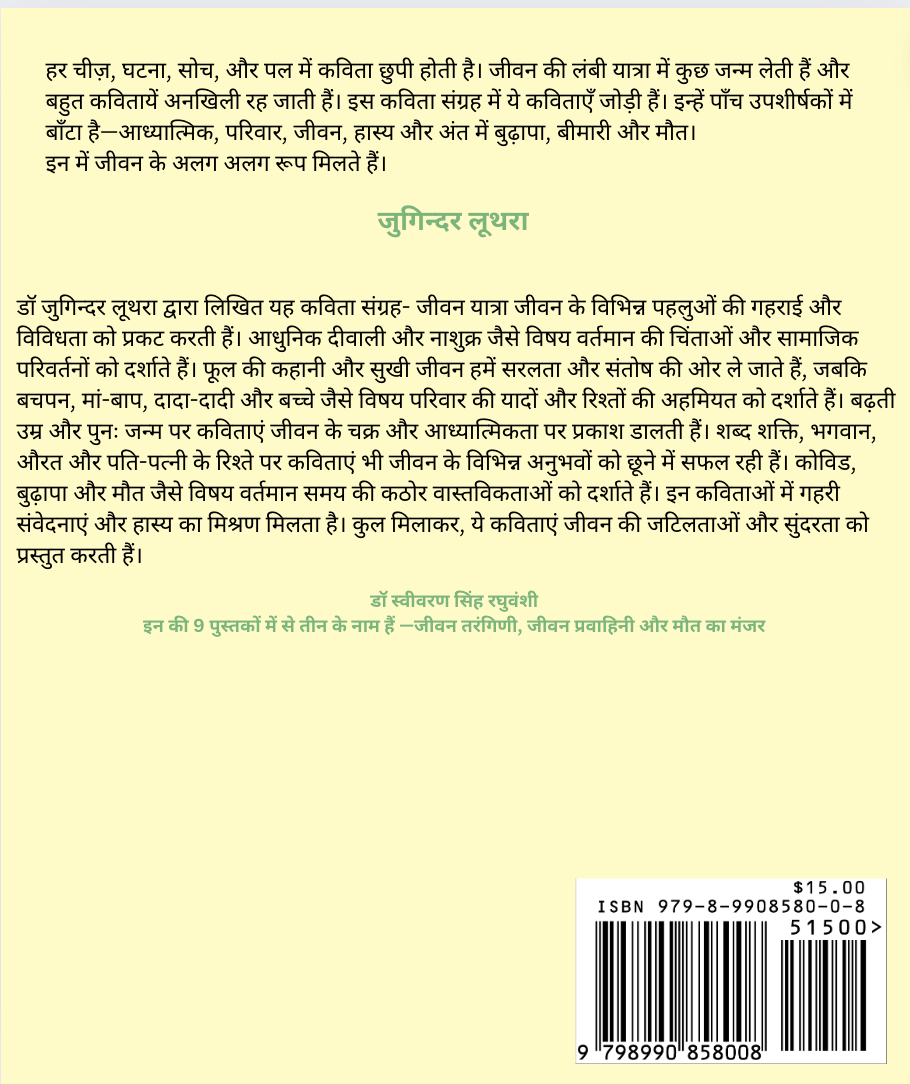
\includepdf{s24_back.png}

\end{document}
